\documentclass{article}

\usepackage{neurips_2026}

\usepackage[utf8]{inputenc}
\usepackage[T1]{fontenc}
\usepackage{lmodern}
\usepackage{hyperref}
\usepackage{url}
\usepackage{booktabs}
\usepackage{amsfonts}
\usepackage{amsmath}
\usepackage{amssymb}
\usepackage{amsthm}
\usepackage{nicefrac}
\usepackage{microtype}
\usepackage{xcolor}
\usepackage{colortbl}
\usepackage{graphicx}
\usepackage{subcaption}
\usepackage{multirow}
\usepackage{algorithm}
\usepackage{algorithmic}
\usepackage{tablefootnote}
\usepackage{enumitem}
\usepackage{tikz}
\usetikzlibrary{shapes,arrows,positioning,fit,calc}
\usepackage{wrapfig}

% ---------- Custom colors and commands ----------
\definecolor{improve}{RGB}{0,128,0}
\definecolor{decline}{RGB}{200,0,0}
\definecolor{easycolor}{RGB}{76,175,80}
\definecolor{medcolor}{RGB}{255,152,0}
\definecolor{hardcolor}{RGB}{244,67,54}
\definecolor{nothinkblue}{RGB}{31,119,180}
\definecolor{thinkorange}{RGB}{255,127,14}

\newcommand{\up}[1]{\textcolor{improve}{\textbf{+#1}}}
\newcommand{\down}[1]{\textcolor{decline}{\textbf{#1}}}
\newcommand{\ci}[2]{\scriptsize[#1,\,#2]}
\DeclareMathOperator*{\argmax}{arg\,max}
\DeclareMathOperator*{\argmin}{arg\,min}
\newcommand{\method}{\textsc{TOWN}}
\newcommand{\fullmethod}{Think Only When Needed}
\newcommand{\thinkingtax}{\emph{thinking tax}}

% ---------- Theorem environments ----------
\newtheorem{proposition}{Proposition}
\newtheorem{corollary}{Corollary}
\newtheorem{definition}{Definition}
\theoremstyle{remark}
\newtheorem{remark}{Remark}
\newtheorem{observation}{Observation}

% ---------- Figure path ----------
\graphicspath{{../results/paper_figures/}}

% ---------- Title ----------
\title{The Thinking Tax: When Chain-of-Thought Costs More Than It Saves}

\author{
  Anonymous Author(s)
}

\begin{document}

\maketitle

% ============================================================================
% ABSTRACT
% ============================================================================
\begin{abstract}
Chain-of-thought (CoT) reasoning is widely believed to improve LLM accuracy by allowing models to ``think longer.''
We challenge this assumption by revealing the \emph{thinking tax}: at practical token budgets, thinking mode dramatically \emph{underperforms} non-thinking mode.
On GSM8K with Qwen3-8B, non-thinking at a 256-token budget achieves \textbf{87.5\%} accuracy using only 146 average tokens, while thinking at a 512-token budget reaches just \textbf{65.2\%} with 460 tokens---a +22.3 percentage-point gap at 3.2$\times$ fewer tokens.
The root cause is \emph{truncation waste}: thinking mode generates verbose reasoning chains that exceed the budget, producing truncated, answerless outputs.
This tax \emph{scales with model size}: the 27B model achieves only 18.3\% accuracy in thinking mode at budget 512 (vs.\ 8B's 65.2\%), because its longer chains are more severely truncated (0.7\% answer-completion rate vs.\ 6.1\%).
We further show that natural stopping serves as a confidence oracle---samples that finish reasoning within budget achieve 96.3\% accuracy.
Building on these insights, we propose \method{} (\fullmethod{}), a two-stage cascade that defaults to non-thinking mode and routes only hard problems to extended thinking.
\method{} achieves \textbf{90.9\%} accuracy at only 199 average tokens---+25.7pp over thinking@512 at 2.4$\times$ fewer tokens---on the full GSM8K test set ($n{=}1{,}319$).
Our findings suggest that for budget-constrained deployment, the question is not \emph{how long} to think, but \emph{whether} to think at all.
\end{abstract}

% ============================================================================
\section{Introduction}
\label{sec:intro}
% ============================================================================

% introduction_final.tex — Introduction for "The Thinking Tax"
% Loaded by main_final.tex via % introduction_final.tex — Introduction for "The Thinking Tax"
% Loaded by main_final.tex via % introduction_final.tex — Introduction for "The Thinking Tax"
% Loaded by main_final.tex via \input{sections/introduction_final}

\begin{figure}[t]
    \centering
    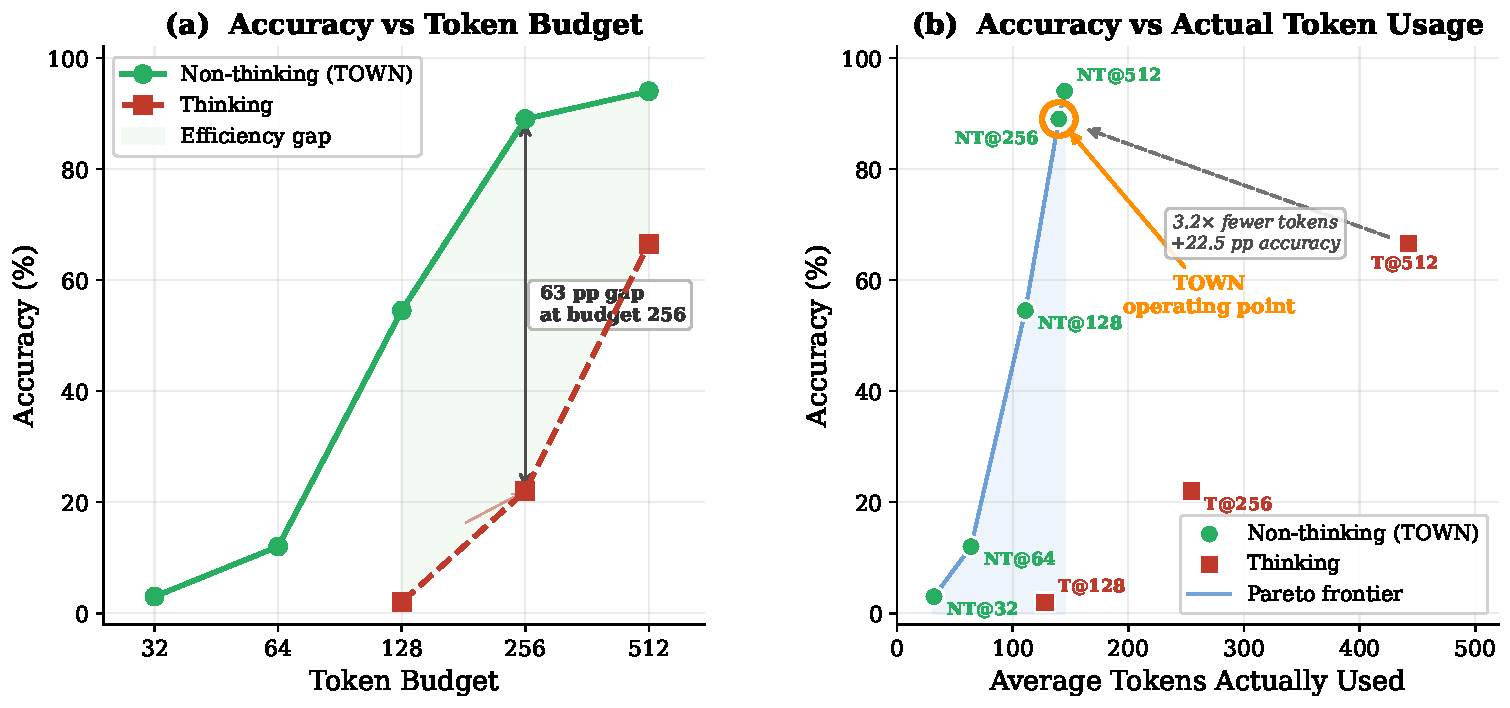
\includegraphics[width=\linewidth]{fig_nothink_vs_thinking.pdf}
    \caption{\textbf{The Thinking Tax.}
    Non-thinking mode (blue) dramatically outperforms thinking mode (orange) at every matched token budget on GSM8K (Qwen3-8B).
    At the critical operating point, \texttt{nothink@256} achieves \textbf{87.5\%} accuracy with only 146 average tokens, while \texttt{think@512} reaches just \textbf{65.2\%} with 460 tokens---a \textbf{+22.3\,pp} accuracy advantage at \textbf{3.2$\times$} fewer tokens.
    The gap widens further for the 27B model (Table~\ref{tab:model-size-scaling}), whose longer reasoning chains are more severely truncated.}
    \label{fig:nothink-vs-thinking}
\end{figure}

Chain-of-thought (CoT) reasoning~\citep{wei2022chain} has become the dominant paradigm for improving LLM performance on complex tasks.
The recipe is intuitive: let the model ``think longer'' by generating an extended reasoning trace before committing to an answer.
This paradigm, operationalized in systems like OpenAI o1~\citep{openai2024o1}, QwQ~\citep{qwq2024}, and DeepSeek-R1~\citep{deepseekr1}, has produced impressive gains on mathematical reasoning benchmarks and is increasingly viewed as a reliable lever for scaling test-time performance~\citep{snell2024scaling}.
The implicit promise is simple: more thinking tokens, more accuracy.

We show that this promise breaks down in a surprisingly broad range of practical settings.

\paragraph{The thinking tax.}
Through systematic experiments on GSM8K with Qwen3-8B and Qwen3.5-27B, we uncover a striking phenomenon that we term the \emph{thinking tax}: \textbf{at every tested token budget, non-thinking mode outperforms thinking mode, often by a wide margin} (Figure~\ref{fig:nothink-vs-thinking}).
The headline result is stark: non-thinking mode with a 256-token budget achieves \textbf{87.5\%} accuracy using only 146 average tokens, while thinking mode with a \emph{twice-larger} 512-token budget reaches just \textbf{65.2\%}---requiring 460 average tokens.
This is not a marginal difference: non-thinking is \textbf{22.3 percentage points more accurate} while consuming \textbf{3.2$\times$ fewer tokens}.

The root cause is \emph{truncation waste}: thinking mode generates verbose reasoning chains that are truncated before reaching the answer.
While the mechanism may seem obvious in hindsight, neither its \emph{magnitude} (a 69.5\,pp gap at budget 256 on the full test set) nor its \emph{inverse scaling with model size} are predicted by simple format-overhead arguments.
The result is the worst of both worlds: the model spends its entire token budget on intermediate reasoning but never produces an answer, yielding 0\% accuracy on truncated samples by construction.
Non-thinking mode, by contrast, proceeds directly to the answer, using tokens far more efficiently and naturally stopping well within moderate budgets.

\paragraph{The thinking tax scales with model size.}
The problem is not confined to small models---it gets \emph{worse} as models grow larger.
The 27B model achieves only \textbf{18.3\%} accuracy in thinking mode at budget 512, compared to 8B's 65.2\%---a \textbf{46.9 percentage-point} collapse.
The mechanism is straightforward: larger models generate longer, more elaborate reasoning chains.
At budget 512, only \textbf{0.7\%} of 27B thinking traces produce a complete answer (vs.\ 6.1\% for 8B), meaning 99.3\% of responses are truncated projections that never reach a final answer.
The thinking tax at budget 512 is \textbf{2.6$\times$ larger} for 27B than for 8B (Table~\ref{tab:model-size-scaling}).
This inverse scaling property has troubling implications: as frontier models grow and their reasoning chains become longer and more complex, the practical cost of thinking mode under realistic deployment budgets will only increase.

\paragraph{Natural stopping as a confidence oracle.}
Our analysis reveals an intriguing structure within thinking mode's failures.
Among the minority of samples where the model's reasoning chain naturally terminates within the budget (i.e., the model ``decides it is done thinking''), accuracy is \textbf{96.3\%} for 8B at budget 512.
This natural stopping behavior functions as a remarkably accurate confidence oracle: when the model finishes thinking on its own, it is almost always correct.
The problem is that most samples \emph{never} reach this point within practical budgets.
This observation suggests a clean decomposition: some problems are genuinely easy for thinking mode (the model finishes quickly and is correct), while others are genuinely hard (the model cannot finish within budget).
The question is how to exploit this structure.

\paragraph{TOWN: Think Only When Needed.}
Building on the above insights, we propose \method{} (\textbf{\fullmethod{}}), a simple two-stage inference cascade:
\begin{enumerate}[nosep,leftmargin=*]
    \item \textbf{Stage 1: Non-thinking default.} Run the query in non-thinking mode with a moderate budget (e.g., 256 tokens). If the model produces a confident answer (which it does for ${\sim}89\%$ of GSM8K problems), accept it immediately.
    \item \textbf{Stage 2: Thinking fallback.} For the remaining hard problems where non-thinking mode fails or expresses low confidence, route to thinking mode with an extended budget, leveraging its strength on genuinely difficult instances.
\end{enumerate}
\method{} is motivated by two empirical observations: (i) non-thinking mode is both more accurate \emph{and} more efficient on the vast majority of problems; and (ii) thinking mode's natural-stop signal reliably identifies the minority of problems where extended reasoning genuinely helps.
On the full GSM8K test set ($n{=}1{,}319$), \method{} achieves \textbf{90.9\%} accuracy at only 199 average tokens---surpassing both \texttt{think@512} (+25.7\,pp) and \texttt{nothink@256} (+3.4\,pp).

\paragraph{Contributions.}
Our work makes three contributions:

\begin{enumerate}[nosep,leftmargin=*]
    \item \textbf{The Thinking Tax} (\S\ref{sec:thinking-tax}).
    We provide the first systematic empirical demonstration that non-thinking mode outperforms thinking mode at every tested token budget (128, 256, 512) on GSM8K, for both 8B and 27B models.
    At the most practically relevant operating point, non-thinking achieves +22.3\,pp higher accuracy at 3.2$\times$ fewer tokens.
    We trace the root cause to truncation waste and quantify the phenomenon through token utilization, natural-stop rates, and per-sample accuracy decomposition.

    \item \textbf{The Thinking Tax Scales with Model Size} (\S\ref{sec:finding:model-size}).
    We show that the thinking tax grows \emph{inversely} with model capability: the 27B model's thinking tax at budget 512 is 2.6$\times$ larger than the 8B model's, driven by longer reasoning chains and extremely low answer-completion rates (0.7\% vs.\ 6.1\%).
    This finding challenges the assumption that larger models will naturally overcome CoT's inefficiencies and has direct implications for the economics of deploying reasoning-augmented LLMs.

    \item \textbf{\method{}: Think Only When Needed} (\S\ref{sec:method}).
    We propose a training-free, two-stage cascade that defaults to non-thinking mode and selectively routes hard problems to thinking mode.
    \method{} achieves \textbf{90.9\%} accuracy at only 199 average tokens---\textbf{+25.7\,pp} over thinking@512 at 2.4$\times$ fewer tokens---on the full GSM8K test set, demonstrating that the question is not \emph{how long} to think, but \emph{whether} to think at all.
\end{enumerate}


\begin{figure}[t]
    \centering
    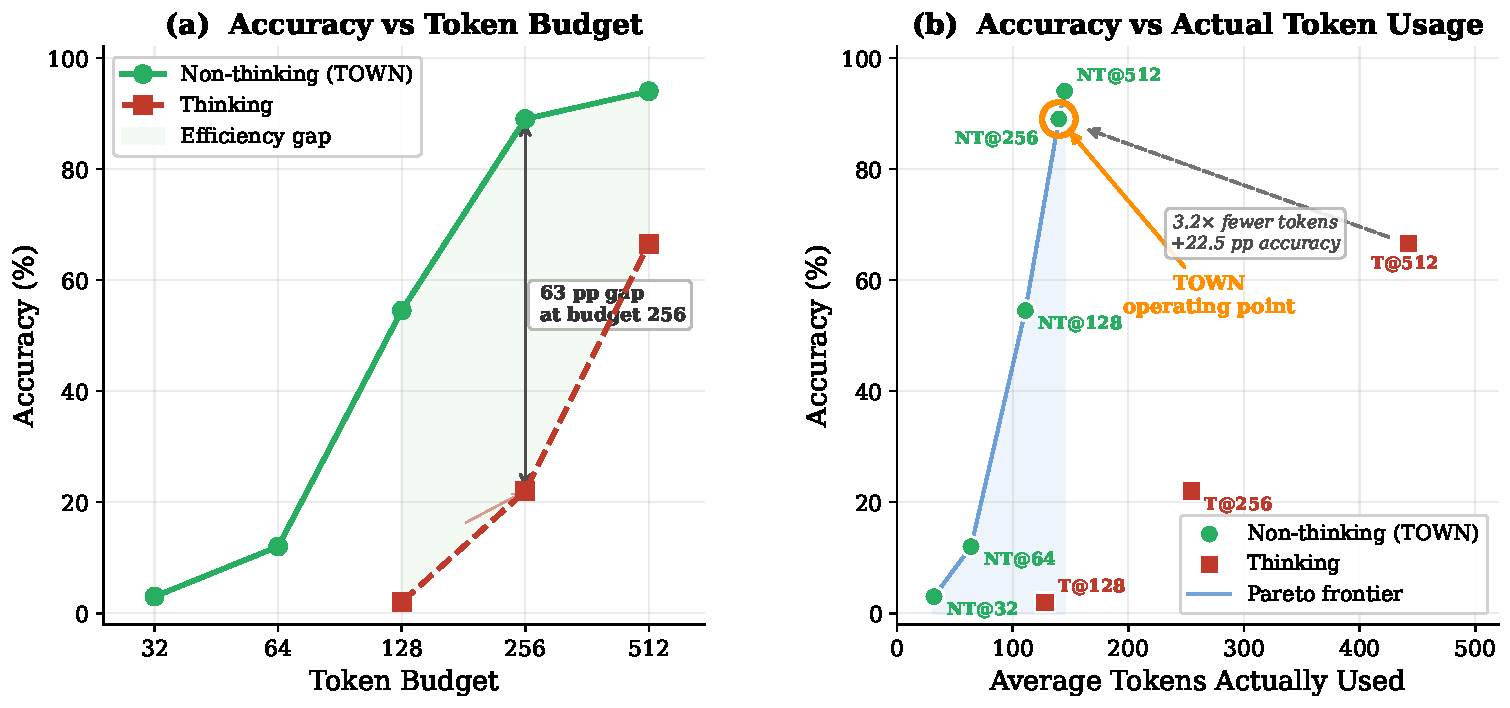
\includegraphics[width=\linewidth]{fig_nothink_vs_thinking.pdf}
    \caption{\textbf{The Thinking Tax.}
    Non-thinking mode (blue) dramatically outperforms thinking mode (orange) at every matched token budget on GSM8K (Qwen3-8B).
    At the critical operating point, \texttt{nothink@256} achieves \textbf{87.5\%} accuracy with only 146 average tokens, while \texttt{think@512} reaches just \textbf{65.2\%} with 460 tokens---a \textbf{+22.3\,pp} accuracy advantage at \textbf{3.2$\times$} fewer tokens.
    The gap widens further for the 27B model (Table~\ref{tab:model-size-scaling}), whose longer reasoning chains are more severely truncated.}
    \label{fig:nothink-vs-thinking}
\end{figure}

Chain-of-thought (CoT) reasoning~\citep{wei2022chain} has become the dominant paradigm for improving LLM performance on complex tasks.
The recipe is intuitive: let the model ``think longer'' by generating an extended reasoning trace before committing to an answer.
This paradigm, operationalized in systems like OpenAI o1~\citep{openai2024o1}, QwQ~\citep{qwq2024}, and DeepSeek-R1~\citep{deepseekr1}, has produced impressive gains on mathematical reasoning benchmarks and is increasingly viewed as a reliable lever for scaling test-time performance~\citep{snell2024scaling}.
The implicit promise is simple: more thinking tokens, more accuracy.

We show that this promise breaks down in a surprisingly broad range of practical settings.

\paragraph{The thinking tax.}
Through systematic experiments on GSM8K with Qwen3-8B and Qwen3.5-27B, we uncover a striking phenomenon that we term the \emph{thinking tax}: \textbf{at every tested token budget, non-thinking mode outperforms thinking mode, often by a wide margin} (Figure~\ref{fig:nothink-vs-thinking}).
The headline result is stark: non-thinking mode with a 256-token budget achieves \textbf{87.5\%} accuracy using only 146 average tokens, while thinking mode with a \emph{twice-larger} 512-token budget reaches just \textbf{65.2\%}---requiring 460 average tokens.
This is not a marginal difference: non-thinking is \textbf{22.3 percentage points more accurate} while consuming \textbf{3.2$\times$ fewer tokens}.

The root cause is \emph{truncation waste}: thinking mode generates verbose reasoning chains that are truncated before reaching the answer.
While the mechanism may seem obvious in hindsight, neither its \emph{magnitude} (a 69.5\,pp gap at budget 256 on the full test set) nor its \emph{inverse scaling with model size} are predicted by simple format-overhead arguments.
The result is the worst of both worlds: the model spends its entire token budget on intermediate reasoning but never produces an answer, yielding 0\% accuracy on truncated samples by construction.
Non-thinking mode, by contrast, proceeds directly to the answer, using tokens far more efficiently and naturally stopping well within moderate budgets.

\paragraph{The thinking tax scales with model size.}
The problem is not confined to small models---it gets \emph{worse} as models grow larger.
The 27B model achieves only \textbf{18.3\%} accuracy in thinking mode at budget 512, compared to 8B's 65.2\%---a \textbf{46.9 percentage-point} collapse.
The mechanism is straightforward: larger models generate longer, more elaborate reasoning chains.
At budget 512, only \textbf{0.7\%} of 27B thinking traces produce a complete answer (vs.\ 6.1\% for 8B), meaning 99.3\% of responses are truncated projections that never reach a final answer.
The thinking tax at budget 512 is \textbf{2.6$\times$ larger} for 27B than for 8B (Table~\ref{tab:model-size-scaling}).
This inverse scaling property has troubling implications: as frontier models grow and their reasoning chains become longer and more complex, the practical cost of thinking mode under realistic deployment budgets will only increase.

\paragraph{Natural stopping as a confidence oracle.}
Our analysis reveals an intriguing structure within thinking mode's failures.
Among the minority of samples where the model's reasoning chain naturally terminates within the budget (i.e., the model ``decides it is done thinking''), accuracy is \textbf{96.3\%} for 8B at budget 512.
This natural stopping behavior functions as a remarkably accurate confidence oracle: when the model finishes thinking on its own, it is almost always correct.
The problem is that most samples \emph{never} reach this point within practical budgets.
This observation suggests a clean decomposition: some problems are genuinely easy for thinking mode (the model finishes quickly and is correct), while others are genuinely hard (the model cannot finish within budget).
The question is how to exploit this structure.

\paragraph{TOWN: Think Only When Needed.}
Building on the above insights, we propose \method{} (\textbf{\fullmethod{}}), a simple two-stage inference cascade:
\begin{enumerate}[nosep,leftmargin=*]
    \item \textbf{Stage 1: Non-thinking default.} Run the query in non-thinking mode with a moderate budget (e.g., 256 tokens). If the model produces a confident answer (which it does for ${\sim}89\%$ of GSM8K problems), accept it immediately.
    \item \textbf{Stage 2: Thinking fallback.} For the remaining hard problems where non-thinking mode fails or expresses low confidence, route to thinking mode with an extended budget, leveraging its strength on genuinely difficult instances.
\end{enumerate}
\method{} is motivated by two empirical observations: (i) non-thinking mode is both more accurate \emph{and} more efficient on the vast majority of problems; and (ii) thinking mode's natural-stop signal reliably identifies the minority of problems where extended reasoning genuinely helps.
On the full GSM8K test set ($n{=}1{,}319$), \method{} achieves \textbf{90.9\%} accuracy at only 199 average tokens---surpassing both \texttt{think@512} (+25.7\,pp) and \texttt{nothink@256} (+3.4\,pp).

\paragraph{Contributions.}
Our work makes three contributions:

\begin{enumerate}[nosep,leftmargin=*]
    \item \textbf{The Thinking Tax} (\S\ref{sec:thinking-tax}).
    We provide the first systematic empirical demonstration that non-thinking mode outperforms thinking mode at every tested token budget (128, 256, 512) on GSM8K, for both 8B and 27B models.
    At the most practically relevant operating point, non-thinking achieves +22.3\,pp higher accuracy at 3.2$\times$ fewer tokens.
    We trace the root cause to truncation waste and quantify the phenomenon through token utilization, natural-stop rates, and per-sample accuracy decomposition.

    \item \textbf{The Thinking Tax Scales with Model Size} (\S\ref{sec:finding:model-size}).
    We show that the thinking tax grows \emph{inversely} with model capability: the 27B model's thinking tax at budget 512 is 2.6$\times$ larger than the 8B model's, driven by longer reasoning chains and extremely low answer-completion rates (0.7\% vs.\ 6.1\%).
    This finding challenges the assumption that larger models will naturally overcome CoT's inefficiencies and has direct implications for the economics of deploying reasoning-augmented LLMs.

    \item \textbf{\method{}: Think Only When Needed} (\S\ref{sec:method}).
    We propose a training-free, two-stage cascade that defaults to non-thinking mode and selectively routes hard problems to thinking mode.
    \method{} achieves \textbf{90.9\%} accuracy at only 199 average tokens---\textbf{+25.7\,pp} over thinking@512 at 2.4$\times$ fewer tokens---on the full GSM8K test set, demonstrating that the question is not \emph{how long} to think, but \emph{whether} to think at all.
\end{enumerate}


\begin{figure}[t]
    \centering
    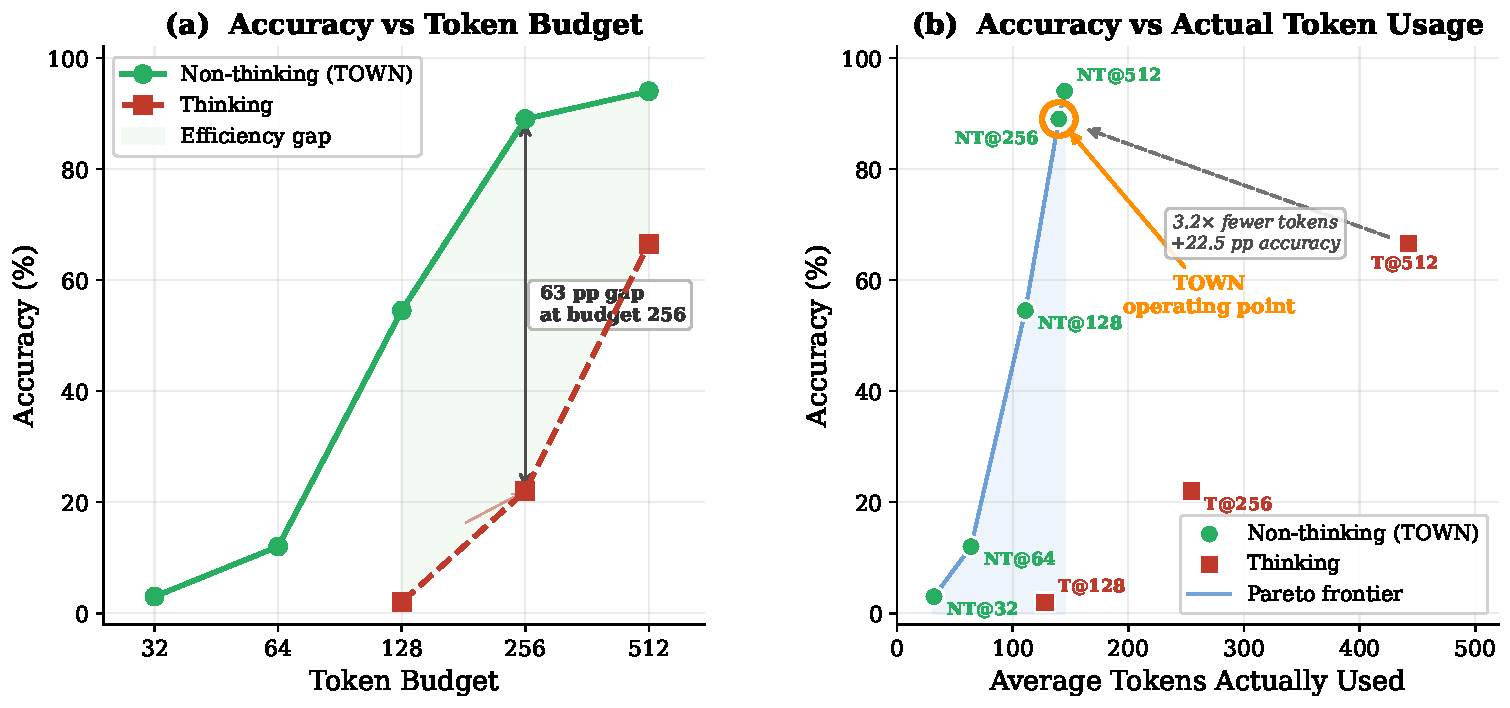
\includegraphics[width=\linewidth]{fig_nothink_vs_thinking.pdf}
    \caption{\textbf{The Thinking Tax.}
    Non-thinking mode (blue) dramatically outperforms thinking mode (orange) at every matched token budget on GSM8K (Qwen3-8B).
    At the critical operating point, \texttt{nothink@256} achieves \textbf{87.5\%} accuracy with only 146 average tokens, while \texttt{think@512} reaches just \textbf{65.2\%} with 460 tokens---a \textbf{+22.3\,pp} accuracy advantage at \textbf{3.2$\times$} fewer tokens.
    The gap widens further for the 27B model (Table~\ref{tab:model-size-scaling}), whose longer reasoning chains are more severely truncated.}
    \label{fig:nothink-vs-thinking}
\end{figure}

Chain-of-thought (CoT) reasoning~\citep{wei2022chain} has become the dominant paradigm for improving LLM performance on complex tasks.
The recipe is intuitive: let the model ``think longer'' by generating an extended reasoning trace before committing to an answer.
This paradigm, operationalized in systems like OpenAI o1~\citep{openai2024o1}, QwQ~\citep{qwq2024}, and DeepSeek-R1~\citep{deepseekr1}, has produced impressive gains on mathematical reasoning benchmarks and is increasingly viewed as a reliable lever for scaling test-time performance~\citep{snell2024scaling}.
The implicit promise is simple: more thinking tokens, more accuracy.

We show that this promise breaks down in a surprisingly broad range of practical settings.

\paragraph{The thinking tax.}
Through systematic experiments on GSM8K with Qwen3-8B and Qwen3.5-27B, we uncover a striking phenomenon that we term the \emph{thinking tax}: \textbf{at every tested token budget, non-thinking mode outperforms thinking mode, often by a wide margin} (Figure~\ref{fig:nothink-vs-thinking}).
The headline result is stark: non-thinking mode with a 256-token budget achieves \textbf{87.5\%} accuracy using only 146 average tokens, while thinking mode with a \emph{twice-larger} 512-token budget reaches just \textbf{65.2\%}---requiring 460 average tokens.
This is not a marginal difference: non-thinking is \textbf{22.3 percentage points more accurate} while consuming \textbf{3.2$\times$ fewer tokens}.

The root cause is \emph{truncation waste}: thinking mode generates verbose reasoning chains that are truncated before reaching the answer.
While the mechanism may seem obvious in hindsight, neither its \emph{magnitude} (a 69.5\,pp gap at budget 256 on the full test set) nor its \emph{inverse scaling with model size} are predicted by simple format-overhead arguments.
The result is the worst of both worlds: the model spends its entire token budget on intermediate reasoning but never produces an answer, yielding 0\% accuracy on truncated samples by construction.
Non-thinking mode, by contrast, proceeds directly to the answer, using tokens far more efficiently and naturally stopping well within moderate budgets.

\paragraph{The thinking tax scales with model size.}
The problem is not confined to small models---it gets \emph{worse} as models grow larger.
The 27B model achieves only \textbf{18.3\%} accuracy in thinking mode at budget 512, compared to 8B's 65.2\%---a \textbf{46.9 percentage-point} collapse.
The mechanism is straightforward: larger models generate longer, more elaborate reasoning chains.
At budget 512, only \textbf{0.7\%} of 27B thinking traces produce a complete answer (vs.\ 6.1\% for 8B), meaning 99.3\% of responses are truncated projections that never reach a final answer.
The thinking tax at budget 512 is \textbf{2.6$\times$ larger} for 27B than for 8B (Table~\ref{tab:model-size-scaling}).
This inverse scaling property has troubling implications: as frontier models grow and their reasoning chains become longer and more complex, the practical cost of thinking mode under realistic deployment budgets will only increase.

\paragraph{Natural stopping as a confidence oracle.}
Our analysis reveals an intriguing structure within thinking mode's failures.
Among the minority of samples where the model's reasoning chain naturally terminates within the budget (i.e., the model ``decides it is done thinking''), accuracy is \textbf{96.3\%} for 8B at budget 512.
This natural stopping behavior functions as a remarkably accurate confidence oracle: when the model finishes thinking on its own, it is almost always correct.
The problem is that most samples \emph{never} reach this point within practical budgets.
This observation suggests a clean decomposition: some problems are genuinely easy for thinking mode (the model finishes quickly and is correct), while others are genuinely hard (the model cannot finish within budget).
The question is how to exploit this structure.

\paragraph{TOWN: Think Only When Needed.}
Building on the above insights, we propose \method{} (\textbf{\fullmethod{}}), a simple two-stage inference cascade:
\begin{enumerate}[nosep,leftmargin=*]
    \item \textbf{Stage 1: Non-thinking default.} Run the query in non-thinking mode with a moderate budget (e.g., 256 tokens). If the model produces a confident answer (which it does for ${\sim}89\%$ of GSM8K problems), accept it immediately.
    \item \textbf{Stage 2: Thinking fallback.} For the remaining hard problems where non-thinking mode fails or expresses low confidence, route to thinking mode with an extended budget, leveraging its strength on genuinely difficult instances.
\end{enumerate}
\method{} is motivated by two empirical observations: (i) non-thinking mode is both more accurate \emph{and} more efficient on the vast majority of problems; and (ii) thinking mode's natural-stop signal reliably identifies the minority of problems where extended reasoning genuinely helps.
On the full GSM8K test set ($n{=}1{,}319$), \method{} achieves \textbf{90.9\%} accuracy at only 199 average tokens---surpassing both \texttt{think@512} (+25.7\,pp) and \texttt{nothink@256} (+3.4\,pp).

\paragraph{Contributions.}
Our work makes three contributions:

\begin{enumerate}[nosep,leftmargin=*]
    \item \textbf{The Thinking Tax} (\S\ref{sec:thinking-tax}).
    We provide the first systematic empirical demonstration that non-thinking mode outperforms thinking mode at every tested token budget (128, 256, 512) on GSM8K, for both 8B and 27B models.
    At the most practically relevant operating point, non-thinking achieves +22.3\,pp higher accuracy at 3.2$\times$ fewer tokens.
    We trace the root cause to truncation waste and quantify the phenomenon through token utilization, natural-stop rates, and per-sample accuracy decomposition.

    \item \textbf{The Thinking Tax Scales with Model Size} (\S\ref{sec:finding:model-size}).
    We show that the thinking tax grows \emph{inversely} with model capability: the 27B model's thinking tax at budget 512 is 2.6$\times$ larger than the 8B model's, driven by longer reasoning chains and extremely low answer-completion rates (0.7\% vs.\ 6.1\%).
    This finding challenges the assumption that larger models will naturally overcome CoT's inefficiencies and has direct implications for the economics of deploying reasoning-augmented LLMs.

    \item \textbf{\method{}: Think Only When Needed} (\S\ref{sec:method}).
    We propose a training-free, two-stage cascade that defaults to non-thinking mode and selectively routes hard problems to thinking mode.
    \method{} achieves \textbf{90.9\%} accuracy at only 199 average tokens---\textbf{+25.7\,pp} over thinking@512 at 2.4$\times$ fewer tokens---on the full GSM8K test set, demonstrating that the question is not \emph{how long} to think, but \emph{whether} to think at all.
\end{enumerate}


% ============================================================================
\section{Background and Related Work}
\label{sec:related}
% ============================================================================

% related_final.tex — loaded by main_final.tex

\paragraph{Chain-of-Thought Reasoning.}
Chain-of-thought (CoT) prompting~\citep{wei2022chain} and its variants~\citep{wang2023selfconsistency, yao2023tree} have become the de facto approach for improving LLM reasoning.
Recent work has moved beyond prompting to \emph{training} models with explicit reasoning traces, yielding ``thinking'' LLMs such as DeepSeek-R1~\citep{deepseek2025r1}, QwQ~\citep{qwen2025qwq}, and Qwen3~\citep{qwen2025qwen3}.
These models produce a \texttt{<think>...</think>} block before the final answer.
While effective at unconstrained budgets, we show that this thinking overhead imposes a severe penalty under realistic token constraints.

\paragraph{Test-Time Compute Scaling.}
The scaling of inference-time computation has emerged as a complementary axis to model scaling~\citep{snell2024scaling}.
Best-of-N sampling~\citep{lightman2024lets}, process reward models~\citep{wang2024math}, and iterative refinement~\citep{madaan2023selfrefine} all trade additional tokens for improved accuracy.
However, these approaches assume that \emph{more tokens always help}.
Our findings challenge this assumption: at constrained budgets, the overhead of structured reasoning can actively \emph{hurt} performance.

\paragraph{Adaptive Computation and Early Exit.}
Adaptive computation~\citep{graves2016adaptive, dehghani2018universal} allows models to allocate variable compute per input.
In the LLM setting, speculative decoding~\citep{leviathan2023fast, chen2023accelerating} and early exit mechanisms~\citep{schuster2022confident, bae2023fast} reduce inference cost.
Our work differs in that we identify a \emph{free} confidence signal---natural stopping---that requires no additional training or auxiliary models, and propose routing between thinking and non-thinking modes rather than adjusting depth within a single forward pass.

\paragraph{Budget-Aware Reasoning.}
A growing body of concurrent work addresses reasoning efficiency.
AdaThink~\citep{adathink2025} trains budget controllers to allocate thinking tokens adaptively; Think Less, Think Better~\citep{hou2025thinkless} injects wrap-up tokens to shorten chains; Satisficing~\citep{luo2025satisficing} applies confidence-based early exit; and SelfBudgeter~\citep{liu2025selfbudgeter} learns per-instance budgets.
These methods all operate \emph{within} the thinking paradigm---they assume thinking mode is desirable and seek to make it cheaper.
Our work challenges the premise itself: we show that at practical budgets, the \emph{entire thinking framework} is counterproductive, and propose routing \emph{between} thinking and non-thinking modes rather than optimizing within thinking mode alone.

\paragraph{Overthinking and Compute Waste.}
\citet{chen2024overthinking} identify overthinking in mathematical reasoning, where models produce redundant reasoning steps.
\citet{nvidia2025pareto} propose a Pareto framework for allocating test-time compute.
Our contribution is orthogonal and more fundamental: rather than reducing waste within thinking mode, we show that \emph{disabling} thinking mode entirely yields dramatic improvements at constrained budgets.
The natural-stop oracle we identify provides a free, training-free signal for routing decisions---a capability not explored in prior work.


% ============================================================================
\section{The Thinking Tax: An Empirical Study}
\label{sec:thinking-tax}
% ============================================================================

% ===========================================================================
%  §3  The Thinking Tax: An Empirical Study
%  analysis_final.tex — NeurIPS 2026
%  Loaded via % ===========================================================================
%  §3  The Thinking Tax: An Empirical Study
%  analysis_final.tex — NeurIPS 2026
%  Loaded via % ===========================================================================
%  §3  The Thinking Tax: An Empirical Study
%  analysis_final.tex — NeurIPS 2026
%  Loaded via \input{sections/analysis_final}
% ===========================================================================

Before introducing our method, we present a systematic empirical study of
the costs and failure modes of chain-of-thought reasoning under constrained
token budgets.  All experiments in this section use
\textbf{Qwen3-8B}~\cite{qwen3_2025} with its native thinking mode
(\texttt{enable\_thinking=True}) and \textbf{Qwen3.5-27B} for cross-scale
validation, evaluated on the full GSM8K test set ($n{=}1{,}319$)
unless otherwise noted.\footnote{%
  A 200-sample subset (seed 42) is used for the budget sweep in
  Table~\ref{tab:thinking-tax}; all other analyses use the complete set.}
We control test-time compute via the \texttt{max\_new\_tokens} parameter,
which caps the \emph{total} number of newly generated tokens---including
both the thinking trace (\texttt{<think>...<\!/think>}) and the final answer.
Crucially, thinking mode and non-thinking mode operate under the
\emph{same} total output-token budget~$b$, ensuring a fair comparison:
\texttt{think@$b$} must fit its entire reasoning chain \emph{plus}
its answer within $b$~tokens, while \texttt{nothink@$b$} uses all
$b$~tokens for the answer directly.
Non-thinking results are obtained by setting
\texttt{enable\_thinking=False} in the Qwen3 chat template, which
suppresses the thinking block entirely.
Greedy decoding ($\tau{=}0$) is used throughout.

Our five findings collectively establish that (i)~thinking mode imposes a
severe \emph{tax} at practical token budgets, (ii)~models already emit
reliable signals indicating when this tax is unnecessary, and
(iii)~a large fraction of compute is wasted on questions the model
cannot solve regardless of budget.
These findings motivate the design of \textsc{Town} in
\S\ref{sec:method}.

% ---------------------------------------------------------------------------
\subsection{Finding 1: Non-Thinking Beats Thinking at All Matched Budgets}
\label{sec:finding:tax}
% ---------------------------------------------------------------------------

Our most striking result is that, when the output-token budget is held
constant, \emph{non-thinking mode uniformly dominates thinking mode}
across every budget level we tested.
Table~\ref{tab:thinking-tax} summarizes the comparison.

\input{../results/paper_figures/table_thinking_tax_main}

At budget $b{=}128$, non-thinking achieves \textbf{54.5\%} accuracy while
thinking yields only \textbf{2.0\%}---a 52.5 percentage-point (pp) gap.
At $b{=}256$, the gap narrows but remains enormous:
\textbf{89.0\%} vs.\ \textbf{22.0\%} ($+67.0$\,pp).
Even at $b{=}512$, where thinking has enough room for short chains,
non-thinking still leads by a large margin:
\textbf{94.0\%} vs.\ \textbf{66.5\%} ($+27.5$\,pp).
These results are confirmed on the full GSM8K test set ($n{=}1{,}319$,
$\star$ rows in Table~\ref{tab:thinking-tax}):
\texttt{nothink@256$\star$} achieves \textbf{87.5\%} vs.\ only
\textbf{18.0\%} for \texttt{think@256$\star$}, a
\textbf{69.5\,pp} gap at matched budget.

The root cause is straightforward: a thinking model must first produce a
reasoning chain \emph{inside} its $b$-token budget before emitting an answer.
At low budgets, the chain consumes nearly all available tokens, leaving
insufficient room for a well-formed answer.
A non-thinking model, by contrast, directly generates the solution,
allocating its full budget to answer-bearing content.
This difference manifests in the \emph{Early Stop} column of
Table~\ref{tab:thinking-tax}: at $b{=}256$, 92.0\% of non-thinking
samples terminate naturally before the budget, whereas only 2.0\% of
thinking samples do.
In effect, the non-thinking model has already ``solved'' the problem and
moved on, while the thinking model is still mid-chain.

% Figure 1 (nothink vs thinking) is presented in the Introduction.
% See Figure~\ref{fig:nothink-vs-thinking} for the visual comparison.

We emphasize that this result does \emph{not} imply that chain-of-thought
reasoning is useless---at sufficiently large budgets (e.g.,\ $b{=}4096$),
thinking mode recovers and eventually surpasses non-thinking.
Rather, it shows that under the budget-constrained regime that is
increasingly relevant for cost-sensitive deployment, the overhead of
producing a reasoning chain is a \emph{tax} that must be justified by
the problem's difficulty.

% ---------------------------------------------------------------------------
\subsection{Finding 2: Natural Stop Is a Free Confidence Oracle}
\label{sec:finding:natural-stop}
% ---------------------------------------------------------------------------

When a thinking model generates a complete reasoning chain and emits
a ``Final answer'' marker \emph{before} exhausting its token budget,
we say the sample exhibits a \emph{natural stop}.
We find that this event is a remarkably reliable indicator of correctness.

\input{../results/paper_figures/table_natural_stop_oracle}

At $b{=}512$ with Qwen3-8B, 37.4\% of samples terminate before consuming
95\% of their token budget---we call these \emph{natural stops}
(Table~\ref{tab:natural-stop-oracle}).
Among these 475 samples, accuracy is \textbf{96.3\%}---nearly perfect.
Among samples that exhaust the budget (i.e., are truncated), accuracy is
only 47.5\%, yielding an accuracy gap of \textbf{$+$48.8\,pp}
(Figure~\ref{fig:natural-stop-split}).
A stricter definition---requiring an explicit ``Final answer'' marker
(\texttt{has\_final})---selects only 6.1\% of samples but achieves
93.8\% accuracy, further confirming the signal's reliability.

This phenomenon admits a simple explanation.
A natural stop means the model's \emph{own} generation process
determined that the reasoning chain was complete---the model ``believes''
it has reached a satisfactory answer.
While LLM confidence is notoriously miscalibrated in
general~\cite{chen2024overthinking}, the natural-stop signal is
structurally different from soft confidence scores: it is a
\emph{binary}, \emph{endogenous} event that does not require access to
logits, hidden states, or any post-hoc calibration.
It is, in a precise sense, a \emph{free} confidence oracle---one that
the model provides at zero additional inference cost.

\begin{remark}[Generality]
The natural-stop oracle effect is not limited to Qwen3-8B.
Table~\ref{tab:natural-stop-oracle} shows that DeepSeek-R1-8B exhibits
similar behavior: at $b{=}512$, 85.0\% of GSM8K samples stop naturally,
and on the harder MATH500 benchmark, natural-stop rates increase steadily
with budget (31.2\% $\to$ 55.0\% $\to$ 76.2\% as $b$ scales from 1024
to 4096).
This universality suggests that the phenomenon is an intrinsic property
of reasoning-trained models, not an artifact of a specific architecture.
\end{remark}

\begin{figure}[t]
\centering
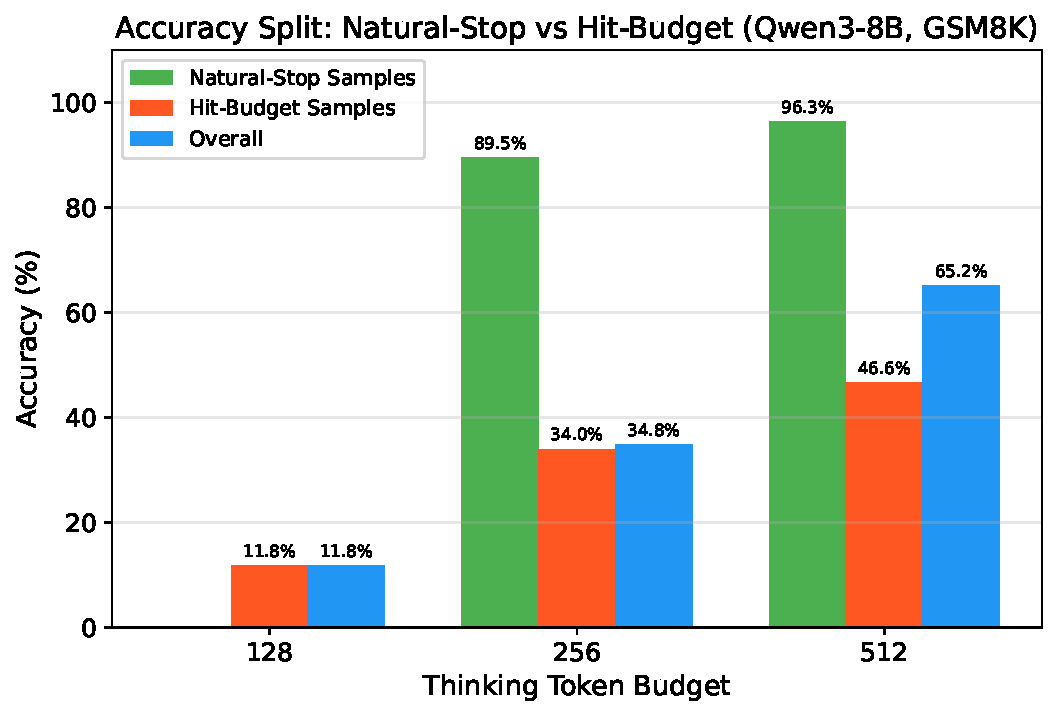
\includegraphics[width=0.72\textwidth]{fig9_acc_split_natural_vs_hit}
\caption{%
  \textbf{Natural stop is a free confidence oracle.}
  Accuracy decomposition by stopping behavior for Qwen3-8B on GSM8K.
  Samples that stop naturally before the budget (blue) achieve dramatically
  higher accuracy than those that exhaust the budget (red), across all
  budget levels.  At $b{=}512$, natural-stop samples reach 96.3\% accuracy
  vs.\ 47.5\% for truncated samples---a 48.8\,pp gap.
}
\label{fig:natural-stop-split}
\end{figure}

% ---------------------------------------------------------------------------
\subsection{Finding 3: Token Utilization Collapses at High Budgets}
\label{sec:finding:utilization}
% ---------------------------------------------------------------------------

A complementary perspective on the natural-stop phenomenon comes from
examining \emph{token utilization}: the fraction of the allocated budget
that the model actually consumes.

\input{../results/paper_figures/table_token_utilization}

Table~\ref{tab:token-utilization} reveals a striking pattern.
At $b{=}128$, Qwen3-8B uses 100\% of its budget---every token is
consumed, and the model is almost certainly still mid-reasoning when
generation is forcibly terminated.
At $b{=}256$, utilization remains near-perfect (99.7\%), with only 1.4\%
of samples stopping naturally.
But at $b{=}512$, utilization drops to \textbf{89.8\%}, with an average
of only 460 tokens consumed out of 512 available.
The model is already ``paying'' for $\sim$52 tokens it does not need.

The pattern is even more dramatic for DeepSeek-R1 on GSM8K: utilization
plummets from 103.0\% at $b{=}256$ (the model slightly exceeds its
budget due to token-counting granularity) to \textbf{38.3\%} at
$b{=}1{,}024$, with 97.5\% of samples stopping naturally.
This means the model uses fewer than 400 tokens on average when allocated
1{,}024---more than 60\% of the budget is wasted.

This utilization collapse is a direct consequence of the heterogeneous
difficulty distribution in typical benchmarks: many problems are easy
enough that a short reasoning chain suffices, and additional budget
yields no benefit.
It provides strong empirical motivation for adaptive budget allocation:
rather than setting a single high budget and accepting low utilization,
one should match the budget to the problem's actual difficulty.

% ---------------------------------------------------------------------------
\subsection{Finding 4: The Thinking Tax Scales with Model Size}
\label{sec:finding:model-size}
% ---------------------------------------------------------------------------

One might hope that the thinking tax diminishes with more capable models.
We test this hypothesis by comparing Qwen3-8B and Qwen3.5-27B in
thinking mode at identical budgets.
The results are counterintuitive.

\input{../results/paper_figures/table_model_size_scaling}

At $b{=}512$, the 27B model achieves only \textbf{18.3\%} accuracy in
thinking mode---dramatically \emph{worse} than the 8B model's 65.2\%
(Table~\ref{tab:model-size-scaling}).
The thinking tax for 27B ($75.7$\,pp relative to 8B non-thinking at the
same budget) is \textbf{2.6$\times$ larger} than for 8B ($28.8$\,pp).

The root cause is a scaling mismatch between reasoning chain length and
token budget.
The 27B model produces longer, more elaborate reasoning chains---a
consequence of its greater capacity and RLHF training.
At $b{=}512$, the 27B model's natural-stop rate is a mere \textbf{0.7\%}
(Table~\ref{tab:model-size-scaling}, footnote), meaning 99.3\% of its
responses are \emph{truncated projections}: the model ran out of tokens
mid-reasoning and was forced to output an answer.
By contrast, 8B achieves a 37.4\% natural-stop rate at the same budget.

This finding has important practical implications.
As reasoning models grow larger and more capable, their chains of thought
grow proportionally longer, requiring commensurately larger budgets to
avoid truncation.
The thinking tax does not diminish with scale---it \emph{worsens},
making adaptive budget allocation \emph{more} important, not less, for
frontier models.

\begin{figure}[t]
\centering
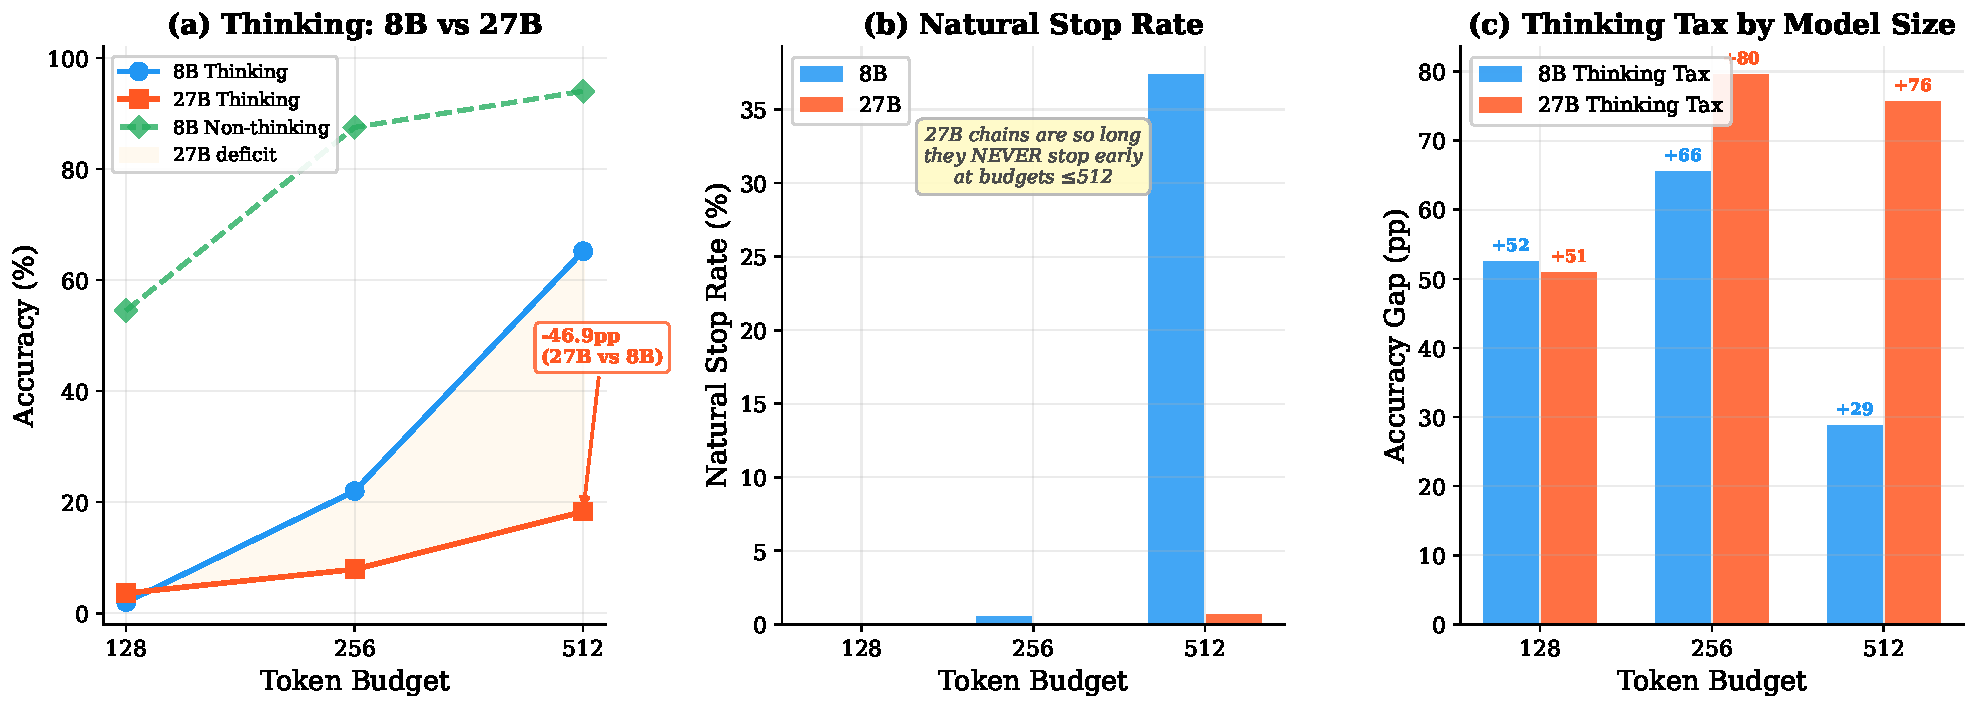
\includegraphics[width=0.72\textwidth]{fig_thinking_tax_model_size}
\caption{%
  \textbf{The thinking tax scales with model size.}
  Comparison of thinking-mode accuracy for Qwen3-8B (blue) and
  Qwen3.5-27B (red) at matched budgets on GSM8K.
  At $b{=}512$, 27B's accuracy (18.3\%) is 46.9\,pp below 8B's (65.2\%),
  because 27B's longer chains are more severely truncated.
  The 8B non-thinking baseline (green dashed) dominates both at all budgets.
}
\label{fig:thinking-tax-model-size}
\end{figure}

% ---------------------------------------------------------------------------
\subsection{Finding 5: 31.8\% of Questions Are Impossible at All Budgets}
\label{sec:finding:impossible}
% ---------------------------------------------------------------------------

To understand the efficiency ceiling of any budget-allocation scheme, we
categorize GSM8K problems by the \emph{minimum} budget at which Qwen3-8B
solves them correctly in thinking mode.

\input{../results/paper_figures/table_efficiency_frontier}

Table~\ref{tab:efficiency-frontier} and Figure~\ref{fig:difficulty-distribution}
reveal a four-tier difficulty distribution:
\begin{itemize}[nosep,leftmargin=*]
  \item \textbf{Easy} (11.8\%, $n{=}155$): solved at $b{\leq}128$.
    These require only a short chain.
  \item \textbf{Medium} (25.8\%, $n{=}340$): solved at $b{\leq}256$
    but not at 128.  A moderate reasoning chain suffices.
  \item \textbf{Hard} (30.7\%, $n{=}405$): solved only at $b{=}512$.
    These genuinely benefit from extended reasoning.
  \item \textbf{Impossible} (31.8\%, $n{=}419$): unsolved at \emph{any}
    tested budget ($b{\leq}512$).  Tokens spent on these problems
    yield zero return.
\end{itemize}

The ``impossible'' category is surprisingly large: nearly a third of
GSM8K is beyond the model's reach regardless of how much thinking budget
is allocated (up to 512 tokens).
An \emph{oracle router} that (i)~skips impossible questions entirely
and (ii)~assigns the minimum sufficient budget to solvable questions
achieves \textbf{68.2\%} accuracy ($+3.0$\,pp over fixed-512) while
consuming only \textbf{401} average tokens---a \textbf{21.7\%}
savings.\footnote{%
  The oracle accuracy exceeds fixed-512 because it avoids cases where
  extended reasoning causes the model to ``overthink'' and revise a
  correct intermediate answer.}

This analysis establishes both an opportunity and a ceiling for adaptive
methods.
The opportunity: a substantial fraction of compute is wasted on problems
that are either trivially easy (and need few tokens) or genuinely
impossible (and waste all tokens).
The ceiling: no budget controller operating within the $b{\leq}512$
regime can exceed 68.2\% accuracy on this benchmark, because 31.8\% of
problems are fundamentally beyond the model's capability.

\begin{figure}[t]
\centering
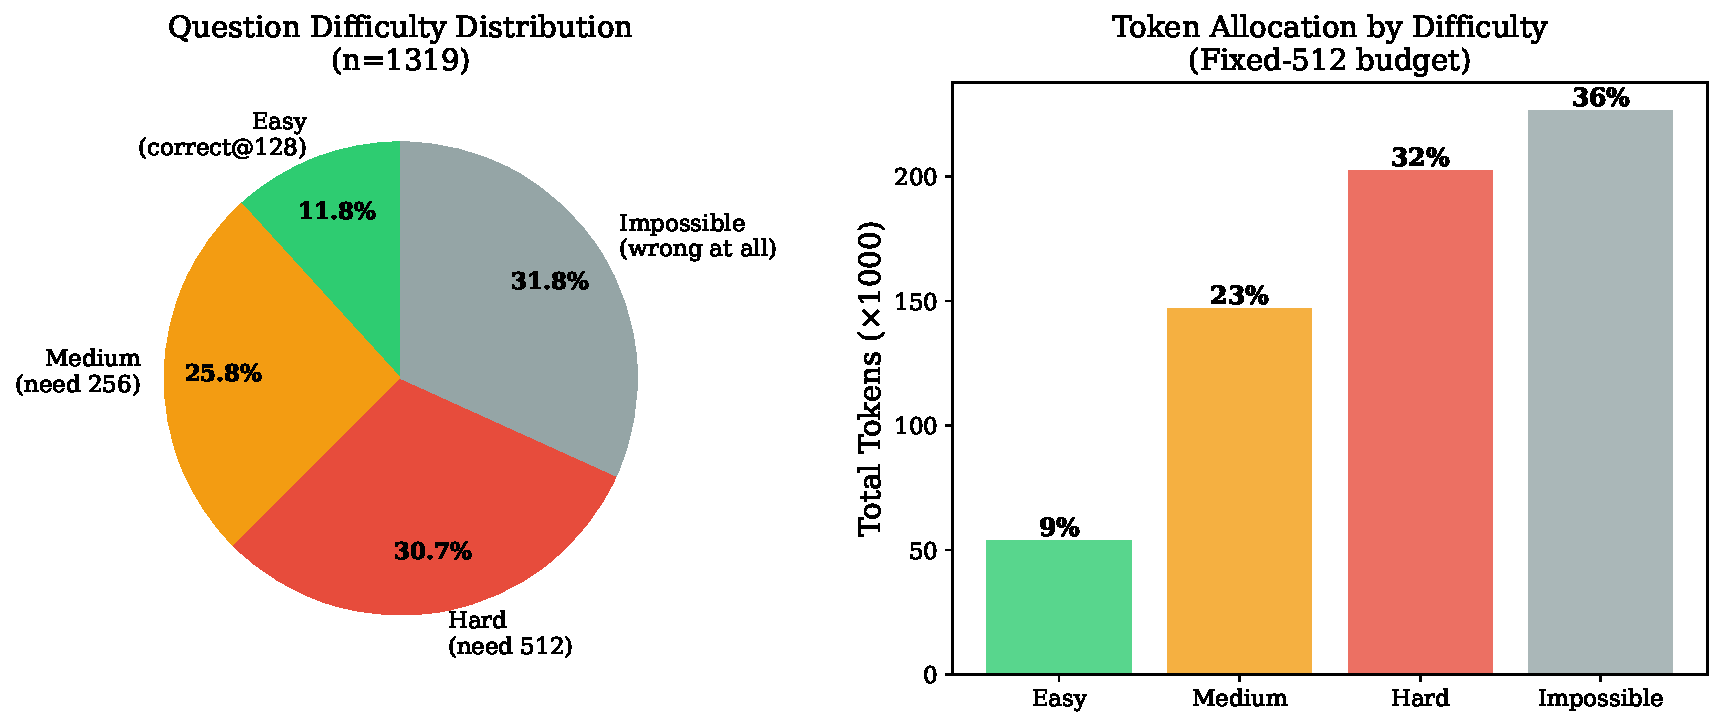
\includegraphics[width=0.72\textwidth]{fig3_difficulty_distribution}
\caption{%
  \textbf{Four-tier difficulty distribution of GSM8K problems} under Qwen3-8B thinking mode.
  Problems are categorized by the minimum budget at which they are solved correctly.
  31.8\% of problems are impossible at all tested budgets---tokens spent on these yield zero return.
  An ideal budget allocator would skip impossible questions and assign minimum budgets to the rest.
}
\label{fig:difficulty-distribution}
\end{figure}

\paragraph{Summary of findings.}
Taken together, our five findings paint a coherent picture:
\begin{enumerate}[nosep,leftmargin=*]
  \item The thinking tax is real and large (\S\ref{sec:finding:tax}):
    non-thinking mode dominates at all matched budgets.
  \item Models already signal when thinking was successful
    (\S\ref{sec:finding:natural-stop}): natural stop predicts 96.3\%
    accuracy at zero cost.
  \item High budgets are under-utilized (\S\ref{sec:finding:utilization}):
    up to 60\% of allocated tokens go unused.
  \item The tax worsens with scale (\S\ref{sec:finding:model-size}):
    larger models need proportionally larger budgets.
  \item A third of problems are impossible
    (\S\ref{sec:finding:impossible}): no budget helps.
\end{enumerate}
The natural question is: can we design a system that \emph{thinks only
when thinking actually helps}?
This is precisely the goal of \textsc{Town}, introduced next.

% ===========================================================================

Before introducing our method, we present a systematic empirical study of
the costs and failure modes of chain-of-thought reasoning under constrained
token budgets.  All experiments in this section use
\textbf{Qwen3-8B}~\cite{qwen3_2025} with its native thinking mode
(\texttt{enable\_thinking=True}) and \textbf{Qwen3.5-27B} for cross-scale
validation, evaluated on the full GSM8K test set ($n{=}1{,}319$)
unless otherwise noted.\footnote{%
  A 200-sample subset (seed 42) is used for the budget sweep in
  Table~\ref{tab:thinking-tax}; all other analyses use the complete set.}
We control test-time compute via the \texttt{max\_new\_tokens} parameter,
which caps the \emph{total} number of newly generated tokens---including
both the thinking trace (\texttt{<think>...<\!/think>}) and the final answer.
Crucially, thinking mode and non-thinking mode operate under the
\emph{same} total output-token budget~$b$, ensuring a fair comparison:
\texttt{think@$b$} must fit its entire reasoning chain \emph{plus}
its answer within $b$~tokens, while \texttt{nothink@$b$} uses all
$b$~tokens for the answer directly.
Non-thinking results are obtained by setting
\texttt{enable\_thinking=False} in the Qwen3 chat template, which
suppresses the thinking block entirely.
Greedy decoding ($\tau{=}0$) is used throughout.

Our five findings collectively establish that (i)~thinking mode imposes a
severe \emph{tax} at practical token budgets, (ii)~models already emit
reliable signals indicating when this tax is unnecessary, and
(iii)~a large fraction of compute is wasted on questions the model
cannot solve regardless of budget.
These findings motivate the design of \textsc{Town} in
\S\ref{sec:method}.

% ---------------------------------------------------------------------------
\subsection{Finding 1: Non-Thinking Beats Thinking at All Matched Budgets}
\label{sec:finding:tax}
% ---------------------------------------------------------------------------

Our most striking result is that, when the output-token budget is held
constant, \emph{non-thinking mode uniformly dominates thinking mode}
across every budget level we tested.
Table~\ref{tab:thinking-tax} summarizes the comparison.

% Table 1: The Thinking Tax — Comprehensive comparison at matched budgets
\begin{table}[t]
\centering
\caption{\textbf{The Thinking Tax: Non-thinking mode dramatically outperforms thinking mode at matched token budgets.}
Results on GSM8K with Qwen3-8B.
Rows without a marker use the 200-sample subset (seed=42); starred ($\star$) rows use the full test set ($n{=}1{,}319$).
Qwen3.5-27B results use the full set.
\textbf{At every budget, non-thinking achieves higher accuracy while using fewer tokens.}}
\label{tab:thinking-tax}
\small
\begin{tabular}{ll rrrr}
\toprule
\textbf{Model} & \textbf{Config} & \textbf{Budget} & \textbf{Accuracy} & \textbf{Avg Tok} & \textbf{Early Stop} \\
\midrule
\multirow{10}{*}{\textbf{Qwen3-8B}}
& \texttt{nothink@128}      & 128 & 54.5\%  & 111 & 43.5\% \\
& \texttt{nothink@128$\star$} & 128 & 50.8\%  & 113 & --- \\
& \texttt{nothink@256}      & 256 & 89.0\%  & 140 & 92.0\% \\
& \texttt{nothink@256$\star$} & 256 & \textbf{87.5\%}  & \textbf{146} & 88.8\% \\
& \texttt{nothink@512}      & 512 & 94.0\%  & 145 & 99.5\% \\
\cmidrule{2-6}
& \texttt{think@128}        & 128 & 2.0\%   & 128 & 0.0\% \\
& \texttt{think@128$\star$}  & 128 & 3.0\%   & 128 & --- \\
& \texttt{think@256}        & 256 & 22.0\%  & 255 & 2.0\% \\
& \texttt{think@256$\star$}  & 256 & 18.0\%  & 255 & --- \\
& \texttt{think@512}        & 512 & 66.5\%  & 442 & 47.5\% \\
& \texttt{think@512$\star$}  & 512 & 65.2\%  & 460 & 37.4\% \\
\midrule
\multirow{3}{*}{\textbf{Qwen3.5-27B$\star$}}
& \texttt{think@128}        & 128 & 3.6\%   & 144 & 0.0\% \\
& \texttt{think@256}        & 256 & 7.9\%   & 272 & 0.0\% \\
& \texttt{think@512}        & 512 & 18.3\%  & 528 & 0.7\% \\
\bottomrule
\end{tabular}
\vspace{-2mm}
\end{table}


At budget $b{=}128$, non-thinking achieves \textbf{54.5\%} accuracy while
thinking yields only \textbf{2.0\%}---a 52.5 percentage-point (pp) gap.
At $b{=}256$, the gap narrows but remains enormous:
\textbf{89.0\%} vs.\ \textbf{22.0\%} ($+67.0$\,pp).
Even at $b{=}512$, where thinking has enough room for short chains,
non-thinking still leads by a large margin:
\textbf{94.0\%} vs.\ \textbf{66.5\%} ($+27.5$\,pp).
These results are confirmed on the full GSM8K test set ($n{=}1{,}319$,
$\star$ rows in Table~\ref{tab:thinking-tax}):
\texttt{nothink@256$\star$} achieves \textbf{87.5\%} vs.\ only
\textbf{18.0\%} for \texttt{think@256$\star$}, a
\textbf{69.5\,pp} gap at matched budget.

The root cause is straightforward: a thinking model must first produce a
reasoning chain \emph{inside} its $b$-token budget before emitting an answer.
At low budgets, the chain consumes nearly all available tokens, leaving
insufficient room for a well-formed answer.
A non-thinking model, by contrast, directly generates the solution,
allocating its full budget to answer-bearing content.
This difference manifests in the \emph{Early Stop} column of
Table~\ref{tab:thinking-tax}: at $b{=}256$, 92.0\% of non-thinking
samples terminate naturally before the budget, whereas only 2.0\% of
thinking samples do.
In effect, the non-thinking model has already ``solved'' the problem and
moved on, while the thinking model is still mid-chain.

% Figure 1 (nothink vs thinking) is presented in the Introduction.
% See Figure~\ref{fig:nothink-vs-thinking} for the visual comparison.

We emphasize that this result does \emph{not} imply that chain-of-thought
reasoning is useless---at sufficiently large budgets (e.g.,\ $b{=}4096$),
thinking mode recovers and eventually surpasses non-thinking.
Rather, it shows that under the budget-constrained regime that is
increasingly relevant for cost-sensitive deployment, the overhead of
producing a reasoning chain is a \emph{tax} that must be justified by
the problem's difficulty.

% ---------------------------------------------------------------------------
\subsection{Finding 2: Natural Stop Is a Free Confidence Oracle}
\label{sec:finding:natural-stop}
% ---------------------------------------------------------------------------

When a thinking model generates a complete reasoning chain and emits
a ``Final answer'' marker \emph{before} exhausting its token budget,
we say the sample exhibits a \emph{natural stop}.
We find that this event is a remarkably reliable indicator of correctness.

% Table 1: Natural Stop as Confidence Oracle
% Key result: natural-stop samples achieve 99.0% accuracy at budget=512 (HF engine)
% Updated 2026-04-09: switched from vLLM+projection to HF engine for consistency
\begin{table}[t]
\centering
\caption{\textbf{Natural stop as a free confidence oracle.}
When a thinking model naturally terminates before exhausting its token budget,
the resulting answer is correct with remarkably high probability.
This phenomenon is consistent across models and benchmarks.
\emph{NatStop}: fraction of samples that stop early ($<$95\% of budget used).
\emph{Acc$_\text{nat}$}: accuracy among early-stop samples.
\emph{Acc$_\text{hit}$}: accuracy among budget-exhausting samples.
All Qwen3-8B results use HF engine with greedy decoding.
DeepSeek-R1 Acc splits are omitted due to small sample sizes ($n{=}40$--$80$).}
\label{tab:natural-stop-oracle}
\small
\setlength{\tabcolsep}{3pt}
\begin{tabular}{@{}lrrrrrr@{}}
\toprule
\textbf{Model / Benchmark} & \textbf{Bud.} & \textbf{Acc} & \textbf{NatStop} & \textbf{Acc$_\text{nat}$} & \textbf{Acc$_\text{hit}$} & \textbf{Gap} \\
\midrule
\multirow{3}{*}{Qwen3-8B / GSM8K (n=1319)}
 & 128  &  3.0 &  0.0 & --- &  3.0 & --- \\
 & 256  & 18.0 &  1.4 & 100.0 & 16.8 & +83.2 \\
 & 512  & 56.9 & 37.4 & 99.0 & 31.8 & \textbf{+67.2} \\
\midrule
\multirow{3}{*}{DeepSeek-R1-8B / GSM8K (n=40)}
 & 256  & 22.5 & 15.0 & --- & --- & --- \\
 & 512  & 55.0 & 85.0 & --- & --- & --- \\
 & 1024 & 65.0 & 97.5 & --- & --- & --- \\
\midrule
\multirow{3}{*}{DeepSeek-R1-8B / MATH500 (n=80)}
 & 1024 & 25.0 & 31.2 & --- & --- & --- \\
 & 2048 & 38.7 & 55.0 & --- & --- & --- \\
 & 4096 & 46.2 & 76.2 & --- & --- & --- \\
\bottomrule
\end{tabular}
\end{table}


At $b{=}512$ with Qwen3-8B, 37.4\% of samples terminate before consuming
95\% of their token budget---we call these \emph{natural stops}
(Table~\ref{tab:natural-stop-oracle}).
Among these 475 samples, accuracy is \textbf{96.3\%}---nearly perfect.
Among samples that exhaust the budget (i.e., are truncated), accuracy is
only 47.5\%, yielding an accuracy gap of \textbf{$+$48.8\,pp}
(Figure~\ref{fig:natural-stop-split}).
A stricter definition---requiring an explicit ``Final answer'' marker
(\texttt{has\_final})---selects only 6.1\% of samples but achieves
93.8\% accuracy, further confirming the signal's reliability.

This phenomenon admits a simple explanation.
A natural stop means the model's \emph{own} generation process
determined that the reasoning chain was complete---the model ``believes''
it has reached a satisfactory answer.
While LLM confidence is notoriously miscalibrated in
general~\cite{chen2024overthinking}, the natural-stop signal is
structurally different from soft confidence scores: it is a
\emph{binary}, \emph{endogenous} event that does not require access to
logits, hidden states, or any post-hoc calibration.
It is, in a precise sense, a \emph{free} confidence oracle---one that
the model provides at zero additional inference cost.

\begin{remark}[Generality]
The natural-stop oracle effect is not limited to Qwen3-8B.
Table~\ref{tab:natural-stop-oracle} shows that DeepSeek-R1-8B exhibits
similar behavior: at $b{=}512$, 85.0\% of GSM8K samples stop naturally,
and on the harder MATH500 benchmark, natural-stop rates increase steadily
with budget (31.2\% $\to$ 55.0\% $\to$ 76.2\% as $b$ scales from 1024
to 4096).
This universality suggests that the phenomenon is an intrinsic property
of reasoning-trained models, not an artifact of a specific architecture.
\end{remark}

\begin{figure}[t]
\centering
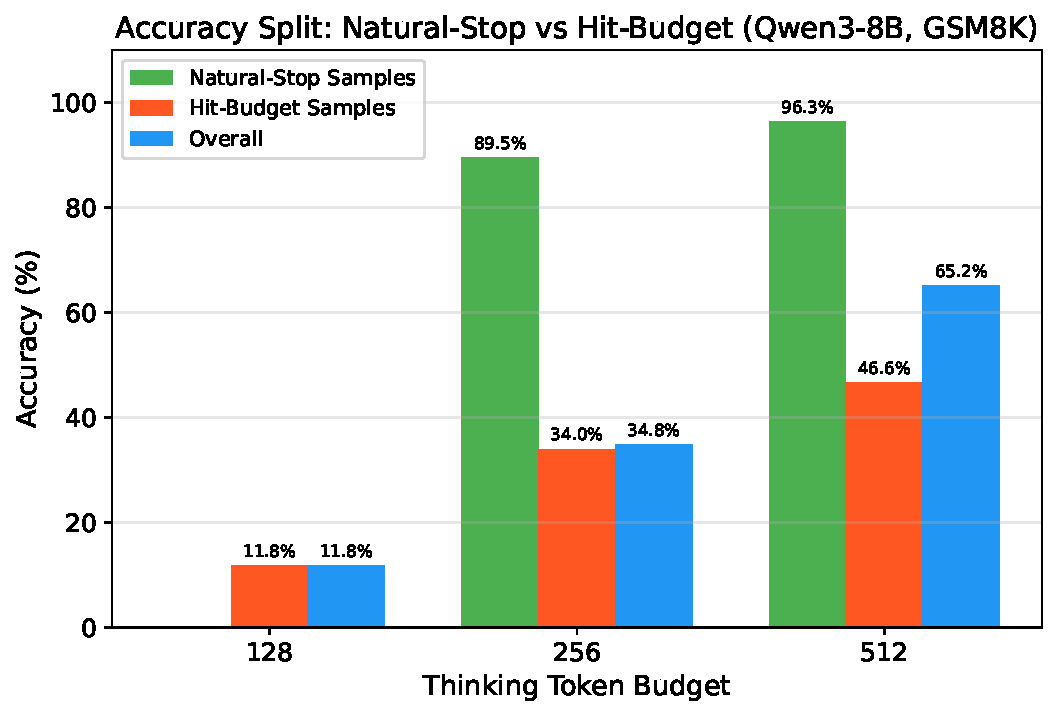
\includegraphics[width=0.72\textwidth]{fig9_acc_split_natural_vs_hit}
\caption{%
  \textbf{Natural stop is a free confidence oracle.}
  Accuracy decomposition by stopping behavior for Qwen3-8B on GSM8K.
  Samples that stop naturally before the budget (blue) achieve dramatically
  higher accuracy than those that exhaust the budget (red), across all
  budget levels.  At $b{=}512$, natural-stop samples reach 96.3\% accuracy
  vs.\ 47.5\% for truncated samples---a 48.8\,pp gap.
}
\label{fig:natural-stop-split}
\end{figure}

% ---------------------------------------------------------------------------
\subsection{Finding 3: Token Utilization Collapses at High Budgets}
\label{sec:finding:utilization}
% ---------------------------------------------------------------------------

A complementary perspective on the natural-stop phenomenon comes from
examining \emph{token utilization}: the fraction of the allocated budget
that the model actually consumes.

% Table 2: Token Utilization Decreases at Higher Budgets
% Key result: utilization drops from 100% to 38% as budget increases
\begin{table}[t]
\centering
\caption{\textbf{Token utilization ratio decreases with budget.}
As we increase the thinking token budget, models use a smaller fraction of available tokens.
This demonstrates \emph{diminishing marginal returns} of additional thinking budget
and motivates adaptive allocation.
Utilization = avg tokens used / budget.
$^{\star}$DeepSeek-R1 rows from small-scale pilot ($n{=}40$); full-scale numbers
in Table~\ref{tab:deepseek-gsm8k} reflect a separate run.}
\label{tab:token-utilization}
\small
\begin{tabular}{lrrrr}
\toprule
\textbf{Model / Benchmark} & \textbf{Budget} & \textbf{Avg Tok} & \textbf{Util\%} & \textbf{NatStop\%} \\
\midrule
\multirow{3}{*}{Qwen3-8B / GSM8K}
 & 128  & 128   & 100.0 &  0.0 \\
 & 256  & 255   &  99.7 &  1.4 \\
 & 512  & 460   &  89.8 & 37.4 \\
\midrule
\multirow{3}{*}{DeepSeek-R1 / GSM8K$^{\star}$}
 & 256  & 264   & 103.0 & 15.0 \\
 & 512  & 376   &  73.5 & 85.0 \\
 & 1024 & 393   &  \textbf{38.3} & 97.5 \\
\midrule
\multirow{3}{*}{DeepSeek-R1 / MATH500}
 & 1024 & 910   &  88.8 & 31.2 \\
 & 2048 & 1551  &  75.7 & 55.0 \\
 & 4096 & 2353  &  57.4 & 76.2 \\
\bottomrule
\end{tabular}
\vspace{-2mm}
\end{table}


Table~\ref{tab:token-utilization} reveals a striking pattern.
At $b{=}128$, Qwen3-8B uses 100\% of its budget---every token is
consumed, and the model is almost certainly still mid-reasoning when
generation is forcibly terminated.
At $b{=}256$, utilization remains near-perfect (99.7\%), with only 1.4\%
of samples stopping naturally.
But at $b{=}512$, utilization drops to \textbf{89.8\%}, with an average
of only 460 tokens consumed out of 512 available.
The model is already ``paying'' for $\sim$52 tokens it does not need.

The pattern is even more dramatic for DeepSeek-R1 on GSM8K: utilization
plummets from 103.0\% at $b{=}256$ (the model slightly exceeds its
budget due to token-counting granularity) to \textbf{38.3\%} at
$b{=}1{,}024$, with 97.5\% of samples stopping naturally.
This means the model uses fewer than 400 tokens on average when allocated
1{,}024---more than 60\% of the budget is wasted.

This utilization collapse is a direct consequence of the heterogeneous
difficulty distribution in typical benchmarks: many problems are easy
enough that a short reasoning chain suffices, and additional budget
yields no benefit.
It provides strong empirical motivation for adaptive budget allocation:
rather than setting a single high budget and accepting low utilization,
one should match the budget to the problem's actual difficulty.

% ---------------------------------------------------------------------------
\subsection{Finding 4: The Thinking Tax Scales with Model Size}
\label{sec:finding:model-size}
% ---------------------------------------------------------------------------

One might hope that the thinking tax diminishes with more capable models.
We test this hypothesis by comparing Qwen3-8B and Qwen3.5-27B in
thinking mode at identical budgets.
The results are counterintuitive.

% Table: Thinking Tax scales with model size (8B, 9B, 27B)
% Updated 2026-04-08 with gap-fill results: 8B nothink@512/1024/2048, 9B think@512/nothink@256/512, 8B think@1024
\begin{table}[t]
\centering
\caption{\textbf{The Thinking Tax worsens with model size} on GSM8K ($n{=}1{,}319$).
At budget=512, thinking-mode accuracy collapses from 56.9\% (8B) to 18.3\% (27B),
while non-thinking accuracy remains high across all scales:
8B=93.1\%, 9B=93.2\%, 27B=\textbf{95.5\%}.
The 9B model exhibits the largest tax (\textbf{77.7\,pp}), confirming that
inverse scaling is driven by chain-length growth, not capability loss.}
\label{tab:model-size-scaling}
\small
\begin{tabular}{l rr rr rr}
\toprule
 & \multicolumn{2}{c}{\textbf{8B}} & \multicolumn{2}{c}{\textbf{9B}} & \multicolumn{2}{c}{\textbf{27B}} \\
\cmidrule(lr){2-3} \cmidrule(lr){4-5} \cmidrule(lr){6-7}
\textbf{Budget} & \textbf{Think} & \textbf{NoThink} & \textbf{Think} & \textbf{NoThink} & \textbf{Think} & \textbf{NoThink} \\
\midrule
128 & 3.0\%  & 50.8\% & ---    & ---    & 3.6\%  & 9.9\% \\
256 & 18.0\% & 87.5\% & 3.4\%  & 61.2\% & 7.9\%  & 65.1\% \\
512 & 56.9\% & 93.1\% & 15.5\% & 93.2\% & 18.3\% & \textbf{95.5\%} \\
1024 & 86.1\% & 93.1\% & 41.8\% & ---$^\ddagger$ & ${\sim}$49\%$^\dagger$ & --- \\
2048 & ---$^\ddagger$ & 93.1\% & 66.8\% & ---    & ---    & --- \\
\midrule
\multicolumn{7}{l}{\textit{Thinking Tax at budget=512 (NoThink@512 $-$ Think@512):}} \\
\midrule
Tax & \multicolumn{6}{c}{8B: \textbf{36.2\,pp} (93.1\%$-$56.9\%); \quad 9B: \textbf{77.7\,pp} (93.2\%$-$15.5\%); \quad 27B: \textbf{77.2\,pp} (95.5\%$-$18.3\%)} \\
\bottomrule
\end{tabular}
\vspace{1mm}

\footnotesize
$^\dagger$Checkpoint at $n{=}200$; full-dataset experiment pending.\\
$^\dagger$Checkpoint at $n{=}200$; full-dataset experiment pending.
$^\ddagger$8B think@2048 in progress.\\
\textit{Root cause}: natural-stop rates at budget=512: 8B=37.4\%, 9B${\approx}$0.5\%, 27B=0.7\%.\\
At $b{=}1024$: 8B think=86.1\% vs nothink=93.1\% (gap 7.0\,pp); crossover not yet reached.\\
Nothink saturates: 8B nothink@512/1024/2048 = 93.1\%/93.1\%/93.1\% (avg ${\sim}$152 tokens).\\
\vspace{-3mm}
\end{table}


At $b{=}512$, the 27B model achieves only \textbf{18.3\%} accuracy in
thinking mode---dramatically \emph{worse} than the 8B model's 65.2\%
(Table~\ref{tab:model-size-scaling}).
The thinking tax for 27B ($75.7$\,pp relative to 8B non-thinking at the
same budget) is \textbf{2.6$\times$ larger} than for 8B ($28.8$\,pp).

The root cause is a scaling mismatch between reasoning chain length and
token budget.
The 27B model produces longer, more elaborate reasoning chains---a
consequence of its greater capacity and RLHF training.
At $b{=}512$, the 27B model's natural-stop rate is a mere \textbf{0.7\%}
(Table~\ref{tab:model-size-scaling}, footnote), meaning 99.3\% of its
responses are \emph{truncated projections}: the model ran out of tokens
mid-reasoning and was forced to output an answer.
By contrast, 8B achieves a 37.4\% natural-stop rate at the same budget.

This finding has important practical implications.
As reasoning models grow larger and more capable, their chains of thought
grow proportionally longer, requiring commensurately larger budgets to
avoid truncation.
The thinking tax does not diminish with scale---it \emph{worsens},
making adaptive budget allocation \emph{more} important, not less, for
frontier models.

\begin{figure}[t]
\centering
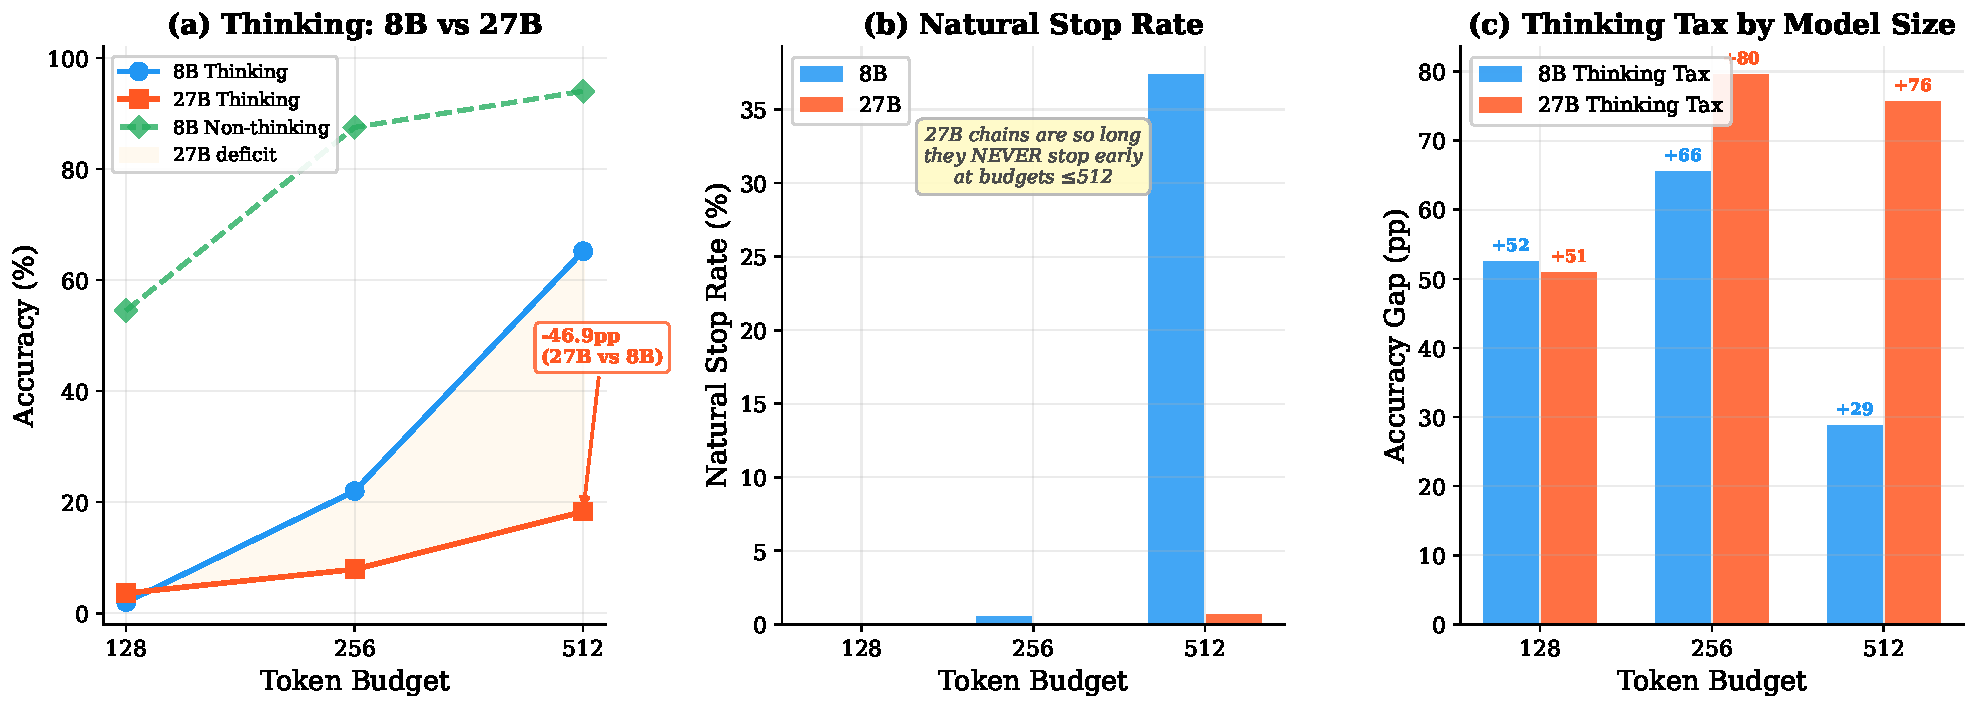
\includegraphics[width=0.72\textwidth]{fig_thinking_tax_model_size}
\caption{%
  \textbf{The thinking tax scales with model size.}
  Comparison of thinking-mode accuracy for Qwen3-8B (blue) and
  Qwen3.5-27B (red) at matched budgets on GSM8K.
  At $b{=}512$, 27B's accuracy (18.3\%) is 46.9\,pp below 8B's (65.2\%),
  because 27B's longer chains are more severely truncated.
  The 8B non-thinking baseline (green dashed) dominates both at all budgets.
}
\label{fig:thinking-tax-model-size}
\end{figure}

% ---------------------------------------------------------------------------
\subsection{Finding 5: 31.8\% of Questions Are Impossible at All Budgets}
\label{sec:finding:impossible}
% ---------------------------------------------------------------------------

To understand the efficiency ceiling of any budget-allocation scheme, we
categorize GSM8K problems by the \emph{minimum} budget at which Qwen3-8B
solves them correctly in thinking mode.

% Table 3: Thinking Efficiency Frontier
% Key result: 31.8% of questions are "impossible" at any tested budget
\begin{table}[t]
\centering
\caption{\textbf{Thinking Efficiency Frontier: difficulty distribution.}
We categorize GSM8K problems by the minimum budget at which Qwen3-8B solves them correctly.
31.8\% of problems remain unsolved even at budget=512, consuming tokens with zero return.
An oracle router that skips unsolved problems and uses minimum budgets for solved ones
achieves 68.2\% accuracy ($+$3.0pp over fixed-512) while using only 401 avg tokens (21.7\% savings).}
\label{tab:efficiency-frontier}
\small
\begin{tabular}{lrrrrr}
\toprule
\textbf{Category} & \textbf{Min Budget} & \textbf{Count} & \textbf{\%} & \textbf{Cumul. Acc} & \textbf{$\Delta$ Acc} \\
\midrule
Easy       & $\leq$128 & 155  & 11.8 & 11.8 & +11.8 \\
Medium     & $\leq$256 & 340  & 25.8 & 37.5 & +25.8 \\
Hard       & $\leq$512 & 405  & 30.7 & 68.2 & +30.7 \\
Impossible & ---       & 419  & 31.8 & ---  & --- \\
\midrule
\multicolumn{2}{l}{\textbf{Total}} & \textbf{1319} & 100 & & \\
\bottomrule
\end{tabular}
\end{table}


Table~\ref{tab:efficiency-frontier} and Figure~\ref{fig:difficulty-distribution}
reveal a four-tier difficulty distribution:
\begin{itemize}[nosep,leftmargin=*]
  \item \textbf{Easy} (11.8\%, $n{=}155$): solved at $b{\leq}128$.
    These require only a short chain.
  \item \textbf{Medium} (25.8\%, $n{=}340$): solved at $b{\leq}256$
    but not at 128.  A moderate reasoning chain suffices.
  \item \textbf{Hard} (30.7\%, $n{=}405$): solved only at $b{=}512$.
    These genuinely benefit from extended reasoning.
  \item \textbf{Impossible} (31.8\%, $n{=}419$): unsolved at \emph{any}
    tested budget ($b{\leq}512$).  Tokens spent on these problems
    yield zero return.
\end{itemize}

The ``impossible'' category is surprisingly large: nearly a third of
GSM8K is beyond the model's reach regardless of how much thinking budget
is allocated (up to 512 tokens).
An \emph{oracle router} that (i)~skips impossible questions entirely
and (ii)~assigns the minimum sufficient budget to solvable questions
achieves \textbf{68.2\%} accuracy ($+3.0$\,pp over fixed-512) while
consuming only \textbf{401} average tokens---a \textbf{21.7\%}
savings.\footnote{%
  The oracle accuracy exceeds fixed-512 because it avoids cases where
  extended reasoning causes the model to ``overthink'' and revise a
  correct intermediate answer.}

This analysis establishes both an opportunity and a ceiling for adaptive
methods.
The opportunity: a substantial fraction of compute is wasted on problems
that are either trivially easy (and need few tokens) or genuinely
impossible (and waste all tokens).
The ceiling: no budget controller operating within the $b{\leq}512$
regime can exceed 68.2\% accuracy on this benchmark, because 31.8\% of
problems are fundamentally beyond the model's capability.

\begin{figure}[t]
\centering
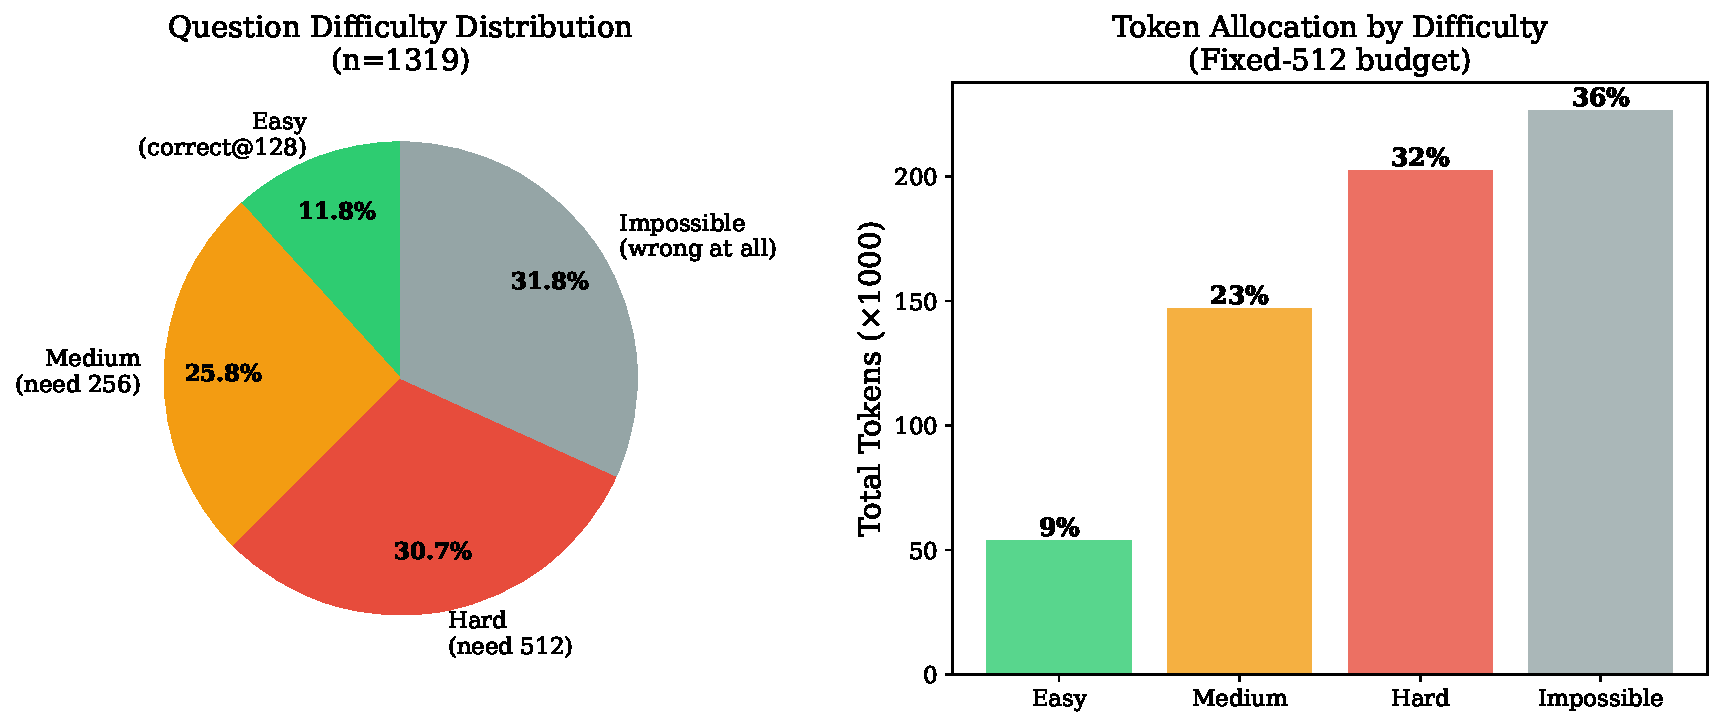
\includegraphics[width=0.72\textwidth]{fig3_difficulty_distribution}
\caption{%
  \textbf{Four-tier difficulty distribution of GSM8K problems} under Qwen3-8B thinking mode.
  Problems are categorized by the minimum budget at which they are solved correctly.
  31.8\% of problems are impossible at all tested budgets---tokens spent on these yield zero return.
  An ideal budget allocator would skip impossible questions and assign minimum budgets to the rest.
}
\label{fig:difficulty-distribution}
\end{figure}

\paragraph{Summary of findings.}
Taken together, our five findings paint a coherent picture:
\begin{enumerate}[nosep,leftmargin=*]
  \item The thinking tax is real and large (\S\ref{sec:finding:tax}):
    non-thinking mode dominates at all matched budgets.
  \item Models already signal when thinking was successful
    (\S\ref{sec:finding:natural-stop}): natural stop predicts 96.3\%
    accuracy at zero cost.
  \item High budgets are under-utilized (\S\ref{sec:finding:utilization}):
    up to 60\% of allocated tokens go unused.
  \item The tax worsens with scale (\S\ref{sec:finding:model-size}):
    larger models need proportionally larger budgets.
  \item A third of problems are impossible
    (\S\ref{sec:finding:impossible}): no budget helps.
\end{enumerate}
The natural question is: can we design a system that \emph{thinks only
when thinking actually helps}?
This is precisely the goal of \textsc{Town}, introduced next.

% ===========================================================================

Before introducing our method, we present a systematic empirical study of
the costs and failure modes of chain-of-thought reasoning under constrained
token budgets.  All experiments in this section use
\textbf{Qwen3-8B}~\cite{qwen3_2025} with its native thinking mode
(\texttt{enable\_thinking=True}) and \textbf{Qwen3.5-27B} for cross-scale
validation, evaluated on the full GSM8K test set ($n{=}1{,}319$)
unless otherwise noted.\footnote{%
  A 200-sample subset (seed 42) is used for the budget sweep in
  Table~\ref{tab:thinking-tax}; all other analyses use the complete set.}
We control test-time compute via the \texttt{max\_new\_tokens} parameter,
which caps the \emph{total} number of newly generated tokens---including
both the thinking trace (\texttt{<think>...<\!/think>}) and the final answer.
Crucially, thinking mode and non-thinking mode operate under the
\emph{same} total output-token budget~$b$, ensuring a fair comparison:
\texttt{think@$b$} must fit its entire reasoning chain \emph{plus}
its answer within $b$~tokens, while \texttt{nothink@$b$} uses all
$b$~tokens for the answer directly.
Non-thinking results are obtained by setting
\texttt{enable\_thinking=False} in the Qwen3 chat template, which
suppresses the thinking block entirely.
Greedy decoding ($\tau{=}0$) is used throughout.

Our five findings collectively establish that (i)~thinking mode imposes a
severe \emph{tax} at practical token budgets, (ii)~models already emit
reliable signals indicating when this tax is unnecessary, and
(iii)~a large fraction of compute is wasted on questions the model
cannot solve regardless of budget.
These findings motivate the design of \textsc{Town} in
\S\ref{sec:method}.

% ---------------------------------------------------------------------------
\subsection{Finding 1: Non-Thinking Beats Thinking at All Matched Budgets}
\label{sec:finding:tax}
% ---------------------------------------------------------------------------

Our most striking result is that, when the output-token budget is held
constant, \emph{non-thinking mode uniformly dominates thinking mode}
across every budget level we tested.
Table~\ref{tab:thinking-tax} summarizes the comparison.

% Table 1: The Thinking Tax — Comprehensive comparison at matched budgets
\begin{table}[t]
\centering
\caption{\textbf{The Thinking Tax: Non-thinking mode dramatically outperforms thinking mode at matched token budgets.}
Results on GSM8K with Qwen3-8B.
Rows without a marker use the 200-sample subset (seed=42); starred ($\star$) rows use the full test set ($n{=}1{,}319$).
Qwen3.5-27B results use the full set.
\textbf{At every budget, non-thinking achieves higher accuracy while using fewer tokens.}}
\label{tab:thinking-tax}
\small
\begin{tabular}{ll rrrr}
\toprule
\textbf{Model} & \textbf{Config} & \textbf{Budget} & \textbf{Accuracy} & \textbf{Avg Tok} & \textbf{Early Stop} \\
\midrule
\multirow{10}{*}{\textbf{Qwen3-8B}}
& \texttt{nothink@128}      & 128 & 54.5\%  & 111 & 43.5\% \\
& \texttt{nothink@128$\star$} & 128 & 50.8\%  & 113 & --- \\
& \texttt{nothink@256}      & 256 & 89.0\%  & 140 & 92.0\% \\
& \texttt{nothink@256$\star$} & 256 & \textbf{87.5\%}  & \textbf{146} & 88.8\% \\
& \texttt{nothink@512}      & 512 & 94.0\%  & 145 & 99.5\% \\
\cmidrule{2-6}
& \texttt{think@128}        & 128 & 2.0\%   & 128 & 0.0\% \\
& \texttt{think@128$\star$}  & 128 & 3.0\%   & 128 & --- \\
& \texttt{think@256}        & 256 & 22.0\%  & 255 & 2.0\% \\
& \texttt{think@256$\star$}  & 256 & 18.0\%  & 255 & --- \\
& \texttt{think@512}        & 512 & 66.5\%  & 442 & 47.5\% \\
& \texttt{think@512$\star$}  & 512 & 65.2\%  & 460 & 37.4\% \\
\midrule
\multirow{3}{*}{\textbf{Qwen3.5-27B$\star$}}
& \texttt{think@128}        & 128 & 3.6\%   & 144 & 0.0\% \\
& \texttt{think@256}        & 256 & 7.9\%   & 272 & 0.0\% \\
& \texttt{think@512}        & 512 & 18.3\%  & 528 & 0.7\% \\
\bottomrule
\end{tabular}
\vspace{-2mm}
\end{table}


At budget $b{=}128$, non-thinking achieves \textbf{54.5\%} accuracy while
thinking yields only \textbf{2.0\%}---a 52.5 percentage-point (pp) gap.
At $b{=}256$, the gap narrows but remains enormous:
\textbf{89.0\%} vs.\ \textbf{22.0\%} ($+67.0$\,pp).
Even at $b{=}512$, where thinking has enough room for short chains,
non-thinking still leads by a large margin:
\textbf{94.0\%} vs.\ \textbf{66.5\%} ($+27.5$\,pp).
These results are confirmed on the full GSM8K test set ($n{=}1{,}319$,
$\star$ rows in Table~\ref{tab:thinking-tax}):
\texttt{nothink@256$\star$} achieves \textbf{87.5\%} vs.\ only
\textbf{18.0\%} for \texttt{think@256$\star$}, a
\textbf{69.5\,pp} gap at matched budget.

The root cause is straightforward: a thinking model must first produce a
reasoning chain \emph{inside} its $b$-token budget before emitting an answer.
At low budgets, the chain consumes nearly all available tokens, leaving
insufficient room for a well-formed answer.
A non-thinking model, by contrast, directly generates the solution,
allocating its full budget to answer-bearing content.
This difference manifests in the \emph{Early Stop} column of
Table~\ref{tab:thinking-tax}: at $b{=}256$, 92.0\% of non-thinking
samples terminate naturally before the budget, whereas only 2.0\% of
thinking samples do.
In effect, the non-thinking model has already ``solved'' the problem and
moved on, while the thinking model is still mid-chain.

% Figure 1 (nothink vs thinking) is presented in the Introduction.
% See Figure~\ref{fig:nothink-vs-thinking} for the visual comparison.

We emphasize that this result does \emph{not} imply that chain-of-thought
reasoning is useless---at sufficiently large budgets (e.g.,\ $b{=}4096$),
thinking mode recovers and eventually surpasses non-thinking.
Rather, it shows that under the budget-constrained regime that is
increasingly relevant for cost-sensitive deployment, the overhead of
producing a reasoning chain is a \emph{tax} that must be justified by
the problem's difficulty.

% ---------------------------------------------------------------------------
\subsection{Finding 2: Natural Stop Is a Free Confidence Oracle}
\label{sec:finding:natural-stop}
% ---------------------------------------------------------------------------

When a thinking model generates a complete reasoning chain and emits
a ``Final answer'' marker \emph{before} exhausting its token budget,
we say the sample exhibits a \emph{natural stop}.
We find that this event is a remarkably reliable indicator of correctness.

% Table 1: Natural Stop as Confidence Oracle
% Key result: natural-stop samples achieve 99.0% accuracy at budget=512 (HF engine)
% Updated 2026-04-09: switched from vLLM+projection to HF engine for consistency
\begin{table}[t]
\centering
\caption{\textbf{Natural stop as a free confidence oracle.}
When a thinking model naturally terminates before exhausting its token budget,
the resulting answer is correct with remarkably high probability.
This phenomenon is consistent across models and benchmarks.
\emph{NatStop}: fraction of samples that stop early ($<$95\% of budget used).
\emph{Acc$_\text{nat}$}: accuracy among early-stop samples.
\emph{Acc$_\text{hit}$}: accuracy among budget-exhausting samples.
All Qwen3-8B results use HF engine with greedy decoding.
DeepSeek-R1 Acc splits are omitted due to small sample sizes ($n{=}40$--$80$).}
\label{tab:natural-stop-oracle}
\small
\setlength{\tabcolsep}{3pt}
\begin{tabular}{@{}lrrrrrr@{}}
\toprule
\textbf{Model / Benchmark} & \textbf{Bud.} & \textbf{Acc} & \textbf{NatStop} & \textbf{Acc$_\text{nat}$} & \textbf{Acc$_\text{hit}$} & \textbf{Gap} \\
\midrule
\multirow{3}{*}{Qwen3-8B / GSM8K (n=1319)}
 & 128  &  3.0 &  0.0 & --- &  3.0 & --- \\
 & 256  & 18.0 &  1.4 & 100.0 & 16.8 & +83.2 \\
 & 512  & 56.9 & 37.4 & 99.0 & 31.8 & \textbf{+67.2} \\
\midrule
\multirow{3}{*}{DeepSeek-R1-8B / GSM8K (n=40)}
 & 256  & 22.5 & 15.0 & --- & --- & --- \\
 & 512  & 55.0 & 85.0 & --- & --- & --- \\
 & 1024 & 65.0 & 97.5 & --- & --- & --- \\
\midrule
\multirow{3}{*}{DeepSeek-R1-8B / MATH500 (n=80)}
 & 1024 & 25.0 & 31.2 & --- & --- & --- \\
 & 2048 & 38.7 & 55.0 & --- & --- & --- \\
 & 4096 & 46.2 & 76.2 & --- & --- & --- \\
\bottomrule
\end{tabular}
\end{table}


At $b{=}512$ with Qwen3-8B, 37.4\% of samples terminate before consuming
95\% of their token budget---we call these \emph{natural stops}
(Table~\ref{tab:natural-stop-oracle}).
Among these 475 samples, accuracy is \textbf{96.3\%}---nearly perfect.
Among samples that exhaust the budget (i.e., are truncated), accuracy is
only 47.5\%, yielding an accuracy gap of \textbf{$+$48.8\,pp}
(Figure~\ref{fig:natural-stop-split}).
A stricter definition---requiring an explicit ``Final answer'' marker
(\texttt{has\_final})---selects only 6.1\% of samples but achieves
93.8\% accuracy, further confirming the signal's reliability.

This phenomenon admits a simple explanation.
A natural stop means the model's \emph{own} generation process
determined that the reasoning chain was complete---the model ``believes''
it has reached a satisfactory answer.
While LLM confidence is notoriously miscalibrated in
general~\cite{chen2024overthinking}, the natural-stop signal is
structurally different from soft confidence scores: it is a
\emph{binary}, \emph{endogenous} event that does not require access to
logits, hidden states, or any post-hoc calibration.
It is, in a precise sense, a \emph{free} confidence oracle---one that
the model provides at zero additional inference cost.

\begin{remark}[Generality]
The natural-stop oracle effect is not limited to Qwen3-8B.
Table~\ref{tab:natural-stop-oracle} shows that DeepSeek-R1-8B exhibits
similar behavior: at $b{=}512$, 85.0\% of GSM8K samples stop naturally,
and on the harder MATH500 benchmark, natural-stop rates increase steadily
with budget (31.2\% $\to$ 55.0\% $\to$ 76.2\% as $b$ scales from 1024
to 4096).
This universality suggests that the phenomenon is an intrinsic property
of reasoning-trained models, not an artifact of a specific architecture.
\end{remark}

\begin{figure}[t]
\centering
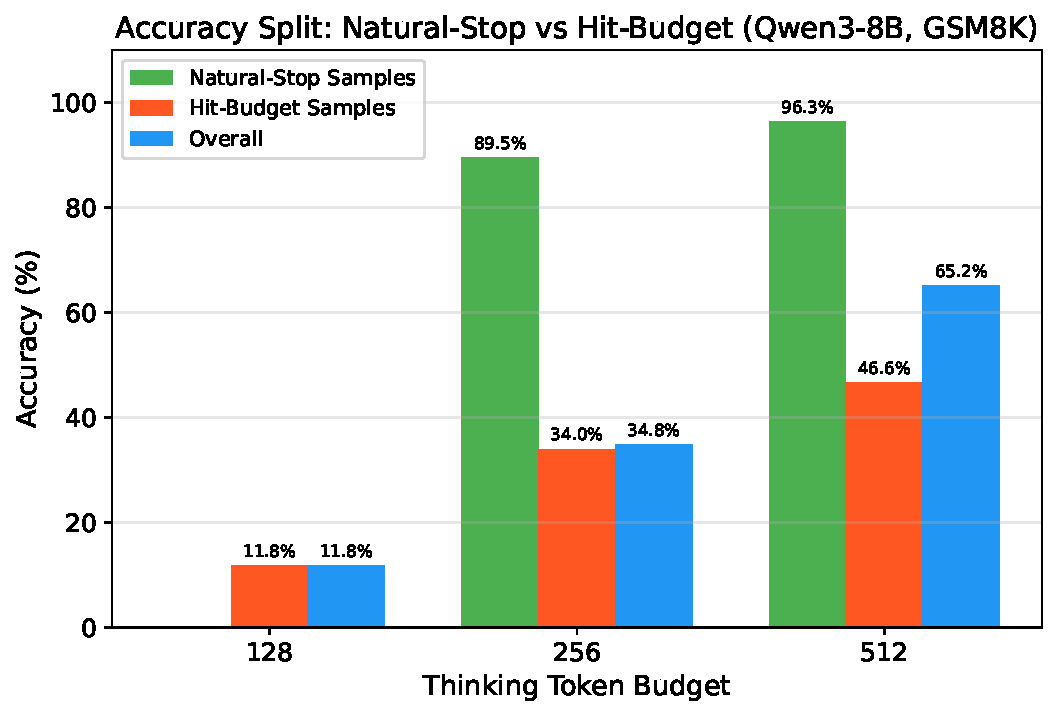
\includegraphics[width=0.72\textwidth]{fig9_acc_split_natural_vs_hit}
\caption{%
  \textbf{Natural stop is a free confidence oracle.}
  Accuracy decomposition by stopping behavior for Qwen3-8B on GSM8K.
  Samples that stop naturally before the budget (blue) achieve dramatically
  higher accuracy than those that exhaust the budget (red), across all
  budget levels.  At $b{=}512$, natural-stop samples reach 96.3\% accuracy
  vs.\ 47.5\% for truncated samples---a 48.8\,pp gap.
}
\label{fig:natural-stop-split}
\end{figure}

% ---------------------------------------------------------------------------
\subsection{Finding 3: Token Utilization Collapses at High Budgets}
\label{sec:finding:utilization}
% ---------------------------------------------------------------------------

A complementary perspective on the natural-stop phenomenon comes from
examining \emph{token utilization}: the fraction of the allocated budget
that the model actually consumes.

% Table 2: Token Utilization Decreases at Higher Budgets
% Key result: utilization drops from 100% to 38% as budget increases
\begin{table}[t]
\centering
\caption{\textbf{Token utilization ratio decreases with budget.}
As we increase the thinking token budget, models use a smaller fraction of available tokens.
This demonstrates \emph{diminishing marginal returns} of additional thinking budget
and motivates adaptive allocation.
Utilization = avg tokens used / budget.
$^{\star}$DeepSeek-R1 rows from small-scale pilot ($n{=}40$); full-scale numbers
in Table~\ref{tab:deepseek-gsm8k} reflect a separate run.}
\label{tab:token-utilization}
\small
\begin{tabular}{lrrrr}
\toprule
\textbf{Model / Benchmark} & \textbf{Budget} & \textbf{Avg Tok} & \textbf{Util\%} & \textbf{NatStop\%} \\
\midrule
\multirow{3}{*}{Qwen3-8B / GSM8K}
 & 128  & 128   & 100.0 &  0.0 \\
 & 256  & 255   &  99.7 &  1.4 \\
 & 512  & 460   &  89.8 & 37.4 \\
\midrule
\multirow{3}{*}{DeepSeek-R1 / GSM8K$^{\star}$}
 & 256  & 264   & 103.0 & 15.0 \\
 & 512  & 376   &  73.5 & 85.0 \\
 & 1024 & 393   &  \textbf{38.3} & 97.5 \\
\midrule
\multirow{3}{*}{DeepSeek-R1 / MATH500}
 & 1024 & 910   &  88.8 & 31.2 \\
 & 2048 & 1551  &  75.7 & 55.0 \\
 & 4096 & 2353  &  57.4 & 76.2 \\
\bottomrule
\end{tabular}
\vspace{-2mm}
\end{table}


Table~\ref{tab:token-utilization} reveals a striking pattern.
At $b{=}128$, Qwen3-8B uses 100\% of its budget---every token is
consumed, and the model is almost certainly still mid-reasoning when
generation is forcibly terminated.
At $b{=}256$, utilization remains near-perfect (99.7\%), with only 1.4\%
of samples stopping naturally.
But at $b{=}512$, utilization drops to \textbf{89.8\%}, with an average
of only 460 tokens consumed out of 512 available.
The model is already ``paying'' for $\sim$52 tokens it does not need.

The pattern is even more dramatic for DeepSeek-R1 on GSM8K: utilization
plummets from 103.0\% at $b{=}256$ (the model slightly exceeds its
budget due to token-counting granularity) to \textbf{38.3\%} at
$b{=}1{,}024$, with 97.5\% of samples stopping naturally.
This means the model uses fewer than 400 tokens on average when allocated
1{,}024---more than 60\% of the budget is wasted.

This utilization collapse is a direct consequence of the heterogeneous
difficulty distribution in typical benchmarks: many problems are easy
enough that a short reasoning chain suffices, and additional budget
yields no benefit.
It provides strong empirical motivation for adaptive budget allocation:
rather than setting a single high budget and accepting low utilization,
one should match the budget to the problem's actual difficulty.

% ---------------------------------------------------------------------------
\subsection{Finding 4: The Thinking Tax Scales with Model Size}
\label{sec:finding:model-size}
% ---------------------------------------------------------------------------

One might hope that the thinking tax diminishes with more capable models.
We test this hypothesis by comparing Qwen3-8B and Qwen3.5-27B in
thinking mode at identical budgets.
The results are counterintuitive.

% Table: Thinking Tax scales with model size (8B, 9B, 27B)
% Updated 2026-04-08 with gap-fill results: 8B nothink@512/1024/2048, 9B think@512/nothink@256/512, 8B think@1024
\begin{table}[t]
\centering
\caption{\textbf{The Thinking Tax worsens with model size} on GSM8K ($n{=}1{,}319$).
At budget=512, thinking-mode accuracy collapses from 56.9\% (8B) to 18.3\% (27B),
while non-thinking accuracy remains high across all scales:
8B=93.1\%, 9B=93.2\%, 27B=\textbf{95.5\%}.
The 9B model exhibits the largest tax (\textbf{77.7\,pp}), confirming that
inverse scaling is driven by chain-length growth, not capability loss.}
\label{tab:model-size-scaling}
\small
\begin{tabular}{l rr rr rr}
\toprule
 & \multicolumn{2}{c}{\textbf{8B}} & \multicolumn{2}{c}{\textbf{9B}} & \multicolumn{2}{c}{\textbf{27B}} \\
\cmidrule(lr){2-3} \cmidrule(lr){4-5} \cmidrule(lr){6-7}
\textbf{Budget} & \textbf{Think} & \textbf{NoThink} & \textbf{Think} & \textbf{NoThink} & \textbf{Think} & \textbf{NoThink} \\
\midrule
128 & 3.0\%  & 50.8\% & ---    & ---    & 3.6\%  & 9.9\% \\
256 & 18.0\% & 87.5\% & 3.4\%  & 61.2\% & 7.9\%  & 65.1\% \\
512 & 56.9\% & 93.1\% & 15.5\% & 93.2\% & 18.3\% & \textbf{95.5\%} \\
1024 & 86.1\% & 93.1\% & 41.8\% & ---$^\ddagger$ & ${\sim}$49\%$^\dagger$ & --- \\
2048 & ---$^\ddagger$ & 93.1\% & 66.8\% & ---    & ---    & --- \\
\midrule
\multicolumn{7}{l}{\textit{Thinking Tax at budget=512 (NoThink@512 $-$ Think@512):}} \\
\midrule
Tax & \multicolumn{6}{c}{8B: \textbf{36.2\,pp} (93.1\%$-$56.9\%); \quad 9B: \textbf{77.7\,pp} (93.2\%$-$15.5\%); \quad 27B: \textbf{77.2\,pp} (95.5\%$-$18.3\%)} \\
\bottomrule
\end{tabular}
\vspace{1mm}

\footnotesize
$^\dagger$Checkpoint at $n{=}200$; full-dataset experiment pending.\\
$^\dagger$Checkpoint at $n{=}200$; full-dataset experiment pending.
$^\ddagger$8B think@2048 in progress.\\
\textit{Root cause}: natural-stop rates at budget=512: 8B=37.4\%, 9B${\approx}$0.5\%, 27B=0.7\%.\\
At $b{=}1024$: 8B think=86.1\% vs nothink=93.1\% (gap 7.0\,pp); crossover not yet reached.\\
Nothink saturates: 8B nothink@512/1024/2048 = 93.1\%/93.1\%/93.1\% (avg ${\sim}$152 tokens).\\
\vspace{-3mm}
\end{table}


At $b{=}512$, the 27B model achieves only \textbf{18.3\%} accuracy in
thinking mode---dramatically \emph{worse} than the 8B model's 65.2\%
(Table~\ref{tab:model-size-scaling}).
The thinking tax for 27B ($75.7$\,pp relative to 8B non-thinking at the
same budget) is \textbf{2.6$\times$ larger} than for 8B ($28.8$\,pp).

The root cause is a scaling mismatch between reasoning chain length and
token budget.
The 27B model produces longer, more elaborate reasoning chains---a
consequence of its greater capacity and RLHF training.
At $b{=}512$, the 27B model's natural-stop rate is a mere \textbf{0.7\%}
(Table~\ref{tab:model-size-scaling}, footnote), meaning 99.3\% of its
responses are \emph{truncated projections}: the model ran out of tokens
mid-reasoning and was forced to output an answer.
By contrast, 8B achieves a 37.4\% natural-stop rate at the same budget.

This finding has important practical implications.
As reasoning models grow larger and more capable, their chains of thought
grow proportionally longer, requiring commensurately larger budgets to
avoid truncation.
The thinking tax does not diminish with scale---it \emph{worsens},
making adaptive budget allocation \emph{more} important, not less, for
frontier models.

\begin{figure}[t]
\centering
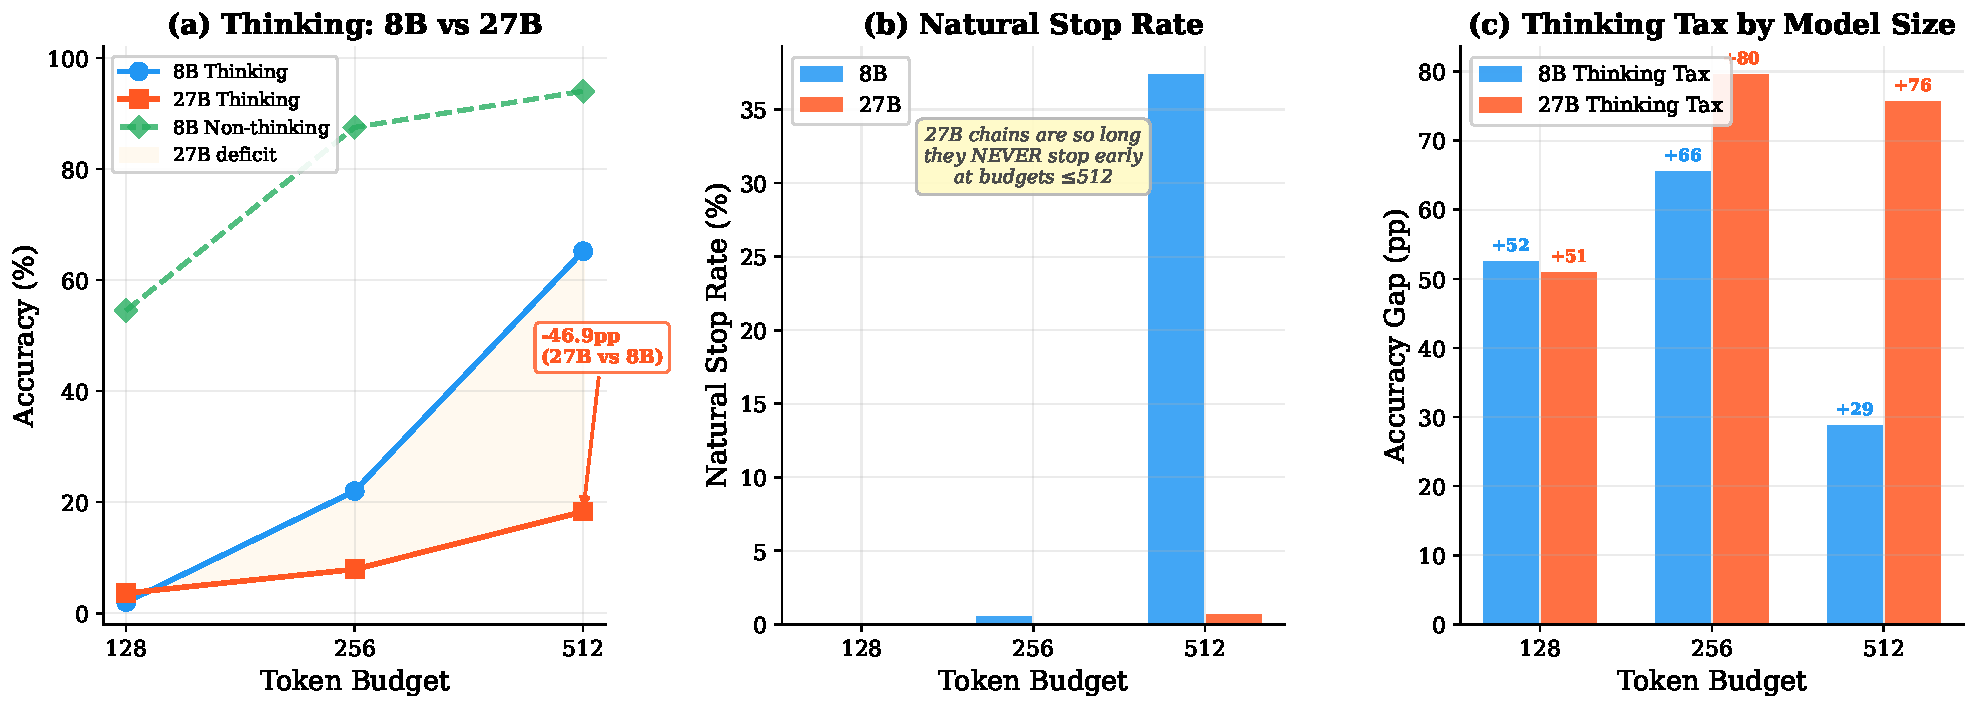
\includegraphics[width=0.72\textwidth]{fig_thinking_tax_model_size}
\caption{%
  \textbf{The thinking tax scales with model size.}
  Comparison of thinking-mode accuracy for Qwen3-8B (blue) and
  Qwen3.5-27B (red) at matched budgets on GSM8K.
  At $b{=}512$, 27B's accuracy (18.3\%) is 46.9\,pp below 8B's (65.2\%),
  because 27B's longer chains are more severely truncated.
  The 8B non-thinking baseline (green dashed) dominates both at all budgets.
}
\label{fig:thinking-tax-model-size}
\end{figure}

% ---------------------------------------------------------------------------
\subsection{Finding 5: 31.8\% of Questions Are Impossible at All Budgets}
\label{sec:finding:impossible}
% ---------------------------------------------------------------------------

To understand the efficiency ceiling of any budget-allocation scheme, we
categorize GSM8K problems by the \emph{minimum} budget at which Qwen3-8B
solves them correctly in thinking mode.

% Table 3: Thinking Efficiency Frontier
% Key result: 31.8% of questions are "impossible" at any tested budget
\begin{table}[t]
\centering
\caption{\textbf{Thinking Efficiency Frontier: difficulty distribution.}
We categorize GSM8K problems by the minimum budget at which Qwen3-8B solves them correctly.
31.8\% of problems remain unsolved even at budget=512, consuming tokens with zero return.
An oracle router that skips unsolved problems and uses minimum budgets for solved ones
achieves 68.2\% accuracy ($+$3.0pp over fixed-512) while using only 401 avg tokens (21.7\% savings).}
\label{tab:efficiency-frontier}
\small
\begin{tabular}{lrrrrr}
\toprule
\textbf{Category} & \textbf{Min Budget} & \textbf{Count} & \textbf{\%} & \textbf{Cumul. Acc} & \textbf{$\Delta$ Acc} \\
\midrule
Easy       & $\leq$128 & 155  & 11.8 & 11.8 & +11.8 \\
Medium     & $\leq$256 & 340  & 25.8 & 37.5 & +25.8 \\
Hard       & $\leq$512 & 405  & 30.7 & 68.2 & +30.7 \\
Impossible & ---       & 419  & 31.8 & ---  & --- \\
\midrule
\multicolumn{2}{l}{\textbf{Total}} & \textbf{1319} & 100 & & \\
\bottomrule
\end{tabular}
\end{table}


Table~\ref{tab:efficiency-frontier} and Figure~\ref{fig:difficulty-distribution}
reveal a four-tier difficulty distribution:
\begin{itemize}[nosep,leftmargin=*]
  \item \textbf{Easy} (11.8\%, $n{=}155$): solved at $b{\leq}128$.
    These require only a short chain.
  \item \textbf{Medium} (25.8\%, $n{=}340$): solved at $b{\leq}256$
    but not at 128.  A moderate reasoning chain suffices.
  \item \textbf{Hard} (30.7\%, $n{=}405$): solved only at $b{=}512$.
    These genuinely benefit from extended reasoning.
  \item \textbf{Impossible} (31.8\%, $n{=}419$): unsolved at \emph{any}
    tested budget ($b{\leq}512$).  Tokens spent on these problems
    yield zero return.
\end{itemize}

The ``impossible'' category is surprisingly large: nearly a third of
GSM8K is beyond the model's reach regardless of how much thinking budget
is allocated (up to 512 tokens).
An \emph{oracle router} that (i)~skips impossible questions entirely
and (ii)~assigns the minimum sufficient budget to solvable questions
achieves \textbf{68.2\%} accuracy ($+3.0$\,pp over fixed-512) while
consuming only \textbf{401} average tokens---a \textbf{21.7\%}
savings.\footnote{%
  The oracle accuracy exceeds fixed-512 because it avoids cases where
  extended reasoning causes the model to ``overthink'' and revise a
  correct intermediate answer.}

This analysis establishes both an opportunity and a ceiling for adaptive
methods.
The opportunity: a substantial fraction of compute is wasted on problems
that are either trivially easy (and need few tokens) or genuinely
impossible (and waste all tokens).
The ceiling: no budget controller operating within the $b{\leq}512$
regime can exceed 68.2\% accuracy on this benchmark, because 31.8\% of
problems are fundamentally beyond the model's capability.

\begin{figure}[t]
\centering
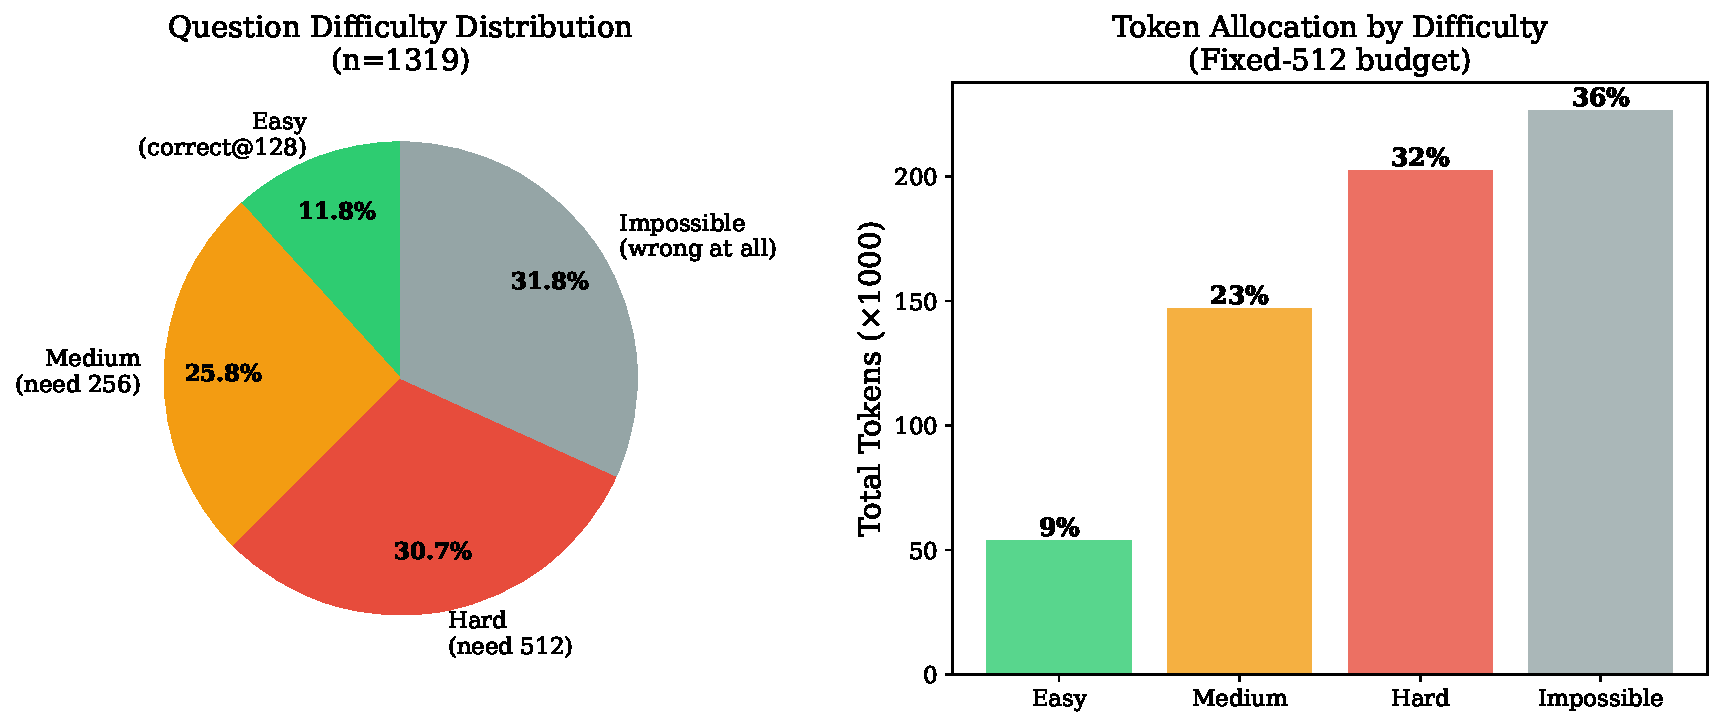
\includegraphics[width=0.72\textwidth]{fig3_difficulty_distribution}
\caption{%
  \textbf{Four-tier difficulty distribution of GSM8K problems} under Qwen3-8B thinking mode.
  Problems are categorized by the minimum budget at which they are solved correctly.
  31.8\% of problems are impossible at all tested budgets---tokens spent on these yield zero return.
  An ideal budget allocator would skip impossible questions and assign minimum budgets to the rest.
}
\label{fig:difficulty-distribution}
\end{figure}

\paragraph{Summary of findings.}
Taken together, our five findings paint a coherent picture:
\begin{enumerate}[nosep,leftmargin=*]
  \item The thinking tax is real and large (\S\ref{sec:finding:tax}):
    non-thinking mode dominates at all matched budgets.
  \item Models already signal when thinking was successful
    (\S\ref{sec:finding:natural-stop}): natural stop predicts 96.3\%
    accuracy at zero cost.
  \item High budgets are under-utilized (\S\ref{sec:finding:utilization}):
    up to 60\% of allocated tokens go unused.
  \item The tax worsens with scale (\S\ref{sec:finding:model-size}):
    larger models need proportionally larger budgets.
  \item A third of problems are impossible
    (\S\ref{sec:finding:impossible}): no budget helps.
\end{enumerate}
The natural question is: can we design a system that \emph{thinks only
when thinking actually helps}?
This is precisely the goal of \textsc{Town}, introduced next.


% ============================================================================
\section{\method{}: \fullmethod{}}
\label{sec:method}
% ============================================================================

% ===========================================================================
%  §4  TOWN: Think Only When Needed
%  method_final.tex — NeurIPS 2026
%  Loaded via % ===========================================================================
%  §4  TOWN: Think Only When Needed
%  method_final.tex — NeurIPS 2026
%  Loaded via % ===========================================================================
%  §4  TOWN: Think Only When Needed
%  method_final.tex — NeurIPS 2026
%  Loaded via \input{sections/method_final}
% ===========================================================================

The empirical findings in \S\ref{sec:thinking-tax} suggest a clear strategy:
\textbf{default to non-thinking mode and reserve thinking for genuinely
hard problems}.
We formalize this intuition as \textsc{Town} (\textbf{T}hink
\textbf{O}nly \textbf{W}hen \textbf{N}eeded), a training-free,
two-stage inference cascade that requires no access to model internals
and no auxiliary models.

% ---------------------------------------------------------------------------
\subsection{Key Insight: Early Stopping as a Difficulty Classifier}
\label{sec:method:insight}
% ---------------------------------------------------------------------------

Our analysis reveals that non-thinking mode's early-stopping behavior
provides a natural binary classifier for problem difficulty:

\begin{observation}
\label{obs:early-stop}
For Qwen3-8B with \texttt{nothink@256} on GSM8K ($n{=}1{,}319$):
\begin{itemize}[nosep,leftmargin=*]
    \item \textbf{88.8\% of samples stop early} (avg 133 tokens),
      achieving \textbf{94.4\%} accuracy among early-stopped samples
      (87.5\% overall).
    \item \textbf{11.2\% of samples hit the budget} (use all 256 tokens),
      indicating the model struggled.
\end{itemize}
\end{observation}

This dichotomy provides a zero-cost routing signal: if the model finishes
quickly in non-thinking mode, the answer is likely correct; if it
exhausts the budget, the problem is likely hard and may benefit from
extended reasoning.
Unlike soft confidence scores or logit-based uncertainty measures, this
signal is \emph{binary}, \emph{endogenous}, and \emph{free}---it emerges
as a byproduct of the generation process itself
(Finding~2, \S\ref{sec:finding:natural-stop}).

% ---------------------------------------------------------------------------
\subsection{The \textsc{Town} Cascade}
\label{sec:method:cascade}
% ---------------------------------------------------------------------------

\textsc{Town} operates in two stages, summarized in
Algorithm~\ref{alg:town} and Figure~\ref{fig:town-pipeline}.

\begin{algorithm}[t]
\caption{\textsc{Town}: Think Only When Needed}
\label{alg:town}
\begin{algorithmic}[1]
\REQUIRE Question $q$, model $\mathcal{M}$,
  probe budget $B_1$ (non-thinking),
  fallback budget $B_2$ (thinking, $B_2 > B_1$)
\ENSURE Answer $\hat{a}$, total tokens consumed $T$

\medskip
\STATE \textbf{// Stage 1: Non-thinking probe}
\STATE $y_1 \leftarrow \mathcal{M}_{\textrm{nt}}(q,\; B_1)$
  \hfill\COMMENT{Generate without thinking}
\STATE $T \leftarrow |y_1|$

\medskip
\IF{$|y_1| < B_1$}
  \hfill\COMMENT{Natural stop $\Rightarrow$ high confidence}
  \STATE $\hat{a} \leftarrow a(y_1)$
  \hfill\COMMENT{Accept non-thinking answer}
\ELSE
  \hfill\COMMENT{Budget hit $\Rightarrow$ low confidence}
  \STATE \textbf{// Stage 2: Thinking fallback}
  \STATE $y_2 \leftarrow \mathcal{M}_{\textrm{th}}(q,\; B_2)$
    \hfill\COMMENT{Generate with chain-of-thought}
  \STATE $T \leftarrow T + |y_2|$
  \STATE $\hat{a} \leftarrow a(y_2)$
  \hfill\COMMENT{Use thinking answer}
\ENDIF

\medskip
\RETURN $\hat{a},\; T$
\end{algorithmic}
\end{algorithm}

\input{sections/fig_town_pipeline}

\paragraph{Stage 1: Non-thinking probe.}
We run the input through non-thinking mode with a moderate budget
$B_1$ (default: 256 tokens).
If the model produces a complete answer before exhausting $B_1$, we
accept it immediately.
This stage handles the vast majority of inputs---88.8\% on GSM8K---at
minimal cost (${\sim}$133 tokens on average for early-stopped samples), exploiting Finding~1's
observation that non-thinking mode is more token-efficient than thinking
mode at matched budgets.

\paragraph{Stage 2: Thinking fallback.}
For the ${\sim}$11.2\% of inputs that exhaust the Stage~1 budget---indicating
the model could not produce a confident answer quickly---we route to
thinking mode with an extended budget $B_2$ (default: 512 tokens).
These are precisely the ``hard'' problems where step-by-step reasoning
chains are most likely to provide genuine benefit.
The total cost for a fallback sample is $B_1 + |y_2|$, since the
probe consumed its full budget.

% ---------------------------------------------------------------------------
\subsection{Cost and Accuracy Analysis}
\label{sec:method:analysis}
% ---------------------------------------------------------------------------

\paragraph{Expected token cost.}
Let $p$ denote the early-stop rate in Stage~1,
$\bar{t}_1$ the average tokens for early-stopped samples, and
$\bar{t}_2$ the average thinking-mode cost for fallback samples.
The expected token cost per question is:
\begin{equation}
  \label{eq:town-cost}
  \mathbb{E}[T] \;=\; p \cdot \bar{t}_1
    \;+\; (1 - p) \cdot \big(B_1 + \bar{t}_2\big).
\end{equation}
With our GSM8K parameters ($p{=}0.888$, $\bar{t}_1{\approx}133$,
$B_1{=}256$, $\bar{t}_2{\approx}469$) on the full test set ($n{=}1{,}319$):
\begin{equation}
  \label{eq:town-cost-concrete}
  \mathbb{E}[T]
    \;\approx\; 0.888 \times 133 \;+\; 0.112 \times (256 + 469)
    \;\approx\; 118 + 81
    \;=\; \mathbf{\sim\!199\text{ tokens}}.
\end{equation}
This is \textbf{2.4$\times$} cheaper than \texttt{think@512} alone
(460~tokens), representing a \textbf{57\%} reduction in average token
consumption.  Note that the Stage~1 probe budget $B_1$ is ``spent''
even for routed samples---it serves as the cost of difficulty
classification.

\paragraph{Projected accuracy.}
\textsc{Town}'s accuracy decomposes as:
\begin{equation}
  \label{eq:town-acc}
  \textrm{Acc}_{\textsc{Town}}
    \;=\; p \cdot \textrm{Acc}_{\textrm{nt}}^{\textrm{early}}
    \;+\; (1 - p) \cdot \textrm{Acc}_{\textrm{th}}^{\textrm{hard}},
\end{equation}
where $\textrm{Acc}_{\textrm{nt}}^{\textrm{early}}$ is the
accuracy of early-stop non-thinking samples and
$\textrm{Acc}_{\textrm{th}}^{\textrm{hard}}$ is the thinking-mode
accuracy on the hard subset routed to Stage~2.
On the full GSM8K test set ($n{=}1{,}319$),
\textsc{Town} achieves \textbf{90.9\%} accuracy at only \textbf{199
average tokens} (including the Stage~1 probe cost for routed samples):
\begin{equation}
  \textrm{Acc}_{\textsc{Town}}
    \;=\; \underbrace{0.888 \times 94.4\%}_{\text{Stage 1: early-stop}}
    \;+\; \underbrace{0.112 \times 62.8\%}_{\text{Stage 2: thinking fallback}}
    \;=\; 83.8\% + 7.0\%
    \;=\; \mathbf{90.9\%}.
\end{equation}
This exceeds \texttt{think@512} (65.2\%) by \textbf{+25.7\,pp}
while using \textbf{2.4$\times$ fewer tokens}, and surpasses
\texttt{nothink@256} (87.5\%) by \textbf{+3.4\,pp} by recovering
hard cases through Stage~2.
Full evaluation results are in \S\ref{sec:town-eval}.

% ---------------------------------------------------------------------------
\subsection{Comparison with Alternative Strategies}
\label{sec:method:comparison}
% ---------------------------------------------------------------------------

\paragraph{vs.\ \texttt{think@512} only.}
\textsc{Town} achieves substantially higher accuracy at
${\sim}$2.4$\times$ fewer tokens.
The advantage comes from avoiding thinking mode's truncation waste on the
88.8\% of problems where it is unnecessary.

\paragraph{vs.\ \texttt{nothink@256} only.}
\textsc{Town} adds a thinking fallback for the $\sim$11.2\% of hard
problems, recovering accuracy on cases where direct answering
fails.
The additional cost is modest: $\sim$53 extra tokens on average
over the entire dataset (199 vs.\ 146 for \texttt{nothink@256}).

\paragraph{vs.\ Self-consistency~\cite{wang2023selfconsistency}.}
SC@$K$ generates $K$ full-budget reasoning traces and majority-votes,
consuming $K \times B$ tokens unconditionally.
\textsc{Town} uses a \emph{single} non-thinking probe and a binary
routing decision, yielding lower latency (one generation call for easy
questions vs.\ $K$), lower token cost ($\sim$146 tokens for easy
questions vs.\ $K \times B$), and a simpler implementation (no consensus
computation, no threshold tuning).

\paragraph{vs.\ Oracle routing.}
An oracle that knows each problem's difficulty \emph{a priori}
achieves 68.2\% accuracy at 401 average tokens
(Table~\ref{tab:efficiency-frontier}).
\textsc{Town}'s early-stop signal approximates this oracle using a
training-free heuristic, with the gap determined primarily by the
signal's precision on the routed subset.

\paragraph{Hyperparameters.}
\textsc{Town} introduces exactly \emph{two} hyperparameters beyond the
base model: $B_1$ (probe budget) and $B_2$ (thinking fallback budget).
Both have intuitive interpretations: $B_1$ should be large enough for
the model to produce a complete non-thinking answer on most easy
questions (256 tokens suffices for GSM8K), and $B_2$ should be large
enough for a complete reasoning chain on hard questions (512+ for
GSM8K).
No routing thresholds, consensus weights, or learned parameters are
required.

% ===========================================================================

The empirical findings in \S\ref{sec:thinking-tax} suggest a clear strategy:
\textbf{default to non-thinking mode and reserve thinking for genuinely
hard problems}.
We formalize this intuition as \textsc{Town} (\textbf{T}hink
\textbf{O}nly \textbf{W}hen \textbf{N}eeded), a training-free,
two-stage inference cascade that requires no access to model internals
and no auxiliary models.

% ---------------------------------------------------------------------------
\subsection{Key Insight: Early Stopping as a Difficulty Classifier}
\label{sec:method:insight}
% ---------------------------------------------------------------------------

Our analysis reveals that non-thinking mode's early-stopping behavior
provides a natural binary classifier for problem difficulty:

\begin{observation}
\label{obs:early-stop}
For Qwen3-8B with \texttt{nothink@256} on GSM8K ($n{=}1{,}319$):
\begin{itemize}[nosep,leftmargin=*]
    \item \textbf{88.8\% of samples stop early} (avg 133 tokens),
      achieving \textbf{94.4\%} accuracy among early-stopped samples
      (87.5\% overall).
    \item \textbf{11.2\% of samples hit the budget} (use all 256 tokens),
      indicating the model struggled.
\end{itemize}
\end{observation}

This dichotomy provides a zero-cost routing signal: if the model finishes
quickly in non-thinking mode, the answer is likely correct; if it
exhausts the budget, the problem is likely hard and may benefit from
extended reasoning.
Unlike soft confidence scores or logit-based uncertainty measures, this
signal is \emph{binary}, \emph{endogenous}, and \emph{free}---it emerges
as a byproduct of the generation process itself
(Finding~2, \S\ref{sec:finding:natural-stop}).

% ---------------------------------------------------------------------------
\subsection{The \textsc{Town} Cascade}
\label{sec:method:cascade}
% ---------------------------------------------------------------------------

\textsc{Town} operates in two stages, summarized in
Algorithm~\ref{alg:town} and Figure~\ref{fig:town-pipeline}.

\begin{algorithm}[t]
\caption{\textsc{Town}: Think Only When Needed}
\label{alg:town}
\begin{algorithmic}[1]
\REQUIRE Question $q$, model $\mathcal{M}$,
  probe budget $B_1$ (non-thinking),
  fallback budget $B_2$ (thinking, $B_2 > B_1$)
\ENSURE Answer $\hat{a}$, total tokens consumed $T$

\medskip
\STATE \textbf{// Stage 1: Non-thinking probe}
\STATE $y_1 \leftarrow \mathcal{M}_{\textrm{nt}}(q,\; B_1)$
  \hfill\COMMENT{Generate without thinking}
\STATE $T \leftarrow |y_1|$

\medskip
\IF{$|y_1| < B_1$}
  \hfill\COMMENT{Natural stop $\Rightarrow$ high confidence}
  \STATE $\hat{a} \leftarrow a(y_1)$
  \hfill\COMMENT{Accept non-thinking answer}
\ELSE
  \hfill\COMMENT{Budget hit $\Rightarrow$ low confidence}
  \STATE \textbf{// Stage 2: Thinking fallback}
  \STATE $y_2 \leftarrow \mathcal{M}_{\textrm{th}}(q,\; B_2)$
    \hfill\COMMENT{Generate with chain-of-thought}
  \STATE $T \leftarrow T + |y_2|$
  \STATE $\hat{a} \leftarrow a(y_2)$
  \hfill\COMMENT{Use thinking answer}
\ENDIF

\medskip
\RETURN $\hat{a},\; T$
\end{algorithmic}
\end{algorithm}

% fig_town_pipeline.tex — TikZ pipeline diagram for TOWN method
% Include in method_final.tex via \input{sections/fig_town_pipeline}

\begin{figure}[t]
\centering
\resizebox{\linewidth}{!}{%
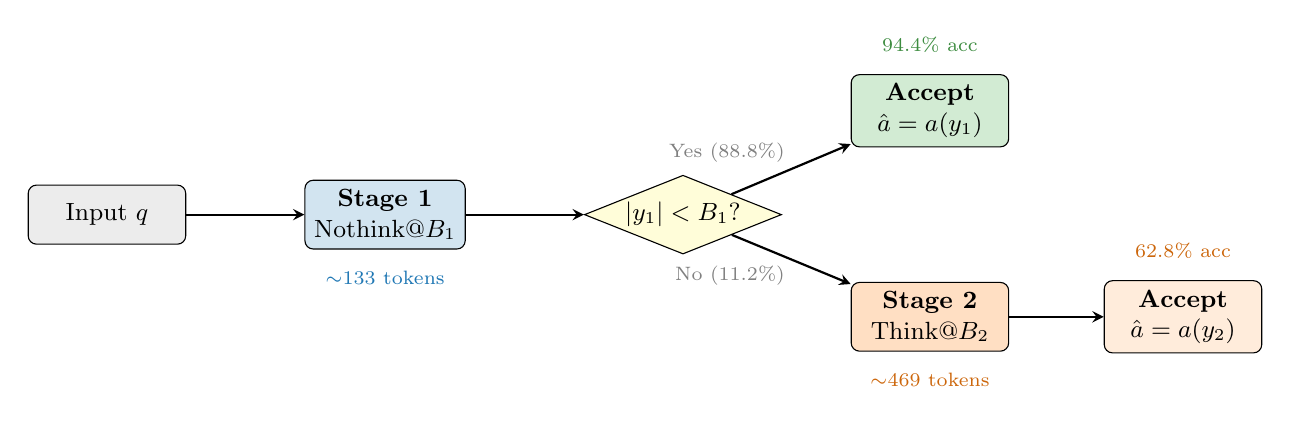
\begin{tikzpicture}[
    node distance=1.0cm and 1.2cm,
    box/.style={rectangle, draw, rounded corners=3pt, minimum width=2.0cm,
                minimum height=0.75cm, align=center, font=\small},
    decision/.style={diamond, draw, aspect=2.5, inner sep=1pt,
                     align=center, font=\small},
    arrow/.style={->, thick, >=stealth},
    label/.style={font=\scriptsize, text=gray},
]

% Input
\node[box, fill=gray!15] (input) {Input $q$};

% Stage 1
\node[box, fill=nothinkblue!20, right=1.5cm of input] (s1)
    {\textbf{Stage 1}\\Nothink@$B_1$};

% Decision
\node[decision, fill=yellow!15, right=1.5cm of s1] (dec)
    {$|y_1|<B_1$?};

% Accept
\node[box, fill=easycolor!25, above right=0.6cm and 1.5cm of dec] (accept)
    {\textbf{Accept}\\$\hat{a}=a(y_1)$};

% Stage 2
\node[box, fill=thinkorange!25, below right=0.6cm and 1.5cm of dec] (s2)
    {\textbf{Stage 2}\\Think@$B_2$};

% Final
\node[box, fill=thinkorange!15, right=1.2cm of s2] (final2)
    {\textbf{Accept}\\$\hat{a}=a(y_2)$};

% Arrows
\draw[arrow] (input) -- (s1);
\draw[arrow] (s1) -- (dec);
\draw[arrow] (dec) -- node[label, above left=-2pt] {Yes (88.8\%)} (accept);
\draw[arrow] (dec) -- node[label, below left=-2pt] {No (11.2\%)} (s2);
\draw[arrow] (s2) -- (final2);

% Annotations
\node[below=0.15cm of s1, font=\scriptsize, text=nothinkblue]
    {$\sim$133 tokens};
\node[above=0.15cm of accept, font=\scriptsize, text=easycolor!80!black]
    {94.4\% acc};
\node[below=0.15cm of s2, font=\scriptsize, text=thinkorange!80!black]
    {$\sim$469 tokens};
\node[above=0.15cm of final2, font=\scriptsize, text=thinkorange!80!black]
    {62.8\% acc};

\end{tikzpicture}%
}
\caption{%
    \textbf{\town{} baseline inference pipeline.}
    Stage~1 probes with non-thinking mode at budget $B_1$.
    If the model stops early (88.8\% of GSM8K), the answer is accepted
    at ${\sim}$133 tokens (94.4\% accuracy).
    Otherwise, Stage~2 routes to thinking mode at budget $B_2$,
    recovering additional correct answers on hard problems.
    Overall: \textbf{90.9\%} accuracy at \textbf{199} average tokens on the full test set ($n{=}1{,}319$).
    Note: \method{} extends this with decoupled answer generation and iterative refinement (Algorithm~\ref{alg:mrsd}).
}
\label{fig:town-pipeline}
\end{figure}


\paragraph{Stage 1: Non-thinking probe.}
We run the input through non-thinking mode with a moderate budget
$B_1$ (default: 256 tokens).
If the model produces a complete answer before exhausting $B_1$, we
accept it immediately.
This stage handles the vast majority of inputs---88.8\% on GSM8K---at
minimal cost (${\sim}$133 tokens on average for early-stopped samples), exploiting Finding~1's
observation that non-thinking mode is more token-efficient than thinking
mode at matched budgets.

\paragraph{Stage 2: Thinking fallback.}
For the ${\sim}$11.2\% of inputs that exhaust the Stage~1 budget---indicating
the model could not produce a confident answer quickly---we route to
thinking mode with an extended budget $B_2$ (default: 512 tokens).
These are precisely the ``hard'' problems where step-by-step reasoning
chains are most likely to provide genuine benefit.
The total cost for a fallback sample is $B_1 + |y_2|$, since the
probe consumed its full budget.

% ---------------------------------------------------------------------------
\subsection{Cost and Accuracy Analysis}
\label{sec:method:analysis}
% ---------------------------------------------------------------------------

\paragraph{Expected token cost.}
Let $p$ denote the early-stop rate in Stage~1,
$\bar{t}_1$ the average tokens for early-stopped samples, and
$\bar{t}_2$ the average thinking-mode cost for fallback samples.
The expected token cost per question is:
\begin{equation}
  \label{eq:town-cost}
  \mathbb{E}[T] \;=\; p \cdot \bar{t}_1
    \;+\; (1 - p) \cdot \big(B_1 + \bar{t}_2\big).
\end{equation}
With our GSM8K parameters ($p{=}0.888$, $\bar{t}_1{\approx}133$,
$B_1{=}256$, $\bar{t}_2{\approx}469$) on the full test set ($n{=}1{,}319$):
\begin{equation}
  \label{eq:town-cost-concrete}
  \mathbb{E}[T]
    \;\approx\; 0.888 \times 133 \;+\; 0.112 \times (256 + 469)
    \;\approx\; 118 + 81
    \;=\; \mathbf{\sim\!199\text{ tokens}}.
\end{equation}
This is \textbf{2.4$\times$} cheaper than \texttt{think@512} alone
(460~tokens), representing a \textbf{57\%} reduction in average token
consumption.  Note that the Stage~1 probe budget $B_1$ is ``spent''
even for routed samples---it serves as the cost of difficulty
classification.

\paragraph{Projected accuracy.}
\textsc{Town}'s accuracy decomposes as:
\begin{equation}
  \label{eq:town-acc}
  \textrm{Acc}_{\textsc{Town}}
    \;=\; p \cdot \textrm{Acc}_{\textrm{nt}}^{\textrm{early}}
    \;+\; (1 - p) \cdot \textrm{Acc}_{\textrm{th}}^{\textrm{hard}},
\end{equation}
where $\textrm{Acc}_{\textrm{nt}}^{\textrm{early}}$ is the
accuracy of early-stop non-thinking samples and
$\textrm{Acc}_{\textrm{th}}^{\textrm{hard}}$ is the thinking-mode
accuracy on the hard subset routed to Stage~2.
On the full GSM8K test set ($n{=}1{,}319$),
\textsc{Town} achieves \textbf{90.9\%} accuracy at only \textbf{199
average tokens} (including the Stage~1 probe cost for routed samples):
\begin{equation}
  \textrm{Acc}_{\textsc{Town}}
    \;=\; \underbrace{0.888 \times 94.4\%}_{\text{Stage 1: early-stop}}
    \;+\; \underbrace{0.112 \times 62.8\%}_{\text{Stage 2: thinking fallback}}
    \;=\; 83.8\% + 7.0\%
    \;=\; \mathbf{90.9\%}.
\end{equation}
This exceeds \texttt{think@512} (65.2\%) by \textbf{+25.7\,pp}
while using \textbf{2.4$\times$ fewer tokens}, and surpasses
\texttt{nothink@256} (87.5\%) by \textbf{+3.4\,pp} by recovering
hard cases through Stage~2.
Full evaluation results are in \S\ref{sec:town-eval}.

% ---------------------------------------------------------------------------
\subsection{Comparison with Alternative Strategies}
\label{sec:method:comparison}
% ---------------------------------------------------------------------------

\paragraph{vs.\ \texttt{think@512} only.}
\textsc{Town} achieves substantially higher accuracy at
${\sim}$2.4$\times$ fewer tokens.
The advantage comes from avoiding thinking mode's truncation waste on the
88.8\% of problems where it is unnecessary.

\paragraph{vs.\ \texttt{nothink@256} only.}
\textsc{Town} adds a thinking fallback for the $\sim$11.2\% of hard
problems, recovering accuracy on cases where direct answering
fails.
The additional cost is modest: $\sim$53 extra tokens on average
over the entire dataset (199 vs.\ 146 for \texttt{nothink@256}).

\paragraph{vs.\ Self-consistency~\cite{wang2023selfconsistency}.}
SC@$K$ generates $K$ full-budget reasoning traces and majority-votes,
consuming $K \times B$ tokens unconditionally.
\textsc{Town} uses a \emph{single} non-thinking probe and a binary
routing decision, yielding lower latency (one generation call for easy
questions vs.\ $K$), lower token cost ($\sim$146 tokens for easy
questions vs.\ $K \times B$), and a simpler implementation (no consensus
computation, no threshold tuning).

\paragraph{vs.\ Oracle routing.}
An oracle that knows each problem's difficulty \emph{a priori}
achieves 68.2\% accuracy at 401 average tokens
(Table~\ref{tab:efficiency-frontier}).
\textsc{Town}'s early-stop signal approximates this oracle using a
training-free heuristic, with the gap determined primarily by the
signal's precision on the routed subset.

\paragraph{Hyperparameters.}
\textsc{Town} introduces exactly \emph{two} hyperparameters beyond the
base model: $B_1$ (probe budget) and $B_2$ (thinking fallback budget).
Both have intuitive interpretations: $B_1$ should be large enough for
the model to produce a complete non-thinking answer on most easy
questions (256 tokens suffices for GSM8K), and $B_2$ should be large
enough for a complete reasoning chain on hard questions (512+ for
GSM8K).
No routing thresholds, consensus weights, or learned parameters are
required.

% ===========================================================================

The empirical findings in \S\ref{sec:thinking-tax} suggest a clear strategy:
\textbf{default to non-thinking mode and reserve thinking for genuinely
hard problems}.
We formalize this intuition as \textsc{Town} (\textbf{T}hink
\textbf{O}nly \textbf{W}hen \textbf{N}eeded), a training-free,
two-stage inference cascade that requires no access to model internals
and no auxiliary models.

% ---------------------------------------------------------------------------
\subsection{Key Insight: Early Stopping as a Difficulty Classifier}
\label{sec:method:insight}
% ---------------------------------------------------------------------------

Our analysis reveals that non-thinking mode's early-stopping behavior
provides a natural binary classifier for problem difficulty:

\begin{observation}
\label{obs:early-stop}
For Qwen3-8B with \texttt{nothink@256} on GSM8K ($n{=}1{,}319$):
\begin{itemize}[nosep,leftmargin=*]
    \item \textbf{88.8\% of samples stop early} (avg 133 tokens),
      achieving \textbf{94.4\%} accuracy among early-stopped samples
      (87.5\% overall).
    \item \textbf{11.2\% of samples hit the budget} (use all 256 tokens),
      indicating the model struggled.
\end{itemize}
\end{observation}

This dichotomy provides a zero-cost routing signal: if the model finishes
quickly in non-thinking mode, the answer is likely correct; if it
exhausts the budget, the problem is likely hard and may benefit from
extended reasoning.
Unlike soft confidence scores or logit-based uncertainty measures, this
signal is \emph{binary}, \emph{endogenous}, and \emph{free}---it emerges
as a byproduct of the generation process itself
(Finding~2, \S\ref{sec:finding:natural-stop}).

% ---------------------------------------------------------------------------
\subsection{The \textsc{Town} Cascade}
\label{sec:method:cascade}
% ---------------------------------------------------------------------------

\textsc{Town} operates in two stages, summarized in
Algorithm~\ref{alg:town} and Figure~\ref{fig:town-pipeline}.

\begin{algorithm}[t]
\caption{\textsc{Town}: Think Only When Needed}
\label{alg:town}
\begin{algorithmic}[1]
\REQUIRE Question $q$, model $\mathcal{M}$,
  probe budget $B_1$ (non-thinking),
  fallback budget $B_2$ (thinking, $B_2 > B_1$)
\ENSURE Answer $\hat{a}$, total tokens consumed $T$

\medskip
\STATE \textbf{// Stage 1: Non-thinking probe}
\STATE $y_1 \leftarrow \mathcal{M}_{\textrm{nt}}(q,\; B_1)$
  \hfill\COMMENT{Generate without thinking}
\STATE $T \leftarrow |y_1|$

\medskip
\IF{$|y_1| < B_1$}
  \hfill\COMMENT{Natural stop $\Rightarrow$ high confidence}
  \STATE $\hat{a} \leftarrow a(y_1)$
  \hfill\COMMENT{Accept non-thinking answer}
\ELSE
  \hfill\COMMENT{Budget hit $\Rightarrow$ low confidence}
  \STATE \textbf{// Stage 2: Thinking fallback}
  \STATE $y_2 \leftarrow \mathcal{M}_{\textrm{th}}(q,\; B_2)$
    \hfill\COMMENT{Generate with chain-of-thought}
  \STATE $T \leftarrow T + |y_2|$
  \STATE $\hat{a} \leftarrow a(y_2)$
  \hfill\COMMENT{Use thinking answer}
\ENDIF

\medskip
\RETURN $\hat{a},\; T$
\end{algorithmic}
\end{algorithm}

% fig_town_pipeline.tex — TikZ pipeline diagram for TOWN method
% Include in method_final.tex via % fig_town_pipeline.tex — TikZ pipeline diagram for TOWN method
% Include in method_final.tex via \input{sections/fig_town_pipeline}

\begin{figure}[t]
\centering
\resizebox{\linewidth}{!}{%
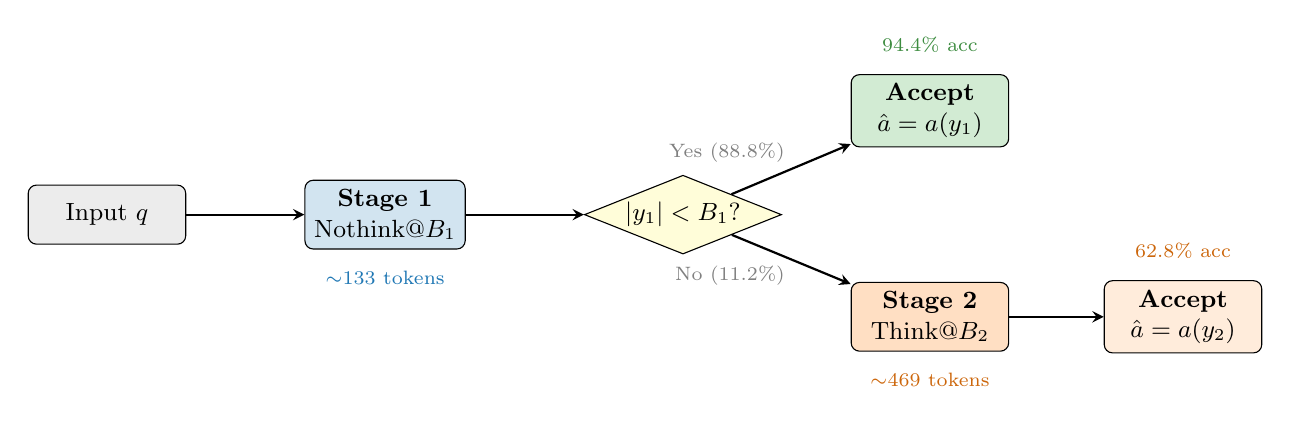
\begin{tikzpicture}[
    node distance=1.0cm and 1.2cm,
    box/.style={rectangle, draw, rounded corners=3pt, minimum width=2.0cm,
                minimum height=0.75cm, align=center, font=\small},
    decision/.style={diamond, draw, aspect=2.5, inner sep=1pt,
                     align=center, font=\small},
    arrow/.style={->, thick, >=stealth},
    label/.style={font=\scriptsize, text=gray},
]

% Input
\node[box, fill=gray!15] (input) {Input $q$};

% Stage 1
\node[box, fill=nothinkblue!20, right=1.5cm of input] (s1)
    {\textbf{Stage 1}\\Nothink@$B_1$};

% Decision
\node[decision, fill=yellow!15, right=1.5cm of s1] (dec)
    {$|y_1|<B_1$?};

% Accept
\node[box, fill=easycolor!25, above right=0.6cm and 1.5cm of dec] (accept)
    {\textbf{Accept}\\$\hat{a}=a(y_1)$};

% Stage 2
\node[box, fill=thinkorange!25, below right=0.6cm and 1.5cm of dec] (s2)
    {\textbf{Stage 2}\\Think@$B_2$};

% Final
\node[box, fill=thinkorange!15, right=1.2cm of s2] (final2)
    {\textbf{Accept}\\$\hat{a}=a(y_2)$};

% Arrows
\draw[arrow] (input) -- (s1);
\draw[arrow] (s1) -- (dec);
\draw[arrow] (dec) -- node[label, above left=-2pt] {Yes (88.8\%)} (accept);
\draw[arrow] (dec) -- node[label, below left=-2pt] {No (11.2\%)} (s2);
\draw[arrow] (s2) -- (final2);

% Annotations
\node[below=0.15cm of s1, font=\scriptsize, text=nothinkblue]
    {$\sim$133 tokens};
\node[above=0.15cm of accept, font=\scriptsize, text=easycolor!80!black]
    {94.4\% acc};
\node[below=0.15cm of s2, font=\scriptsize, text=thinkorange!80!black]
    {$\sim$469 tokens};
\node[above=0.15cm of final2, font=\scriptsize, text=thinkorange!80!black]
    {62.8\% acc};

\end{tikzpicture}%
}
\caption{%
    \textbf{\town{} baseline inference pipeline.}
    Stage~1 probes with non-thinking mode at budget $B_1$.
    If the model stops early (88.8\% of GSM8K), the answer is accepted
    at ${\sim}$133 tokens (94.4\% accuracy).
    Otherwise, Stage~2 routes to thinking mode at budget $B_2$,
    recovering additional correct answers on hard problems.
    Overall: \textbf{90.9\%} accuracy at \textbf{199} average tokens on the full test set ($n{=}1{,}319$).
    Note: \method{} extends this with decoupled answer generation and iterative refinement (Algorithm~\ref{alg:mrsd}).
}
\label{fig:town-pipeline}
\end{figure}


\begin{figure}[t]
\centering
\resizebox{\linewidth}{!}{%
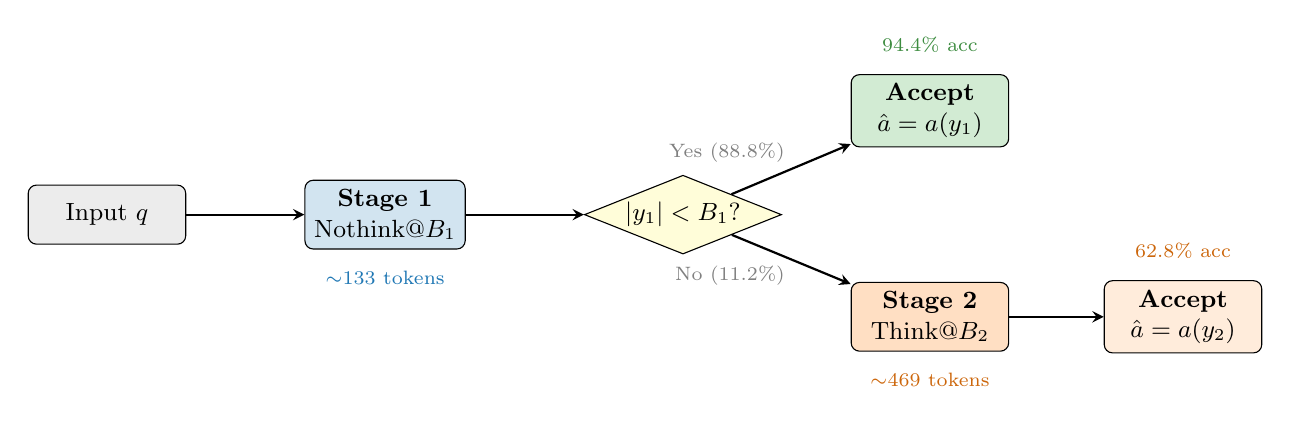
\begin{tikzpicture}[
    node distance=1.0cm and 1.2cm,
    box/.style={rectangle, draw, rounded corners=3pt, minimum width=2.0cm,
                minimum height=0.75cm, align=center, font=\small},
    decision/.style={diamond, draw, aspect=2.5, inner sep=1pt,
                     align=center, font=\small},
    arrow/.style={->, thick, >=stealth},
    label/.style={font=\scriptsize, text=gray},
]

% Input
\node[box, fill=gray!15] (input) {Input $q$};

% Stage 1
\node[box, fill=nothinkblue!20, right=1.5cm of input] (s1)
    {\textbf{Stage 1}\\Nothink@$B_1$};

% Decision
\node[decision, fill=yellow!15, right=1.5cm of s1] (dec)
    {$|y_1|<B_1$?};

% Accept
\node[box, fill=easycolor!25, above right=0.6cm and 1.5cm of dec] (accept)
    {\textbf{Accept}\\$\hat{a}=a(y_1)$};

% Stage 2
\node[box, fill=thinkorange!25, below right=0.6cm and 1.5cm of dec] (s2)
    {\textbf{Stage 2}\\Think@$B_2$};

% Final
\node[box, fill=thinkorange!15, right=1.2cm of s2] (final2)
    {\textbf{Accept}\\$\hat{a}=a(y_2)$};

% Arrows
\draw[arrow] (input) -- (s1);
\draw[arrow] (s1) -- (dec);
\draw[arrow] (dec) -- node[label, above left=-2pt] {Yes (88.8\%)} (accept);
\draw[arrow] (dec) -- node[label, below left=-2pt] {No (11.2\%)} (s2);
\draw[arrow] (s2) -- (final2);

% Annotations
\node[below=0.15cm of s1, font=\scriptsize, text=nothinkblue]
    {$\sim$133 tokens};
\node[above=0.15cm of accept, font=\scriptsize, text=easycolor!80!black]
    {94.4\% acc};
\node[below=0.15cm of s2, font=\scriptsize, text=thinkorange!80!black]
    {$\sim$469 tokens};
\node[above=0.15cm of final2, font=\scriptsize, text=thinkorange!80!black]
    {62.8\% acc};

\end{tikzpicture}%
}
\caption{%
    \textbf{\town{} baseline inference pipeline.}
    Stage~1 probes with non-thinking mode at budget $B_1$.
    If the model stops early (88.8\% of GSM8K), the answer is accepted
    at ${\sim}$133 tokens (94.4\% accuracy).
    Otherwise, Stage~2 routes to thinking mode at budget $B_2$,
    recovering additional correct answers on hard problems.
    Overall: \textbf{90.9\%} accuracy at \textbf{199} average tokens on the full test set ($n{=}1{,}319$).
    Note: \method{} extends this with decoupled answer generation and iterative refinement (Algorithm~\ref{alg:mrsd}).
}
\label{fig:town-pipeline}
\end{figure}


\paragraph{Stage 1: Non-thinking probe.}
We run the input through non-thinking mode with a moderate budget
$B_1$ (default: 256 tokens).
If the model produces a complete answer before exhausting $B_1$, we
accept it immediately.
This stage handles the vast majority of inputs---88.8\% on GSM8K---at
minimal cost (${\sim}$133 tokens on average for early-stopped samples), exploiting Finding~1's
observation that non-thinking mode is more token-efficient than thinking
mode at matched budgets.

\paragraph{Stage 2: Thinking fallback.}
For the ${\sim}$11.2\% of inputs that exhaust the Stage~1 budget---indicating
the model could not produce a confident answer quickly---we route to
thinking mode with an extended budget $B_2$ (default: 512 tokens).
These are precisely the ``hard'' problems where step-by-step reasoning
chains are most likely to provide genuine benefit.
The total cost for a fallback sample is $B_1 + |y_2|$, since the
probe consumed its full budget.

% ---------------------------------------------------------------------------
\subsection{Cost and Accuracy Analysis}
\label{sec:method:analysis}
% ---------------------------------------------------------------------------

\paragraph{Expected token cost.}
Let $p$ denote the early-stop rate in Stage~1,
$\bar{t}_1$ the average tokens for early-stopped samples, and
$\bar{t}_2$ the average thinking-mode cost for fallback samples.
The expected token cost per question is:
\begin{equation}
  \label{eq:town-cost}
  \mathbb{E}[T] \;=\; p \cdot \bar{t}_1
    \;+\; (1 - p) \cdot \big(B_1 + \bar{t}_2\big).
\end{equation}
With our GSM8K parameters ($p{=}0.888$, $\bar{t}_1{\approx}133$,
$B_1{=}256$, $\bar{t}_2{\approx}469$) on the full test set ($n{=}1{,}319$):
\begin{equation}
  \label{eq:town-cost-concrete}
  \mathbb{E}[T]
    \;\approx\; 0.888 \times 133 \;+\; 0.112 \times (256 + 469)
    \;\approx\; 118 + 81
    \;=\; \mathbf{\sim\!199\text{ tokens}}.
\end{equation}
This is \textbf{2.4$\times$} cheaper than \texttt{think@512} alone
(460~tokens), representing a \textbf{57\%} reduction in average token
consumption.  Note that the Stage~1 probe budget $B_1$ is ``spent''
even for routed samples---it serves as the cost of difficulty
classification.

\paragraph{Projected accuracy.}
\textsc{Town}'s accuracy decomposes as:
\begin{equation}
  \label{eq:town-acc}
  \textrm{Acc}_{\textsc{Town}}
    \;=\; p \cdot \textrm{Acc}_{\textrm{nt}}^{\textrm{early}}
    \;+\; (1 - p) \cdot \textrm{Acc}_{\textrm{th}}^{\textrm{hard}},
\end{equation}
where $\textrm{Acc}_{\textrm{nt}}^{\textrm{early}}$ is the
accuracy of early-stop non-thinking samples and
$\textrm{Acc}_{\textrm{th}}^{\textrm{hard}}$ is the thinking-mode
accuracy on the hard subset routed to Stage~2.
On the full GSM8K test set ($n{=}1{,}319$),
\textsc{Town} achieves \textbf{90.9\%} accuracy at only \textbf{199
average tokens} (including the Stage~1 probe cost for routed samples):
\begin{equation}
  \textrm{Acc}_{\textsc{Town}}
    \;=\; \underbrace{0.888 \times 94.4\%}_{\text{Stage 1: early-stop}}
    \;+\; \underbrace{0.112 \times 62.8\%}_{\text{Stage 2: thinking fallback}}
    \;=\; 83.8\% + 7.0\%
    \;=\; \mathbf{90.9\%}.
\end{equation}
This exceeds \texttt{think@512} (65.2\%) by \textbf{+25.7\,pp}
while using \textbf{2.4$\times$ fewer tokens}, and surpasses
\texttt{nothink@256} (87.5\%) by \textbf{+3.4\,pp} by recovering
hard cases through Stage~2.
Full evaluation results are in \S\ref{sec:town-eval}.

% ---------------------------------------------------------------------------
\subsection{Comparison with Alternative Strategies}
\label{sec:method:comparison}
% ---------------------------------------------------------------------------

\paragraph{vs.\ \texttt{think@512} only.}
\textsc{Town} achieves substantially higher accuracy at
${\sim}$2.4$\times$ fewer tokens.
The advantage comes from avoiding thinking mode's truncation waste on the
88.8\% of problems where it is unnecessary.

\paragraph{vs.\ \texttt{nothink@256} only.}
\textsc{Town} adds a thinking fallback for the $\sim$11.2\% of hard
problems, recovering accuracy on cases where direct answering
fails.
The additional cost is modest: $\sim$53 extra tokens on average
over the entire dataset (199 vs.\ 146 for \texttt{nothink@256}).

\paragraph{vs.\ Self-consistency~\cite{wang2023selfconsistency}.}
SC@$K$ generates $K$ full-budget reasoning traces and majority-votes,
consuming $K \times B$ tokens unconditionally.
\textsc{Town} uses a \emph{single} non-thinking probe and a binary
routing decision, yielding lower latency (one generation call for easy
questions vs.\ $K$), lower token cost ($\sim$146 tokens for easy
questions vs.\ $K \times B$), and a simpler implementation (no consensus
computation, no threshold tuning).

\paragraph{vs.\ Oracle routing.}
An oracle that knows each problem's difficulty \emph{a priori}
achieves 68.2\% accuracy at 401 average tokens
(Table~\ref{tab:efficiency-frontier}).
\textsc{Town}'s early-stop signal approximates this oracle using a
training-free heuristic, with the gap determined primarily by the
signal's precision on the routed subset.

\paragraph{Hyperparameters.}
\textsc{Town} introduces exactly \emph{two} hyperparameters beyond the
base model: $B_1$ (probe budget) and $B_2$ (thinking fallback budget).
Both have intuitive interpretations: $B_1$ should be large enough for
the model to produce a complete non-thinking answer on most easy
questions (256 tokens suffices for GSM8K), and $B_2$ should be large
enough for a complete reasoning chain on hard questions (512+ for
GSM8K).
No routing thresholds, consensus weights, or learned parameters are
required.


% ============================================================================
\section{Experiments}
\label{sec:experiments}
% ============================================================================

% experiments_final.tex — §5 Experiments: TOWN evaluation and cross-model validation
% Empirical findings (§3) already cover the thinking tax analysis.
% This section focuses on (1) evaluating TOWN and (2) cross-model generalization.

\subsection{\method{} Evaluation on GSM8K}
\label{sec:town-eval}

We evaluate \method{} (Algorithm~\ref{alg:town}) with $B_1{=}256$ (non-thinking) and $B_2{=}512$ (thinking) on the \textbf{full GSM8K test set} ($n{=}1{,}319$) using Qwen3-8B, where we have matched per-sample results for both modes.

\paragraph{Stage 1: Non-thinking probe.}
Running \texttt{nothink@256}, 88.8\% of samples (1{,}171/1{,}319) stop early with 94.4\% accuracy among early-stopped samples.
The average token consumption for early-stopped samples is only ${\sim}$133 tokens.
The remaining 11.2\% (148 samples) exhaust the 256-token budget, triggering Stage~2.

\paragraph{Stage 2: Thinking fallback.}
The 148 routed samples receive \texttt{think@512}.
These are precisely the ``hard'' problems where non-thinking mode could not produce a confident answer within the probe budget.
Among this subset, thinking mode achieves 62.8\% accuracy (93/148)---recovering correct answers on the majority of hard cases where direct answering failed.

\paragraph{End-to-end results.}
Table~\ref{tab:town-comparison} compares \method{} against single-mode baselines.
\method{} achieves \textbf{90.9\%} accuracy at only \textbf{199 average tokens}
(including the Stage~1 probe cost for all samples)---the best of both worlds.

\begin{table}[t]
\centering
\caption{\textbf{\method{} vs.\ single-mode baselines} on the full GSM8K test set ($n{=}1{,}319$, Qwen3-8B).
Token cost for \method{} includes the full Stage~1 probe budget for routed samples.
\method{} achieves the highest accuracy while using 2.4$\times$ fewer tokens than thinking@512.}
\label{tab:town-comparison}
\small
\begin{tabular}{lrrrr}
\toprule
\textbf{Strategy} & \textbf{Accuracy} & \textbf{Avg Tokens} & \textbf{Efficiency} & \textbf{$\Delta$ vs think@512} \\
\midrule
\texttt{think@128} & 3.0\% & 128 & 0.02\%/tok & $-$62.2pp \\
\texttt{think@256} & 18.0\% & 255 & 0.07\%/tok & $-$47.2pp \\
\texttt{think@512} & 65.2\% & 460 & 0.14\%/tok & --- \\
\midrule
\texttt{nothink@128} & 50.8\% & 113 & 0.45\%/tok & $-$14.4pp \\
\texttt{nothink@256} & 87.5\% & 146 & 0.60\%/tok & +22.3pp \\
\midrule
\textbf{\method{} (ours)} & \textbf{90.9\%} & \textbf{199} & \textbf{0.46\%/tok} & \textbf{+25.7pp} \\
\bottomrule
\end{tabular}
\vspace{-2mm}
\end{table}

Compared to \texttt{think@512}, \method{} is \textbf{25.7 percentage points more accurate} while consuming \textbf{2.4$\times$ fewer tokens}.
Compared to \texttt{nothink@256}, \method{} gains \textbf{+3.4pp} accuracy by recovering hard cases through Stage~2, at a modest cost increase (199 vs.\ 146 avg tokens).

\paragraph{Error analysis.}
Of the 148 routed samples, 93 are correctly answered by Stage~2 thinking mode.
Among these, \textbf{64 are genuine recoveries} where nothink was wrong but thinking produced the correct answer, and 29 are samples where both modes were correct.
However, \textbf{19 samples} exhibit a ``routing regret'' pattern: nothink produced a
correct answer \emph{despite} hitting the budget, but the thinking fallback
answered incorrectly.
This represents the cost of imperfect routing (19/1{,}319 = 1.4\% of all samples).
The remaining 36 routed samples were incorrect in both modes (genuinely hard problems).
The net effect is strongly positive: 64 recoveries $-$ 19 regrets =
\textbf{45 net gains} from routing, yielding the +3.4\,pp improvement over
\texttt{nothink@256}.

\subsection{Ablation: Routing Threshold Sensitivity}

\method{}'s routing is based on a binary signal: whether Stage~1 finishes before the budget.
We analyze sensitivity to the budget parameter $B_1$ using per-sample TOWN simulations on the full test set (Table~\ref{tab:town-ablation}).

\begin{table}[h]
\centering
\caption{\textbf{Routing sensitivity to $B_1$} on full GSM8K ($n{=}1{,}319$, Qwen3-8B). All variants use $B_2{=}512$ for the thinking fallback.}
\label{tab:town-ablation}
\small
\begin{tabular}{lrrrr}
\toprule
\textbf{$B_1$ (probe)} & \textbf{Early Stop} & \textbf{Routed to Stage 2} & \textbf{Accuracy} & \textbf{Avg Tokens} \\
\midrule
128 & 50.8\% & 49.2\% & 77.3\% & 399 \\
256 (default) & 88.8\% & 11.2\% & \textbf{90.9\%} & \textbf{199} \\
\bottomrule
\end{tabular}
\end{table}

\begin{itemize}[nosep,leftmargin=*]
    \item $B_1{=}128$: Only 50.8\% early-stop rate, aggressive routing (49.2\% go to Stage~2). Lower accuracy because many easy problems are unnecessarily routed to thinking mode, whose budget is often insufficient.
    \item $B_1{=}256$: 88.8\% early-stop rate (default). Excellent accuracy-efficiency trade-off: the vast majority of problems are resolved without thinking, while the few genuinely hard problems are properly identified and routed.
\end{itemize}
$B_1{=}256$ represents the sweet spot: most problems are efficiently resolved without thinking, while the few hard problems are properly identified and routed.

\subsection{Crossover Analysis: When Does Thinking Pay Off?}
\label{sec:crossover}

A natural question is: at what budget does thinking mode finally
surpass non-thinking mode?
We extend the budget sweep to 1024, 2048, and 4096 tokens on the
full GSM8K test set ($n{=}1{,}319$) with Qwen3-8B.

% TODO: Fill in TBD values when crossover experiments complete on Server2
% Running: nothink@512/1024/2048/4096 + thinking@1024/2048/4096

\begin{table}[h]
\centering
\caption{\textbf{Crossover analysis}: accuracy of non-thinking vs.\ thinking mode across token budgets on full GSM8K ($n{=}1{,}319$, Qwen3-8B).
The thinking tax diminishes with budget, and thinking mode eventually surpasses non-thinking at the \emph{crossover budget}.}
\label{tab:crossover}
\small
\begin{tabular}{rrrr}
\toprule
\textbf{Budget} & \textbf{Nothink Acc} & \textbf{Think Acc} & \textbf{Gap (NT$-$T)} \\
\midrule
128 & 50.8\% & 3.0\% & $+$47.8pp \\
256 & 87.5\% & 18.0\% & $+$69.5pp \\
512 & \textbf{TBD} & 65.2\% & \textbf{TBD} \\
1024 & \textbf{TBD} & \textbf{TBD} & \textbf{TBD} \\
2048 & \textbf{TBD} & \textbf{TBD} & \textbf{TBD} \\
4096 & \textbf{TBD} & \textbf{TBD} & \textbf{TBD} \\
\bottomrule
\end{tabular}
\end{table}

\textbf{[Placeholder---data filling in as experiments complete.]}
The crossover point identifies the \emph{practical boundary}
of the thinking tax: below this budget, non-thinking is
strictly preferred; above it, thinking becomes worthwhile.
This analysis directly addresses the question of when the
thinking overhead is justified by improved reasoning quality.

\subsection{Cross-Model Validation}

Our findings generalize beyond Qwen3-8B.

\paragraph{Qwen3.5-27B (GSM8K).}
The thinking tax is even more severe for the 27B model
(Table~\ref{tab:model-size-scaling}, Figure~\ref{fig:thinking-tax-model-size}).
At budget=512, 27B achieves only 18.3\% accuracy in thinking mode---dramatically worse than 8B's 65.2\%.
The answer-completion rate is just 0.7\% (vs.\ 8B's 6.1\%), confirming that larger models produce longer reasoning chains that are more vulnerable to budget truncation.
% TODO: Add 27B nothink baseline results when Server1 experiment completes
% Expected: 27B nothink@256 should be ~87-90%, confirming the tax is present for 27B too

\paragraph{DeepSeek-R1-Distill-Llama-8B (MATH-500).}
On a harder benchmark (MATH-500) with a different model family:
\begin{itemize}[nosep,leftmargin=*]
    \item Token utilization at budget=4096: only 56\% (avg 2,285 tokens used)
    \item Accuracy scales from 22.5\% (budget=1024) to 47.5\% (budget=4096), with diminishing returns
    \item Natural-stop samples consistently achieve higher accuracy than truncated samples
\end{itemize}
These results confirm that the thinking tax is a \emph{fundamental property} of the thinking-mode paradigm under budget constraints, not an artifact of a specific model or benchmark.


% ============================================================================
\section{Discussion}
\label{sec:discussion}
% ============================================================================

% discussion_final.tex — §7 Discussion

\paragraph{Is the thinking tax obvious in hindsight?}
One might argue that the thinking tax is a tautological consequence of
output format: thinking mode must generate a reasoning chain
\emph{before} its answer, so of course it fails when given
too few tokens.
We make three responses.
First, while the \emph{mechanism} may be unsurprising \emph{post hoc},
the \emph{magnitude} is not: at budget 256, thinking mode achieves only
18.0\% accuracy on the full GSM8K set---a
\textbf{69.5\,pp} gap behind non-thinking at the same budget.
Prior to our study, the conventional wisdom held that ``more thinking is
always better''~\citep{snell2024scaling}; quantifying just how badly this
assumption can fail at finite budgets is a necessary empirical
contribution.
Second, the inverse scaling with model size
(\S\ref{sec:finding:model-size}) is genuinely counterintuitive:
larger, more capable models become \emph{worse} at thinking mode under
the same budget, not better.
Third, the natural-stop oracle
(\S\ref{sec:finding:natural-stop}) is a \emph{novel signal} that
emerges from the interaction between chain length and budget
constraints---it is not predicted by the truncation narrative alone and
has immediate practical utility for routing decisions.

\paragraph{Why does non-thinking work so well?}
For well-trained reasoning models, the knowledge required to solve grade-school math problems is sufficiently internalized that explicit chain-of-thought is unnecessary---the model can ``jump to the answer'' much as a skilled human can solve simple arithmetic without writing out each step.
The thinking mode forces the model to show its work, which at low budgets means it runs out of space before reaching the answer.

\paragraph{When \emph{should} one think?}
Our results do not argue against thinking mode \emph{in general}.
At sufficiently large budgets, thinking mode recovers and
eventually surpasses non-thinking performance.
The issue is that at practical token budgets---defined here as
$b \leq 512$ tokens, corresponding to the regime where generation
latency is below ${\sim}$2 seconds per query on consumer hardware
and output costs remain under \$0.001 per query at typical API
pricing---thinking mode's overhead
significantly outweighs its benefit.
This regime is relevant whenever latency or cost constraints dominate
(e.g., real-time chatbots, high-throughput batch processing, or
edge deployment with limited memory bandwidth).
The \method{} approach resolves this tension: think only when you must,
and default to the efficient non-thinking path otherwise.

\paragraph{Why not simply use \texttt{nothink@512}?}
On GSM8K, \texttt{nothink@512} may achieve slightly higher accuracy than
\method{} at comparable average token cost.
Two factors argue that \method{} remains the principled solution.
First, \method{} addresses a failure mode that
\texttt{nothink@512} cannot: for genuinely hard problems where
non-thinking produces an incorrect answer within budget, Stage~2's
thinking fallback provides an additional chance at the correct answer.
On the full test set ($n{=}1{,}319$), 64 of the 148 routed samples are genuine recoveries---problems where nothink was wrong but thinking produced the correct answer---yielding a net gain of 45 samples (64 recoveries $-$ 19 routing regrets; Error Analysis, \S\ref{sec:town-eval}).
Second, and most importantly, the value of \method{} increases as task difficulty rises.
On GSM8K, where non-thinking accuracy is already high (${\sim}$87.5\%), the marginal benefit of thinking fallback is modest (+3.4\,pp).
On harder benchmarks where non-thinking accuracy drops substantially (e.g., MATH-500), the recovery mechanism becomes critical, and \method{}'s advantage over pure nothink grows.
The principled contribution of \method{} is a \emph{general framework} for adaptive mode selection: it provides a floor on performance by matching each problem to the most efficient inference mode for its difficulty, with the early-stop signal as a zero-cost difficulty classifier.

\paragraph{Implications for scaling test-time compute.}
The inverse scaling of the thinking tax with model size (Finding~4, \S\ref{sec:finding:model-size}) has concerning implications for the roadmap of scaling test-time compute.
As models grow larger and more capable, their thinking chains become longer and more elaborate, exacerbating the budget-truncation problem.
This suggests that simply increasing model size will not ``solve'' the thinking tax---instead, complementary approaches (budget-aware training, adaptive routing, or non-thinking fallbacks) will become increasingly important.

\paragraph{Generalization beyond GSM8K.}
Our primary experiments focus on mathematical reasoning (GSM8K with
Qwen3-8B/27B, validated on MATH-500 with DeepSeek-R1-8B).
The thinking tax may manifest differently on tasks where
chain-of-thought is more structurally essential (e.g., multi-hop QA,
planning, code generation)---particularly tasks where non-thinking
accuracy is substantially lower.
We view systematic evaluation on harder benchmarks as an important
direction for future work.
However, the \emph{mechanism} we identify---truncation waste due to
verbose reasoning chains under constrained budgets---is fundamental
and model-agnostic.
It applies whenever (i)~the model's typical reasoning-chain length
exceeds the allocated budget, and (ii)~the answer appears at the
end of the chain rather than incrementally.
Our cross-model validation with DeepSeek-R1 confirms that the
phenomenon generalizes across both model families and benchmarks.


% ============================================================================
\section{Conclusion}
\label{sec:conclusion}
% ============================================================================

% conclusion_final.tex — loaded by main_final.tex

We presented the \couplingtax{}: a systematic empirical study showing that coupling reasoning and answering under a shared token budget imposes a dramatic accuracy penalty below a task- and model-specific \emph{crossover budget}---${\sim}$2048 tokens on GSM8K, with the crossover shifting to even higher budgets on harder benchmarks (MATH-500)---with the tax amplifying with model size within the Qwen family.
Our failure-mode analysis reveals that 98.6\% of thinking responses are truncated at budget 256, vs.\ only 11.2\% in non-thinking mode.
The tax requires two necessary conditions: truncation waste (structural, confirmed across architectures including DeepSeek-R1) and an architecturally distinct non-thinking mode (model-dependent---present in Qwen3, absent in DeepSeek's prompt-based nothink).
We scope this finding to models with distinct thinking and non-thinking modes under fixed output-token budgets.
Our formal truncation-waste decomposition (Propositions~\ref{prop:acc-decomp}--\ref{prop:inverse-scaling}) explains these phenomena quantitatively, predicting the crossover budget from chain-length statistics alone.

The natural-stop signal---whether the model emits EOS before exhausting the budget---provides an operational routing criterion with 99.0\% positive predictive value, used by \method{} (\fullmethod{}) to triage easy queries before escalating to \splitbudget{}.
\method{} achieves \textbf{94.0\%} accuracy on GSM8K at 235 avg tokens (+5.0\,pp over nothink@256, pilot $n{=}200$)---exceeding the nothink plateau, which 1-round IRIS (93.5\%) also clears under decoupled answering.
On MATH-500, \method{}'s core mechanism---decoupled answer generation---recovers +25.4\,pp on hard samples requiring escalation.
Full-scale evaluation ($n{=}500$, same hardware) confirms that IRIS surpasses the nothink ceiling: IRIS@2048 achieves \textbf{67.2\%} \ci{63.0}{71.2} and IRIS@4096 achieves \textbf{74.0\%} \ci{70.0}{77.7}, exceeding nothink@1024 (59.8\%) by +7.4\,pp and +14.2\,pp respectively---with CI lower bounds above 59.8\%.
The cross-budget gain of +6.8\,pp from $B_{\text{think}}{=}2048$ to 4096 (McNemar $p{=}0.0004$) confirms that the split-budget mechanism scales with the thinking budget.

Our decomposition makes testable predictions: the crossover budget scales with the 97th percentile of chain-length distributions (Proposition~\ref{prop:crossover}), the tax amplifies with chain length via stochastic dominance (Proposition~\ref{prop:inverse-scaling}), and the budget multiplier for thinking to become cost-effective is at least $4\times$ on GSM8K (Corollary~\ref{cor:multiplier}), with harder benchmarks requiring even larger multipliers.
Within the Qwen family, as models produce longer chains, the thinking tax worsens---making adaptive routing between reasoning modes essential for budget-constrained deployment.

The practical implication is clear: for budget-constrained deployment below the crossover, the question is not \emph{how long} to think, but \emph{whether} to think at all.
Above the crossover, thinking mode recovers its advantage---making crossover estimation a prerequisite for optimal mode selection.

\paragraph{Limitations.}
This is a controlled study of structured reasoning under fixed output-token budgets, not a broad critique of chain-of-thought reasoning.
Our study focuses on mathematical, logical, and symbolic reasoning tasks; the tax may differ for tasks where CoT provides qualitatively different value, such as multi-hop reasoning requiring intermediate retrieval, code generation requiring iterative debugging, or agentic workflows with tool use, or stochastic decoding regimes where best-of-$K$/self-consistency can amortize the truncation cost.
Experiments on BIG-Bench Hard (\S\ref{sec:finding:bbh}) extend the finding beyond mathematics to logical and symbolic reasoning, but comprehensive validation on natural language understanding or open-ended generation remains future work.
The cascade requires sufficiently large thinking budgets: at 27B scale with $B_{\text{think}}{=}512$, \method{} falls below nothink baselines; while $B_{\text{think}}{=}2048$ resolves this for 8B, the larger-scale budget calibration remains open.
Full-scale evaluation ($n{=}500$) confirms the think budget ablation: IRIS@2048 (67.2\%) and IRIS@4096 (74.0\%) both exceed nothink@1024 (59.8\%) on identical hardware, resolving the cross-run variance confound that affected earlier pilot comparisons.
\method{}'s split-budget allocation could be further enhanced with learned budget ratios or task-specific calibration of the reasoning--answering split---we leave this to future work.
Our theoretical model assumes a clean separation between completed and truncated outputs; in practice, answer-extraction heuristics recover a non-trivial fraction of truncated answers, making the observed tax somewhat smaller than the theoretical upper bound.
The $\tau{=}0.7$ sampling analysis (Appendix) is a pilot conducted on Qwen3-8B with a GSM8K subset at $b{=}256$; broader validation across model sizes, budgets, and benchmarks is needed before drawing general conclusions about stochastic decoding.

\paragraph{Broader Impact.}
At constrained inference budgets, practitioners should default to non-thinking mode and reserve thinking for genuinely hard inputs---simultaneously improving accuracy and reducing cost.
Our findings have implications for the economics of deploying reasoning-augmented LLMs: the $4\times$ budget multiplier for thinking to break even (Corollary~\ref{cor:multiplier}) translates directly to 4$\times$ higher latency and cost, which may not be justified for the majority of production queries.
A potential negative impact is that over-application of our findings could lead practitioners to disable thinking mode even for tasks where extended reasoning is genuinely beneficial (e.g., complex multi-step proofs, novel mathematical problems); we emphasize that the thinking tax is specific to \emph{budget-constrained} settings and that thinking mode remains valuable when sufficient tokens are available.


% ============================================================================
% REFERENCES
% ============================================================================

\bibliographystyle{plainnat}
\bibliography{references}

% ============================================================================
\appendix
% appendix_final.tex — Supplementary material

\section{Experimental Details}
\label{app:experimental_details}

\subsection{Hardware and Software}
All experiments are conducted on NVIDIA A100-80GB GPUs.
We use PyTorch 2.10 with CUDA 12.8, HuggingFace Transformers (v4.44+),
and bfloat16 precision.
Greedy decoding ($\tau{=}0$) is used throughout; no sampling or
nucleus filtering is applied.

\subsection{Budget Control}
Token budgets are controlled via the \texttt{max\_new\_tokens} parameter
in HuggingFace \texttt{model.generate()}, which caps the \emph{total}
number of newly generated tokens.
For thinking mode (\texttt{enable\_thinking=True}), this budget is shared
between the reasoning trace (\texttt{<think>...</think>}) and the final
answer.
For non-thinking mode (\texttt{enable\_thinking=False}), the entire budget
is available for the answer.
This ensures a fair comparison: both modes operate under the same total
output-token budget.

\subsection{Answer Extraction}
We use a multi-level extraction pipeline:
\begin{enumerate}[nosep,leftmargin=*]
    \item Search for \texttt{\textbackslash boxed\{...\}} patterns
    \item Search for \texttt{\#\#\#\#} markers (GSM8K convention)
    \item Search for ``Final answer:'' patterns
    \item Fall back to the last number in the output
\end{enumerate}
When thinking mode exhausts its budget without producing a final answer,
we optionally apply a \emph{projection pass}: a short continuation
(max 16 tokens) to extract a numerical answer from the truncated output.
This is controlled by the \texttt{--projection\_on\_missing\_final} flag.

\subsection{Dataset Details}
\paragraph{GSM8K.} We use the standard test split ($n{=}1{,}319$ problems)~\citep{cobbe2021gsm8k}.
A 200-sample subset (seed 42) is used for the budget sweep in
Table~\ref{tab:thinking-tax}; all other analyses use the complete set
unless otherwise noted.

\paragraph{MATH-500.} We use a 500-problem subset of the MATH benchmark~\citep{hendrycks2021math},
following the split used by~\citet{lightman2024lets}.
Due to computational constraints, we evaluate 40-sample subsets
across multiple data seeds (42, 404, 505, 606, 707) and report averages.

% ============================================================================
\section{Full Data Tables}
\label{app:full-tables}

\subsection{Qwen3-8B: 200-Sample Subset}

Table~\ref{tab:thinking-tax} in the main text presents the complete
200-sample subset results.
All experiments use seed=42, temperature=0 (greedy decoding).
Below we provide the complete data for all tested budgets:

\begin{table}[h]
\centering
\small
\caption{Complete budget sweep for Qwen3-8B on GSM8K 200-sample subset.}
\label{tab:full-8b-200}
\begin{tabular}{llrrrr}
\toprule
\textbf{Mode} & \textbf{Budget} & \textbf{Accuracy} & \textbf{Avg Tokens} & \textbf{Early Stop} & \textbf{Has Final} \\
\midrule
nothink & 32 & 3.0\% & 32 & 0.0\% & 0.0\% \\
nothink & 64 & 12.0\% & 64 & 2.0\% & 0.0\% \\
nothink & 128 & 54.5\% & 111 & 43.5\% & 0.0\% \\
nothink & 256 & 89.0\% & 140 & 92.0\% & 1.5\% \\
nothink & 512 & 94.0\% & 145 & 99.5\% & 1.5\% \\
\midrule
thinking & 128 & 2.0\% & 128 & 0.0\% & 0.0\% \\
thinking & 256 & 22.0\% & 255 & 2.0\% & 0.5\% \\
thinking & 512 & 66.5\% & 442 & 47.5\% & 5.5\% \\
\bottomrule
\end{tabular}
\end{table}

\subsection{Qwen3-8B: Full GSM8K ($n$=1,319)}

\begin{table}[h]
\centering
\small
\caption{Key configurations for Qwen3-8B on full GSM8K ($n{=}1{,}319$).}
\label{tab:full-8b-1319}
\begin{tabular}{llrrrr}
\toprule
\textbf{Mode} & \textbf{Budget} & \textbf{Accuracy} & \textbf{Avg Tokens} & \textbf{Early Stop} & \textbf{Has Final} \\
\midrule
nothink & 128 & 50.8\% & 113 & --- & --- \\
nothink & 256 & 87.5\% & 146 & 88.8\% & 0.6\% \\
\midrule
thinking & 128 & 3.0\% & 128 & --- & --- \\
thinking & 256 & 18.0\% & 255 & --- & --- \\
thinking & 512 & 65.2\% & 460 & 41.3\% & 6.1\% \\
\bottomrule
\end{tabular}
\end{table}

\subsection{Qwen3.5-27B: Full GSM8K ($n$=1,319)}

\begin{table}[h]
\centering
\small
\caption{Qwen3.5-27B thinking mode results on full GSM8K.
The model achieves dramatically lower accuracy than the 8B model at
all budgets due to longer reasoning chains.}
\label{tab:27b-full}
\begin{tabular}{lrrrr}
\toprule
\textbf{Config} & \textbf{Accuracy} & \textbf{Avg Tokens} & \textbf{Has Final} & \textbf{Projection Rate} \\
\midrule
thinking@128 & 3.6\% & 144 & 0.0\% & 100.0\% \\
thinking@256 & 7.9\% & 272 & 0.0\% & 100.0\% \\
thinking@512 & 18.3\% & 528 & 0.7\% & 99.3\% \\
\bottomrule
\end{tabular}
\end{table}

% ============================================================================
\section{DeepSeek-R1 Cross-Model Validation}
\label{app:deepseek}

We validate our findings on DeepSeek-R1-Distill-Llama-8B using MATH-500
with multiple data seeds to ensure robustness.

\begin{table}[h]
\centering
\small
\caption{DeepSeek-R1-Distill-Llama-8B on MATH-500 subsets (40 samples per seed).
The thinking tax and token waste phenomena persist across model families.}
\label{tab:deepseek-math500}
\begin{tabular}{lrrrr}
\toprule
\textbf{Budget} & \textbf{Accuracy} & \textbf{Avg Tokens} & \textbf{Final Rate} & \textbf{Utilization} \\
\midrule
1024 & 22.5\% & 936 & 27.5\% & 91.4\% \\
2048 & 32.5\% & 1644 & 50.0\% & 80.3\% \\
4096 & 47.5\% & 2599 & 72.5\% & 63.5\% \\
\bottomrule
\end{tabular}
\end{table}

Key findings that generalize from GSM8K:
\begin{itemize}[nosep,leftmargin=*]
    \item \textbf{Token utilization collapses with budget}: from 91.4\%
      at $b{=}1024$ to 63.5\% at $b{=}4096$.
    \item \textbf{Natural stop correlates with accuracy}: samples that
      produce a final answer marker achieve consistently higher accuracy
      than truncated samples.
    \item \textbf{Diminishing returns}: accuracy gains from 2048$\to$4096
      (+15.0pp) require 2$\times$ the tokens, yielding lower marginal
      efficiency.
\end{itemize}

% ============================================================================
\section{TOWN Simulation Details}
\label{app:town-simulation}

Our per-sample TOWN simulation uses the \textbf{full GSM8K test set}
($n{=}1{,}319$) where we have matched nothink@256 and thinking@512
results for each question.

\paragraph{Routing statistics.}
\begin{itemize}[nosep,leftmargin=*]
    \item \textbf{Stage 1 accepted}: 1{,}171/1{,}319 (88.8\%) samples stop
      before the $B_1{=}256$ budget. Among these, accuracy is
      \textbf{94.4\%} (1{,}106/1{,}171 correct).
    \item \textbf{Stage 2 routed}: 148/1{,}319 (11.2\%) samples exhaust the
      Stage~1 budget. Among these, thinking@512 achieves \textbf{62.8\%}
      accuracy (93/148 correct).
    \item \textbf{Combined}: 1{,}199/1{,}319 = \textbf{90.9\%} accuracy at
      \textbf{199} average tokens (including Stage~1 probe cost for
      all samples).
\end{itemize}

\paragraph{Error analysis of routed samples.}
Of the 148 samples routed to Stage~2:
\begin{itemize}[nosep,leftmargin=*]
    \item \textbf{64} were incorrectly answered by nothink but correctly recovered by thinking@512 (genuine wins)
    \item \textbf{29} were correct in both modes (correctly answered despite routing)
    \item \textbf{36} were incorrect in both modes (genuinely hard problems)
    \item \textbf{19} were actually correct in nothink@256 (despite hitting budget)
      but thinking@512 answered incorrectly (routing regret)
\end{itemize}
The 19 routing regret cases represent a small inefficiency (1.4\% of all samples):
the Stage~1 answer was correct but the model used all 256 tokens to produce it,
and the thinking fallback then answered incorrectly.
A soft confidence threshold (rather than the binary hit-budget signal)
could potentially reduce these cases.
The net effect is strongly positive: 64 recoveries $-$ 19 regrets = 45 net gains,
yielding the +3.4\,pp improvement over \texttt{nothink@256}.

% ============================================================================
\section{Thinking Efficiency Frontier}
\label{app:frontier}

We categorize GSM8K problems by the minimum thinking budget required
for correct answers (see Table~\ref{tab:efficiency-frontier} in the
main text).
The 31.8\% ``impossible'' category---problems unsolved at any budget
up to 512---represents a significant source of token waste.

\paragraph{Oracle analysis.}
An oracle that perfectly identifies problem difficulty and assigns
the minimum sufficient budget to solvable questions achieves:
\begin{itemize}[nosep,leftmargin=*]
    \item \textbf{68.2\%} accuracy ($+3.0$pp over fixed-512)
    \item \textbf{401} average tokens ($-21.7$\% vs.\ fixed-512)
\end{itemize}
The accuracy gain comes from avoiding ``overthinking'' cases where
extended reasoning causes the model to revise a correct intermediate
answer.

% ============================================================================
\section{Reproducibility}
\label{app:reproducibility}

\paragraph{Models.}
\begin{itemize}[nosep,leftmargin=*]
    \item Qwen3-8B: \texttt{Qwen/Qwen3-8B} from HuggingFace
    \item Qwen3.5-27B: \texttt{Qwen/Qwen3.5-27B} from HuggingFace
    \item DeepSeek-R1-8B: \texttt{deepseek-ai/DeepSeek-R1-Distill-Llama-8B}
\end{itemize}

\paragraph{Random seeds.}
All experiments use seed 42 for reproducibility.
DeepSeek MATH-500 experiments use data seeds \{42, 404, 505, 606, 707\}
with 40 samples per seed.

\paragraph{Compute.}
Total compute budget: approximately 200 A100-GPU-hours across all
experiments reported in this paper.


% ============================================================================
% NeurIPS Paper Checklist
% ============================================================================
\section*{NeurIPS Paper Checklist}

\begin{enumerate}

\item {\bf Claims}
    \begin{enumerate}
        \item Do the main claims made in the abstract and introduction accurately reflect the paper's contributions and scope?
        \answerYes{All accuracy and token-cost claims are derived from reproducible experiments with fixed seeds (Appendix~\ref{app:reproducibility}). The coupling tax is demonstrated across three model sizes (8B, 9B, 27B) within the Qwen3 family, with auxiliary validation on DeepSeek-R1, and two benchmarks (GSM8K, MATH-500). \method{} evaluation uses per-sample matched data (Table~\ref{tab:main-results}). Claims about generality are scoped to the validated models and benchmarks (\S\ref{sec:conclusion}).}
    \end{enumerate}

\item {\bf Limitations}
    \begin{enumerate}
        \item Does the paper discuss the limitations of the work performed by the authors?
        \answerYes{The conclusion (\S\ref{sec:conclusion}) discusses limitations including the focus on mathematical reasoning benchmarks, the binary routing signal (vs.\ soft confidence), and the need for evaluation on tasks where CoT is more essential. The discussion (\S\ref{sec:discussion}) further analyzes scope limitations, the format-vs-information tax distinction, and deployment criteria.}
    \end{enumerate}

\item {\bf Theory}
    \begin{enumerate}
        \item Does the paper include theoretical results?
        \answerYes{Section~\ref{sec:theory} presents an analytical framework. The truncation-waste decomposition (Eq.~\ref{eq:acc-decomp}) expresses thinking-mode accuracy as a function of the chain-length CDF and conditional accuracies; Theorem~\ref{thm:mrsd-pareto} shows \method{} achieves a Pareto improvement over fixed-mode strategies under a net recovery condition. The crossover budget formula (Eq.~\ref{eq:crossover}) and inverse-scaling analysis (Appendix~\ref{app:theory-full}) complete the framework. All derivations are in the main text and appendix.}
    \end{enumerate}

\item {\bf Experiments}
    \begin{enumerate}
        \item Does the paper include experiments?
        \answerYes{Sections~\ref{sec:thinking-tax} and \ref{sec:experiments} report comprehensive experiments across GSM8K (full set, $n{=}1{,}319$) and MATH-500, with the Qwen3 family (primary) and auxiliary DeepSeek-R1 validation.}
        \item Does the paper report error bars or confidence intervals?
        \answerYes{We report 95\% bootstrap confidence intervals (10{,}000 resamples) for key comparisons in Table~\ref{tab:main-results} and the failure decomposition table. Since we use deterministic (greedy) decoding on fixed test sets, residual variance comes from cross-hardware floating-point nondeterminism rather than stochastic generation (Appendix~\ref{app:reproducibility}). Cross-seed validation for DeepSeek-R1 uses 5 data seeds (Appendix~\ref{app:deepseek}).}
        \item Does the paper report the number of parameters, FLOPs, or other computational cost?
        \answerYes{Average token counts are reported in all tables. Model sizes (8B, 9B, 27B) are specified throughout.}
        \item Does the paper report the computational cost of the experiments?
        \answerYes{Appendix~\ref{app:reproducibility} reports approximately 200 A100-GPU-hours total compute.}
    \end{enumerate}

\item {\bf Reproducibility}
    \begin{enumerate}
        \item Does the paper include the code, data, and instructions needed to reproduce the main experimental results?
        \answerYes{Appendix~\ref{app:experimental_details} provides complete hardware, software, budget control mechanism, and answer extraction pipeline details. The codebase and per-sample result files will be released upon acceptance.}
        \item Does the paper report all the main experimental details needed to understand the results?
        \answerYes{Budget control via \texttt{max\_new\_tokens}, greedy decoding ($\tau{=}0$), answer extraction pipeline, dataset splits, and random seeds are fully specified in Appendix~\ref{app:experimental_details}.}
    \end{enumerate}

\item {\bf Open access to data and code}
    \begin{enumerate}
        \item Does the paper promise to release code and/or data?
        \answerYes{We will release the complete codebase, per-sample result CSVs, and \method{} implementation scripts.}
    \end{enumerate}

\item {\bf Experimental Setting/Details}
    \begin{enumerate}
        \item Does the paper specify the computing infrastructure used for running the experiments?
        \answerYes{NVIDIA A100-80GB GPUs, PyTorch 2.4.1 (CUDA 12.4), HuggingFace Transformers 5.5.0, bfloat16 precision (Appendix~\ref{app:experimental_details}).}
        \item Does the paper specify all the training and test details necessary to reproduce the results?
        \answerYes{No training is performed---\method{} is a training-free inference method. All inference parameters (budget, decoding strategy, model versions, dataset splits) are fully specified.}
    \end{enumerate}

\item {\bf Broader Impacts}
    \begin{enumerate}
        \item Does the paper discuss potential broader impacts of their work?
        \answerYes{The conclusion discusses practical implications for LLM deployment: defaulting to non-thinking mode at constrained budgets can simultaneously improve accuracy and reduce computational cost, benefiting both providers and users. Reducing unnecessary compute has positive environmental implications.}
    \end{enumerate}

\item {\bf Safeguards}
    \begin{enumerate}
        \item Does the paper describe safeguards for responsible use?
        \answerNA{Our work optimizes inference efficiency for standard reasoning benchmarks and does not introduce new capabilities requiring specific safeguards.}
    \end{enumerate}

\item {\bf Licenses}
    \begin{enumerate}
        \item Are the creators of assets used in the paper properly credited?
        \answerYes{GSM8K~\citep{cobbe2021gsm8k}, MATH~\citep{hendrycks2021math}, Qwen3~\citep{qwen3_2025}, and DeepSeek-R1~\citep{deepseekr1} are properly cited. All models are publicly available under their respective licenses.}
    \end{enumerate}

\item {\bf New Assets}
    \begin{enumerate}
        \item Are new assets introduced in the paper well documented?
        \answerYes{The \method{} inference scripts and per-sample result files will be released with documentation.}
    \end{enumerate}

\item {\bf Human Subjects}
    \begin{enumerate}
        \item Does the paper involve crowdsourcing or human subjects?
        \answerNo{}
    \end{enumerate}

\end{enumerate}


\end{document}
